%############################################################################
%  CHAPITRE — TESTS, QUALITÉ ET DÉMARCHE DEVOPS
%
%  Inclus depuis main.tex par %############################################################################
%  CHAPITRE — TESTS, QUALITÉ ET DÉMARCHE DEVOPS
%
%  Inclus depuis main.tex par %############################################################################
%  CHAPITRE — TESTS, QUALITÉ ET DÉMARCHE DEVOPS
%
%  Inclus depuis main.tex par %############################################################################
%  CHAPITRE — TESTS, QUALITÉ ET DÉMARCHE DEVOPS
%
%  Inclus depuis main.tex par \input{chapitre-devops}
%  Les captures référencées se trouvent dans rapport-pfe/captures/
%############################################################################
\chapter{Tests, qualité et démarche DevOps}

\section*{Introduction}
Une plateforme composée de dix microservices ne se valide pas en la parcourant à la main :
le nombre de combinaisons de rôles, d'états et de services rend la vérification manuelle
à la fois incomplète et non reproductible. Ce chapitre présente la stratégie de test mise
en place, les outils de mesure de la qualité, la chaîne d'intégration continue et le
dispositif de supervision. Chaque choix y est justifié par le défaut qu'il permet de
détecter, et les résultats présentés sont ceux réellement obtenus sur la plateforme.

%============================================================================
\section{Stratégie de test}

\subsection{Pyramide de test retenue}
Quatre niveaux de test se répondent, chacun apportant une garantie que les autres ne
peuvent pas fournir.

\begin{table}[H]\centering\renewcommand{\arraystretch}{1.3}
\begin{tabular}{|p{3.2cm}|p{5cm}|p{6cm}|}\hline
\rowcolor{gray!15}\textbf{Niveau} & \textbf{Outils} & \textbf{Question à laquelle il répond} \\ \hline
Unitaire & JUnit 5, Mockito & La règle métier est-elle juste ? \\ \hline
API / Sécurité & MockMvc, spring-security-test & L'API applique-t-elle réellement les droits ? \\ \hline
Intégration & Testcontainers (MongoDB) & Le code dialogue-t-il correctement avec une base réelle ? \\ \hline
Bout en bout & Playwright, Chromium & Le parcours utilisateur fonctionne-t-il entièrement ? \\ \hline
\end{tabular}
\caption{Niveaux de test et rôle de chacun}\label{tab:pyramide}
\end{table}

\subsection{Séparation des tests rapides et des tests d'infrastructure}
La convention de nommage pilote l'exécution, configurée une seule fois dans le POM parent :
les classes \texttt{*Test} sont exécutées par Surefire pendant la phase \texttt{test}, les
classes \texttt{*IT} par Failsafe pendant la phase \texttt{verify}. Le développeur dispose
ainsi d'une boucle de retour courte (\texttt{mvn test}, sans infrastructure), tandis que
l'intégration continue exécute la chaîne complète (\texttt{mvn verify}).

\subsection{Répartition obtenue}
\begin{table}[H]\centering\renewcommand{\arraystretch}{1.25}
\begin{tabular}{|p{5cm}|p{2.6cm}|p{2.6cm}|}\hline
\rowcolor{gray!15}\textbf{Périmètre} & \textbf{Avant} & \textbf{Après} \\ \hline
Tests backend & 18 & \textbf{195} \\ \hline
Tests frontend & 53 (dont 1 en échec) & \textbf{82} \\ \hline
Tests de bout en bout & 0 & \textbf{14} \\ \hline
Mesure de couverture & aucune & JaCoCo, seuil à 40~\% \\ \hline
\end{tabular}
\caption{Évolution de la couverture de test du projet}\label{tab:devops-tests}
\end{table}

\subsection{Exemples de règles protégées}
Les tests ne visent pas le taux de couverture pour lui-même, mais les règles dont la
défaillance produirait un défaut visible :

\begin{itemize}
  \item l'annulation d'une \emph{demande en attente} ne doit pas libérer une place qui
        n'avait jamais été réservée, sous peine de créer des places fantômes ;
  \item un second scan du même QR code renvoie \texttt{ALREADY} plutôt que d'autoriser
        une seconde entrée ;
  \item l'envoi d'un certificat est idempotent : un double clic de l'administrateur ne
        déclenche pas un second courriel ;
  \item un message RabbitMQ malformé ne doit pas remonter en exception, sans quoi le
        courtier le redistribuerait en boucle et bloquerait la file pour tous les
        destinataires ;
  \item une session dont la durée est illisible n'est jamais clôturée par anticipation :
        le calcul retombe sur une journée type.
\end{itemize}

\subsection{Tests de sécurité}
Les tests de contrôleur chargent la \textbf{configuration de sécurité de production}
(\texttt{@Import(SecurityConfig.class)}) et non une sécurité désactivée : ce qui est
vérifié est donc bien ce qui s'appliquera en exploitation. Des jetons JWT sont simulés
avec les rôles Keycloak correspondants.

\begin{table}[H]\centering\renewcommand{\arraystretch}{1.25}
\begin{tabular}{|p{8.5cm}|p{4cm}|}\hline
\rowcolor{gray!15}\textbf{Scénario} & \textbf{Réponse attendue} \\ \hline
Appel sans jeton & \texttt{401} \\ \hline
Vérification publique d'un billet & \texttt{200} sans authentification \\ \hline
File des certificats — participant ou formateur & \texttt{403} \\ \hline
Certificat personnel, déjà envoyé & \texttt{200} + \texttt{application/pdf} \\ \hline
Certificat personnel, en préparation & \texttt{409} \\ \hline
Certificat d'un autre participant & \texttt{403} \\ \hline
\end{tabular}
\caption{Contrôle d'accès vérifié par les tests}\label{tab:securite}
\end{table}

La distinction entre \texttt{403} et \texttt{409} est délibérée : elle permet à l'interface
d'afficher « vous n'avez pas le droit » ou « votre certificat n'est pas encore délivré »,
deux messages très différents pour l'utilisateur.

\subsection{Tests d'intégration avec Testcontainers}
Les tests d'intégration démarrent un conteneur \textbf{MongoDB} éphémère, créé et détruit
par le test lui-même : aucune base locale n'est requise, et le résultat ne dépend pas du
poste du développeur. Ils valident ce que des simulacres ne peuvent pas prouver — les
requêtes réellement exécutées, et la persistance complète de l'entité, horodatages compris.

%============================================================================
\section{Tests de bout en bout}

Quatorze scénarios sont exécutés dans un navigateur Chromium réel, contre la plateforme
entièrement démarrée. C'est le seul niveau capable de prouver que la chaîne complète — clic,
redirection Keycloak, jeton, passerelle, microservice, rendu Angular — fonctionne ensemble.

\begin{figure}[H]\centering
  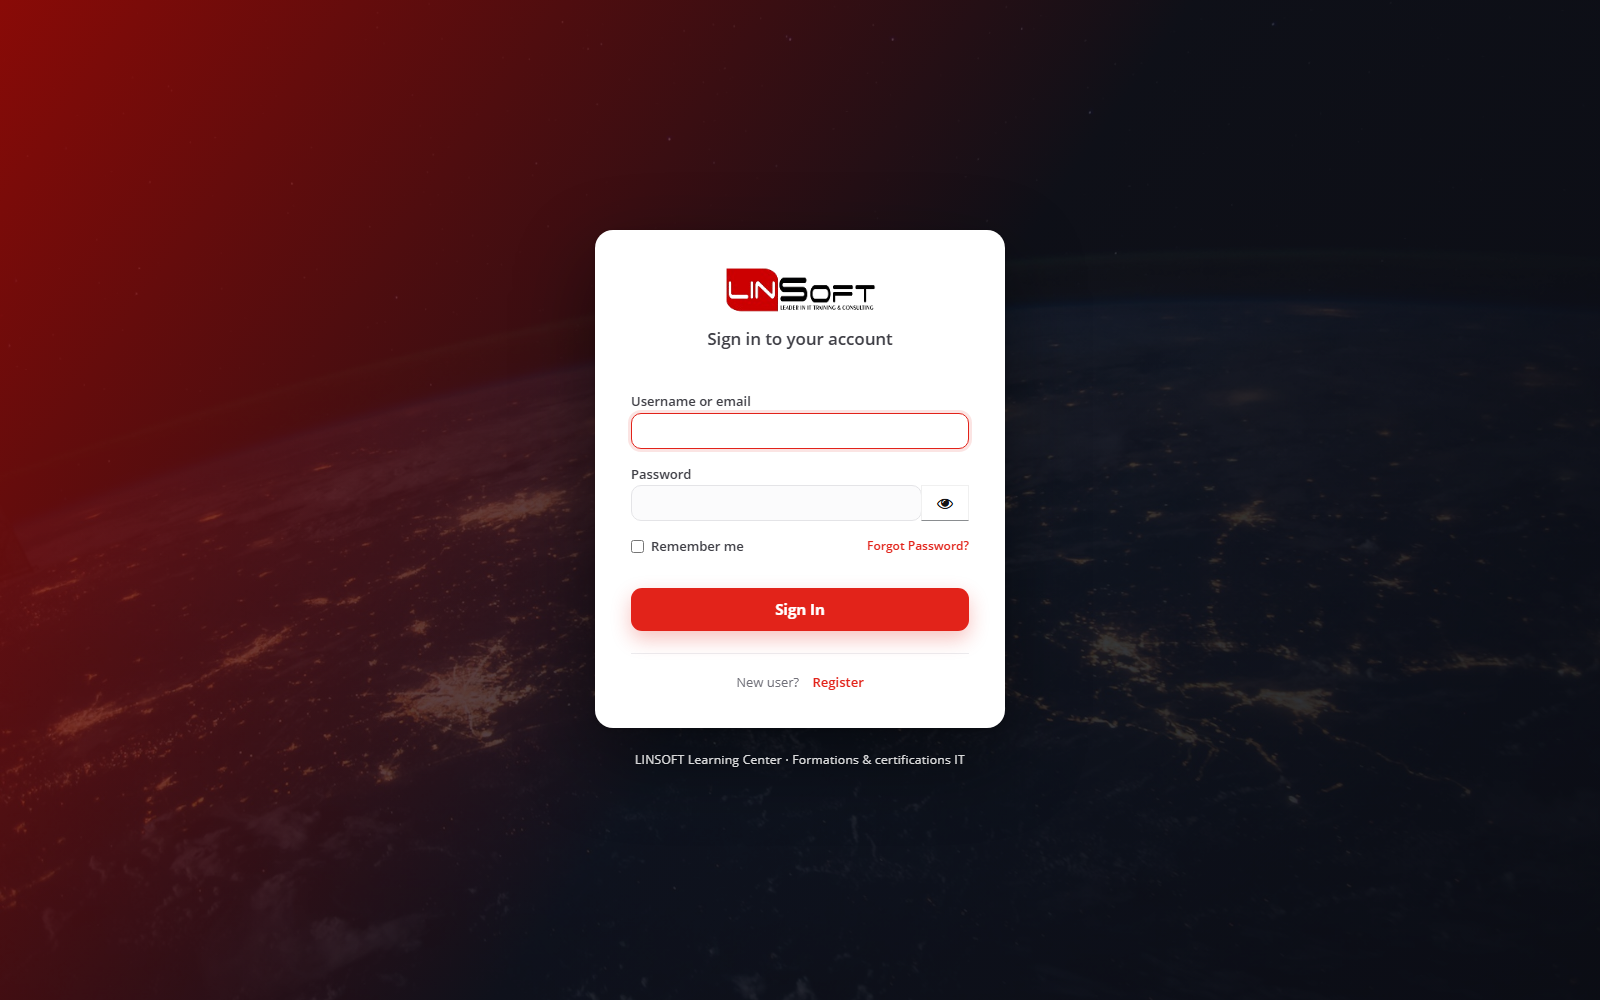
\includegraphics[width=0.92\textwidth]{captures/02-connexion-keycloak.png}
  \caption{Authentification déléguée à Keycloak, traversée automatiquement par les tests}
  \label{fig:e2e-login}
\end{figure}

Les scénarios couvrent l'authentification de chaque rôle, le rejet d'identifiants
invalides, et surtout le \textbf{cloisonnement} : un participant qui saisit l'adresse de
la console d'administration est détourné, un formateur ne peut pas atteindre la gestion des
certificats.

\begin{figure}[H]\centering
  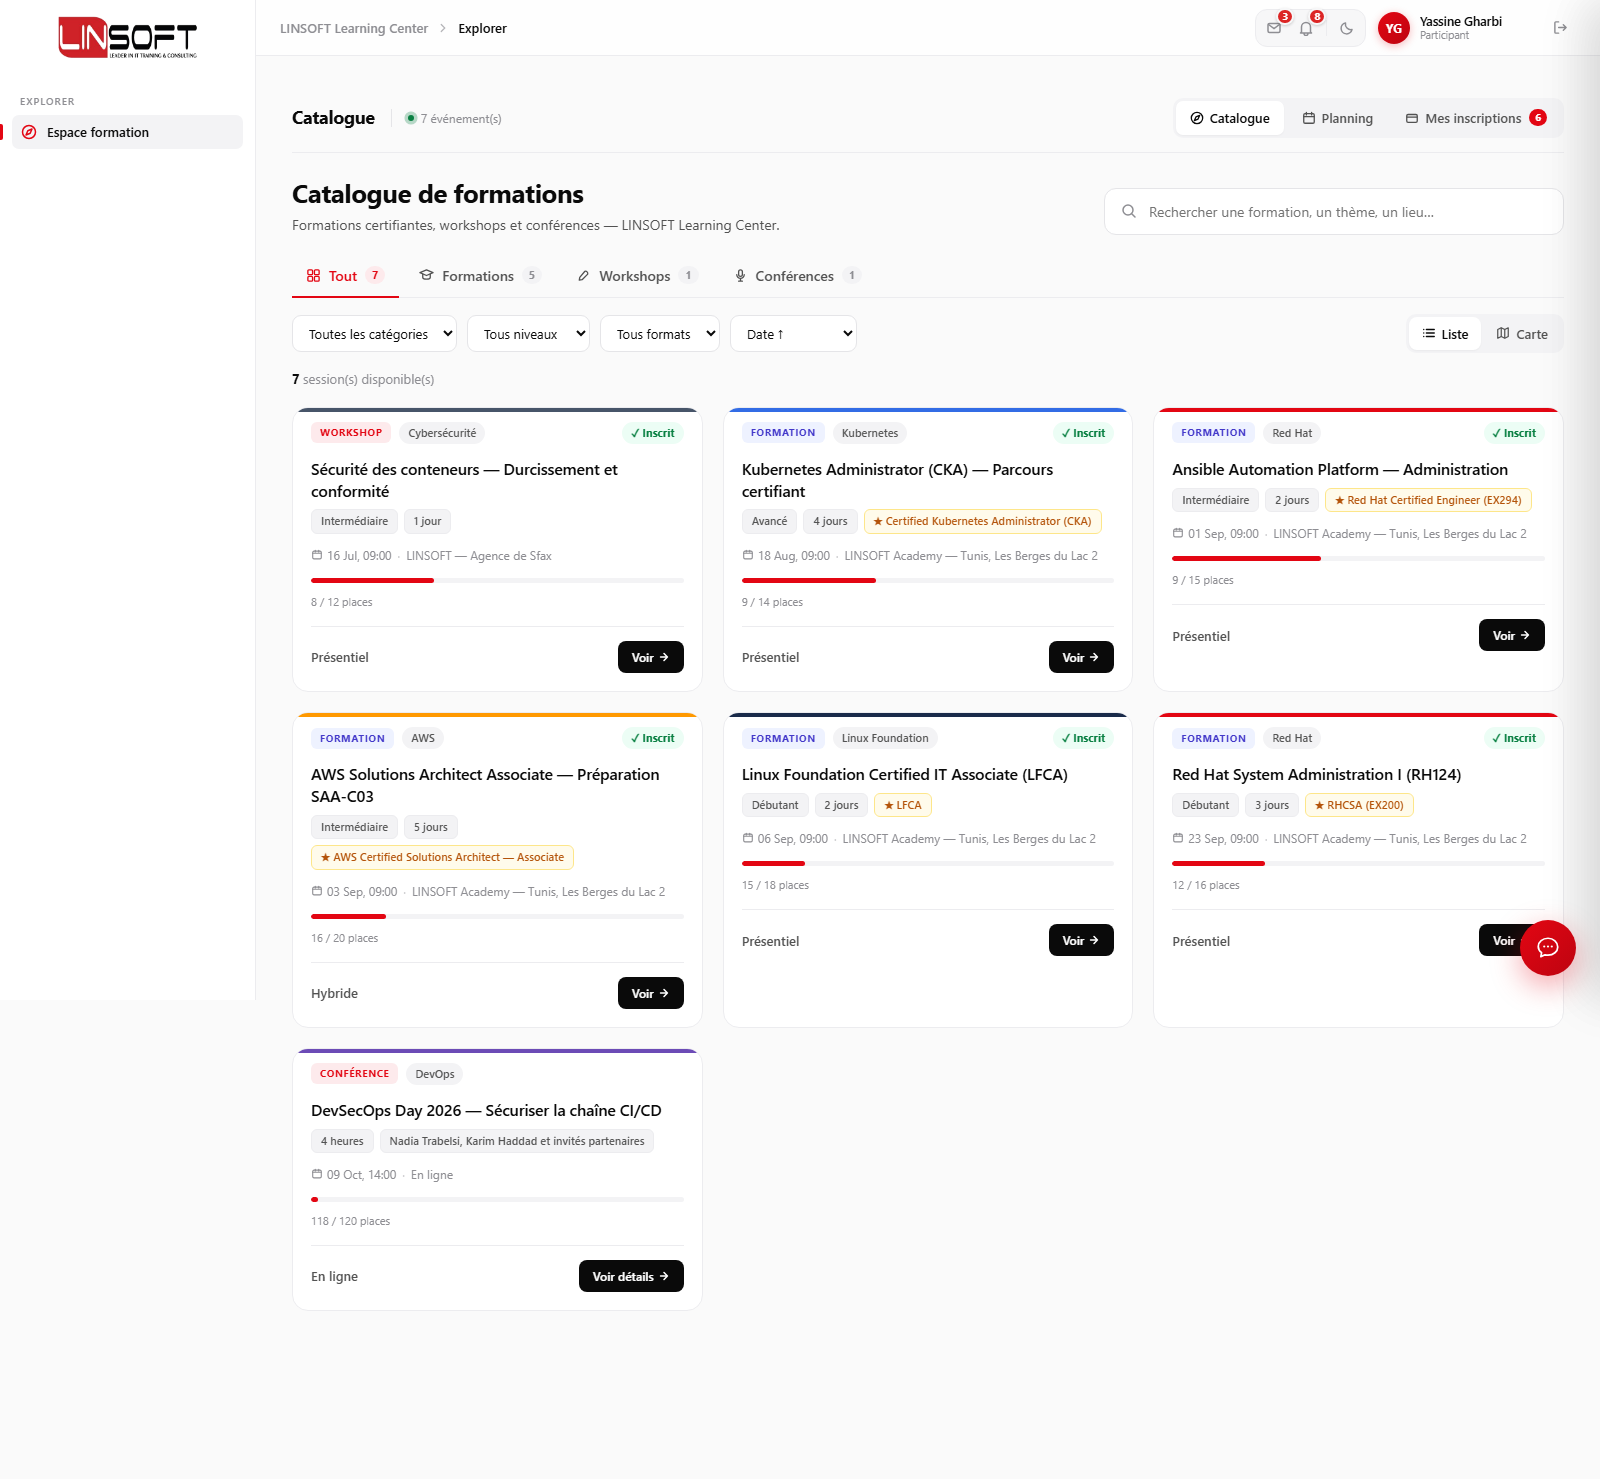
\includegraphics[width=0.92\textwidth]{captures/03-catalogue.png}
  \caption{Catalogue de formations — vue participant}
  \label{fig:devops-catalogue}
\end{figure}

%============================================================================
\section{Qualité du code et couverture}

\subsection{Outils d'analyse}
L'analyse statique (\textbf{Checkstyle} et \textbf{SpotBugs}) est regroupée dans un profil
Maven \texttt{quality}, activé à la demande et en intégration continue. Le jeu de règles
Checkstyle cible délibérément les défauts réels — comparaison de chaînes par
\texttt{==}, \texttt{equals} sans \texttt{hashCode}, blocs \texttt{catch} vides,
\texttt{switch} sans \texttt{default} — plutôt que la mise en forme : un jeu de règles trop
bavard finit systématiquement désactivé.

\subsection{Couverture mesurée}
\textbf{JaCoCo} produit des rapports HTML et XML par module. Le seuil est vérifié à chaque
\texttt{mvn verify} et fait échouer le build s'il n'est pas atteint.

\begin{table}[H]\centering\renewcommand{\arraystretch}{1.25}
\begin{tabular}{|p{5.5cm}|p{3cm}|}\hline
\rowcolor{gray!15}\textbf{Module} & \textbf{Couverture} \\ \hline
\texttt{feedback-service} & 78~\% \\ \hline
\texttt{notification-service} & 74~\% \\ \hline
\texttt{ticket-service} & 71~\% \\ \hline
\texttt{registration-service} & 61~\% \\ \hline
\texttt{event-service} & 53~\% \\ \hline
\texttt{ai-service} & 42~\% \\ \hline
\texttt{user-service} & 41~\% \\ \hline
\end{tabular}
\caption{Couverture des instructions, hors configuration, entités et DTO}\label{tab:couverture}
\end{table}

Le seuil a été relevé progressivement (0~\%, puis 25~\%, 30~\% et enfin 40~\%) au fur et à
mesure de l'écriture des tests. Ce choix est délibéré : un seuil ambitieux fixé d'emblée
aurait été inatteignable et n'aurait produit qu'une chose, sa propre désactivation. Le
seuil joue ainsi le rôle d'un \emph{cliquet anti-régression} plutôt que d'un objectif
décoratif. Son caractère réellement bloquant a été vérifié en le forçant temporairement à
90~\%, ce qui provoque bien l'échec du build.

%============================================================================
\section{Conteneurisation}

Chacun des onze composants dispose de son image. Les images backend reposent sur
\texttt{eclipse-temurin:17-jre-alpine} et appliquent \texttt{chgrp -R 0 /app}, condition
nécessaire sur OpenShift, qui exécute les conteneurs avec un identifiant utilisateur
aléatoire appartenant au groupe~0. Le frontend est construit en deux étapes
(\texttt{node:20-alpine} puis \texttt{nginx-unprivileged}) et s'exécute sans privilèges.

\subsection{Un défaut de conception corrigé}
Les images déclaraient déjà une directive \texttt{HEALTHCHECK} interrogeant
\texttt{/actuator/health}, \textbf{mais sept services sur dix n'embarquaient pas Actuator} :
la sonde recevait une réponse 404. Le fichier \texttt{docker-compose.yml} contournait le
problème par un \texttt{curl -s -o /dev/null || exit 1}, qui \emph{réussit même sur un 404
ou un 401}. Aucune vérification de santé du projet ne prouvait donc quoi que ce soit.
Actuator a été ajouté à tous les services via le POM parent, et les contournements
remplacés par de véritables vérifications.

%============================================================================
\section{Intégration et livraison continues}

\subsection{Architecture du pipeline}
La chaîne est décrite dans \texttt{.github/workflows/ci.yml} et s'exécute sur
\textbf{GitHub Actions} à chaque poussée et à chaque \emph{pull request}.

\begin{table}[H]\centering\renewcommand{\arraystretch}{1.25}
\begin{tabular}{|p{4cm}|p{9.5cm}|}\hline
\rowcolor{gray!15}\textbf{Étape} & \textbf{Contenu} \\ \hline
Tests backend & \texttt{mvn verify} : unitaires, API/sécurité, intégration, couverture \\ \hline
Analyse statique & Checkstyle et SpotBugs \\ \hline
Tests frontend & Vitest puis build de production \\ \hline
Images Docker & Onze images construites en parallèle \\ \hline
Analyse de sécurité & Trivy, vulnérabilités critiques et élevées \\ \hline
Publication & Registre GHCR, branche principale uniquement \\ \hline
Tests E2E & Plateforme complète démarrée, jeu de données semé, Playwright \\ \hline
\end{tabular}
\caption{Étapes de la chaîne d'intégration continue}\label{tab:pipeline}
\end{table}

\subsection{Choix : ne pas compiler dans les images}
Les fichiers \texttt{Dockerfile} du backend copient une archive JAR déjà construite plutôt
que de la compiler. Une construction multi-étapes par service recompilerait dix fois le même
réacteur Maven, pour un résultat identique. Le réacteur est donc construit \textbf{une
seule fois}, les archives circulent en artefact entre les étapes, et chaque image est
assemblée à partir du binaire validé : l'artefact testé et l'artefact publié sont ainsi le
même objet.

\subsection{Garde-fou contre les faux positifs}
Une étape vérifie explicitement qu'\textbf{aucun test d'intégration n'a été ignoré} alors
que Docker était disponible. Sans ce contrôle, un environnement dépourvu de Docker
produirait un pipeline vert trompeur, puisque les tests Testcontainers s'ignorent
automatiquement en l'absence de démon.

\subsection{Deux défauts révélés par les premières exécutions}
Aucun des deux n'était détectable en local, ce qui illustre précisément l'apport d'une
chaîne d'intégration continue.

\begin{enumerate}
  \item \textbf{Référence d'action non résolue.} Les onze tâches de construction d'images
        échouaient à l'étape « Set up job », c'est-à-dire \emph{avant} leur première
        instruction. Les étiquettes du dépôt \texttt{trivy-action} sont préfixées par
        \texttt{v} : la référence \texttt{@0.28.0} n'existait pas. GitHub Actions résout les
        actions avant de les exécuter, d'où un échec sans aucune trace dans les étapes.
  \item \textbf{Nom d'image refusé par le registre.} Une fois ce point corrigé, la
        construction, l'analyse Trivy et l'authentification réussissaient, mais la
        publication échouait — symptôme trompeur. Le compte GitHub s'écrit
        \texttt{Medamine009}, avec une majuscule, alors que GHCR n'accepte que des noms
        d'image en minuscules. Le nom est désormais normalisé avant usage.
\end{enumerate}

%============================================================================
\section{Supervision et observabilité}

\subsection{Points de mesure}
Tous les services exposent, via Actuator et Micrometer, un agrégat de santé, des sondes
distinctes de \emph{liveness} et de \emph{readiness}, ainsi que leurs métriques au format
Prometheus. L'exposition est volontairement restreinte aux points réellement utilisés :
\texttt{env}, \texttt{beans} et \texttt{heapdump} restent fermés.

\subsection{Collecte et visualisation}
Prometheus interroge les dix services toutes les quinze secondes ; Grafana en propose la
lecture. L'ensemble est placé derrière un profil Docker Compose afin de ne pas alourdir le
démarrage courant de la plateforme.

\begin{figure}[H]\centering
  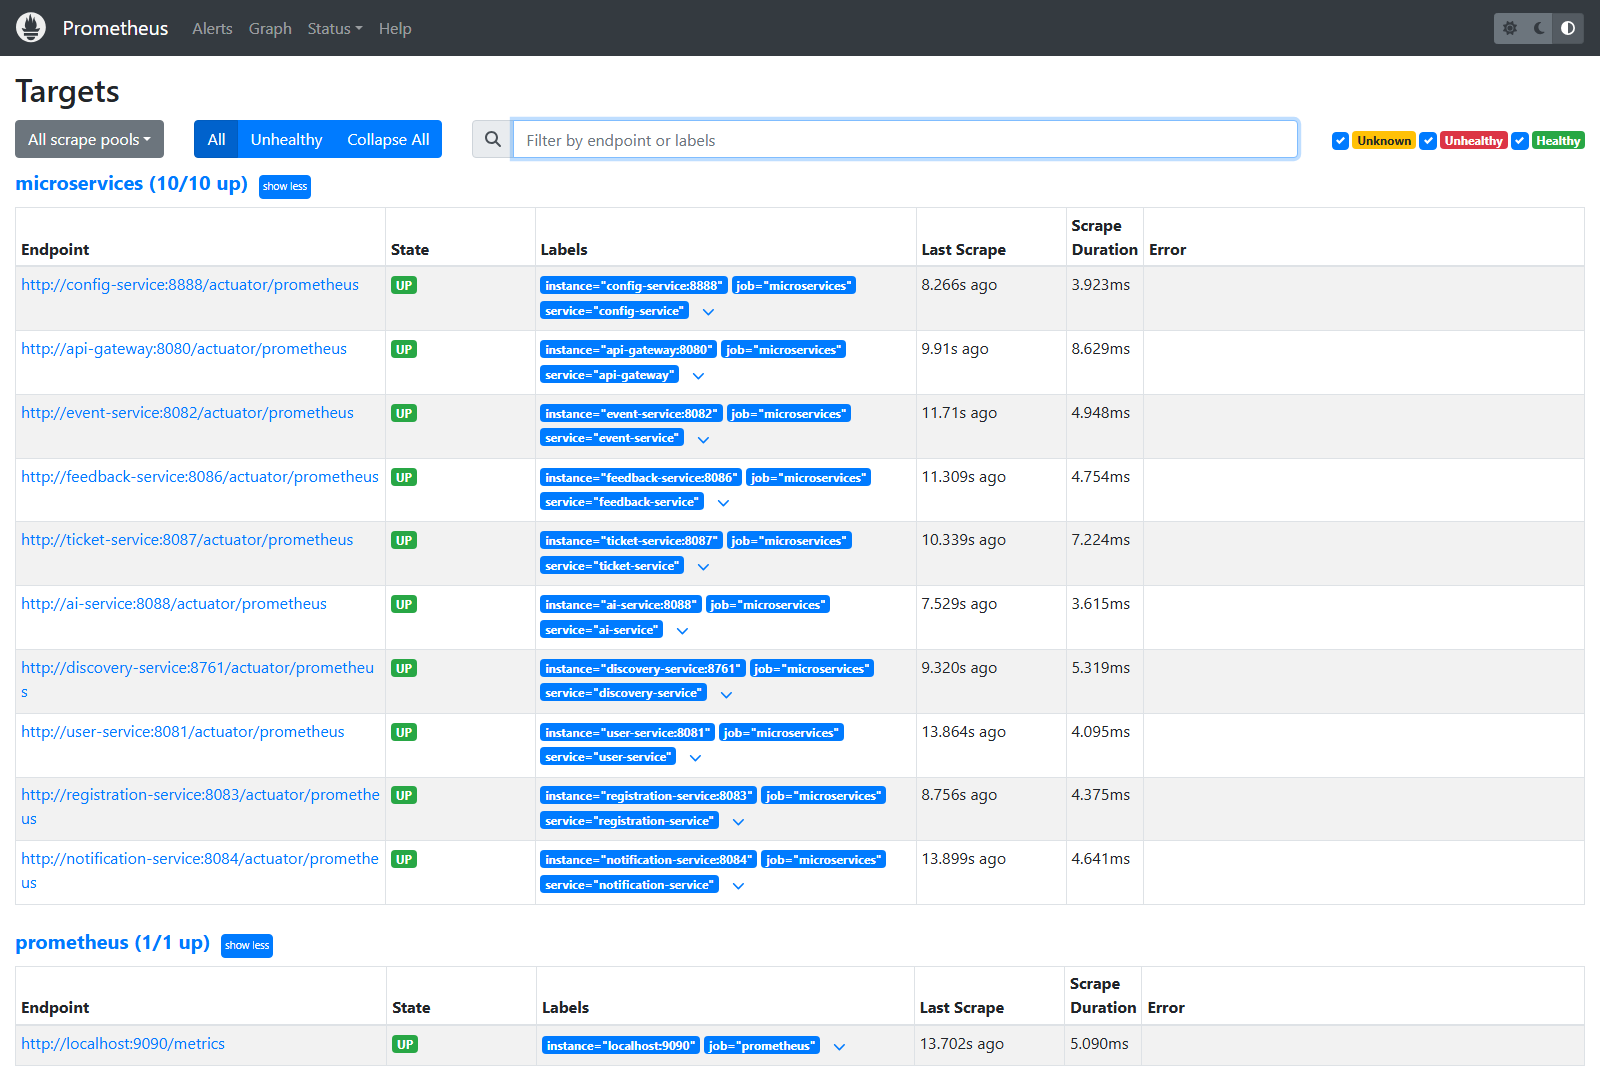
\includegraphics[width=0.92\textwidth]{captures/08-prometheus-cibles.png}
  \caption{Cibles Prometheus : les dix microservices interrogés avec succès}
  \label{fig:prometheus}
\end{figure}

\begin{figure}[H]\centering
  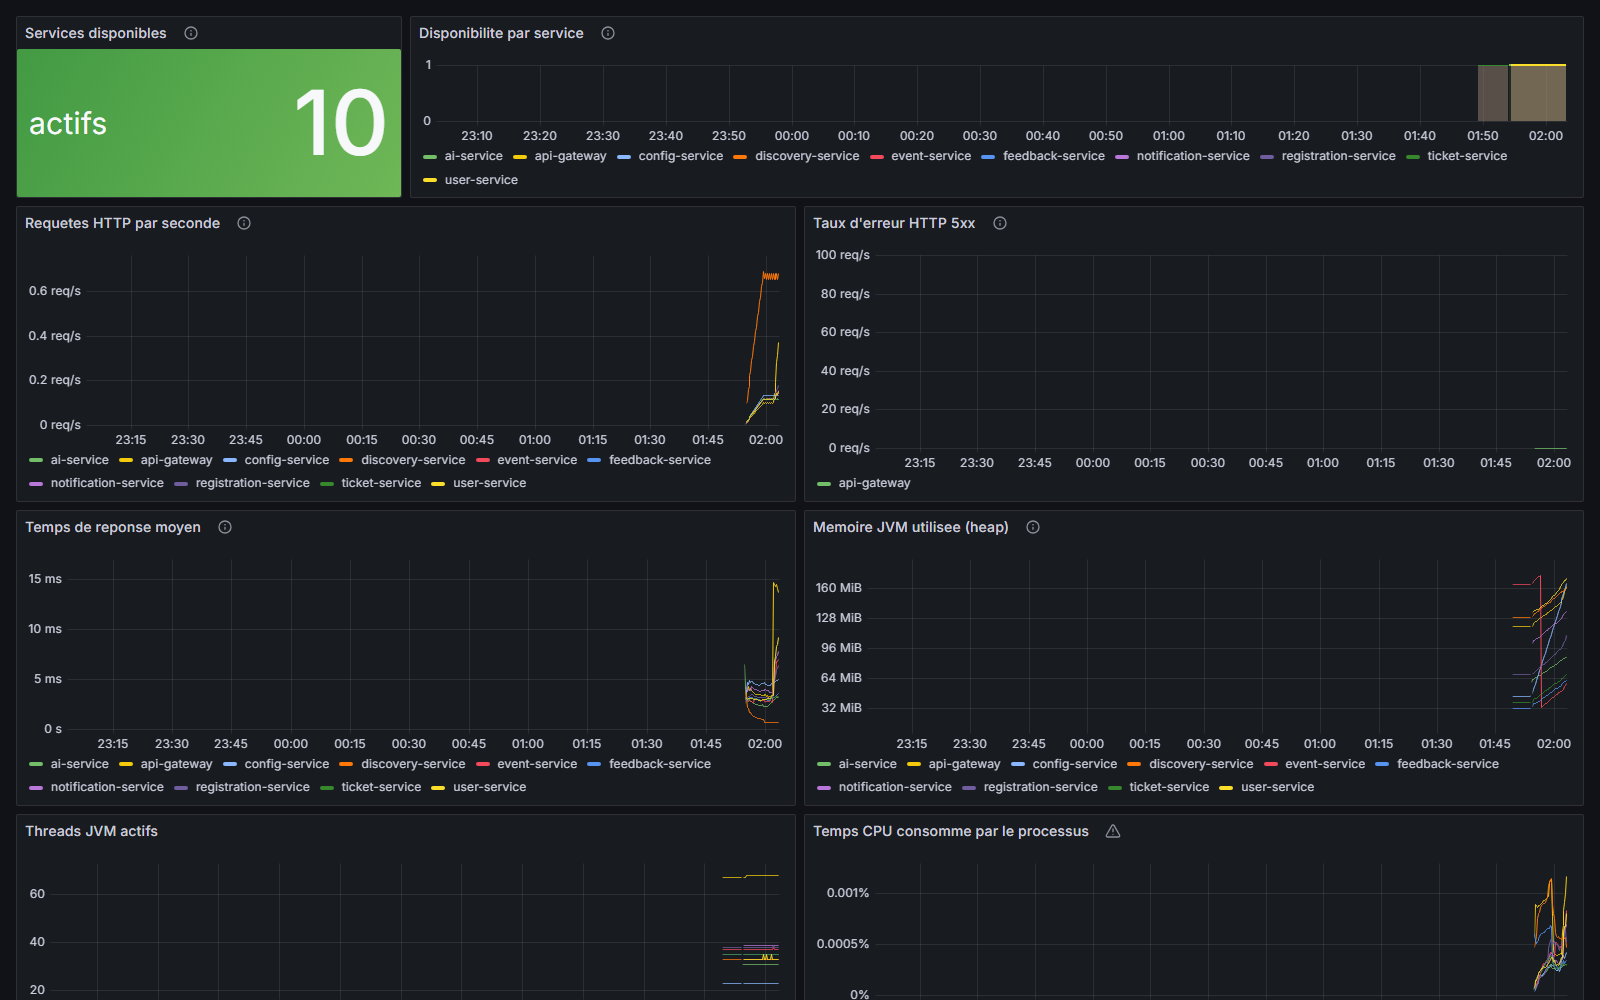
\includegraphics[width=\textwidth]{captures/09-grafana-plateforme.png}
  \caption{Tableau de bord Grafana : disponibilité, charge, temps de réponse et mémoire}
  \label{fig:grafana}
\end{figure}

Chaque série porte une étiquette \texttt{application} apposée par Micrometer ; sans elle,
les séries des dix services seraient indistinguables.

\begin{figure}[H]\centering
  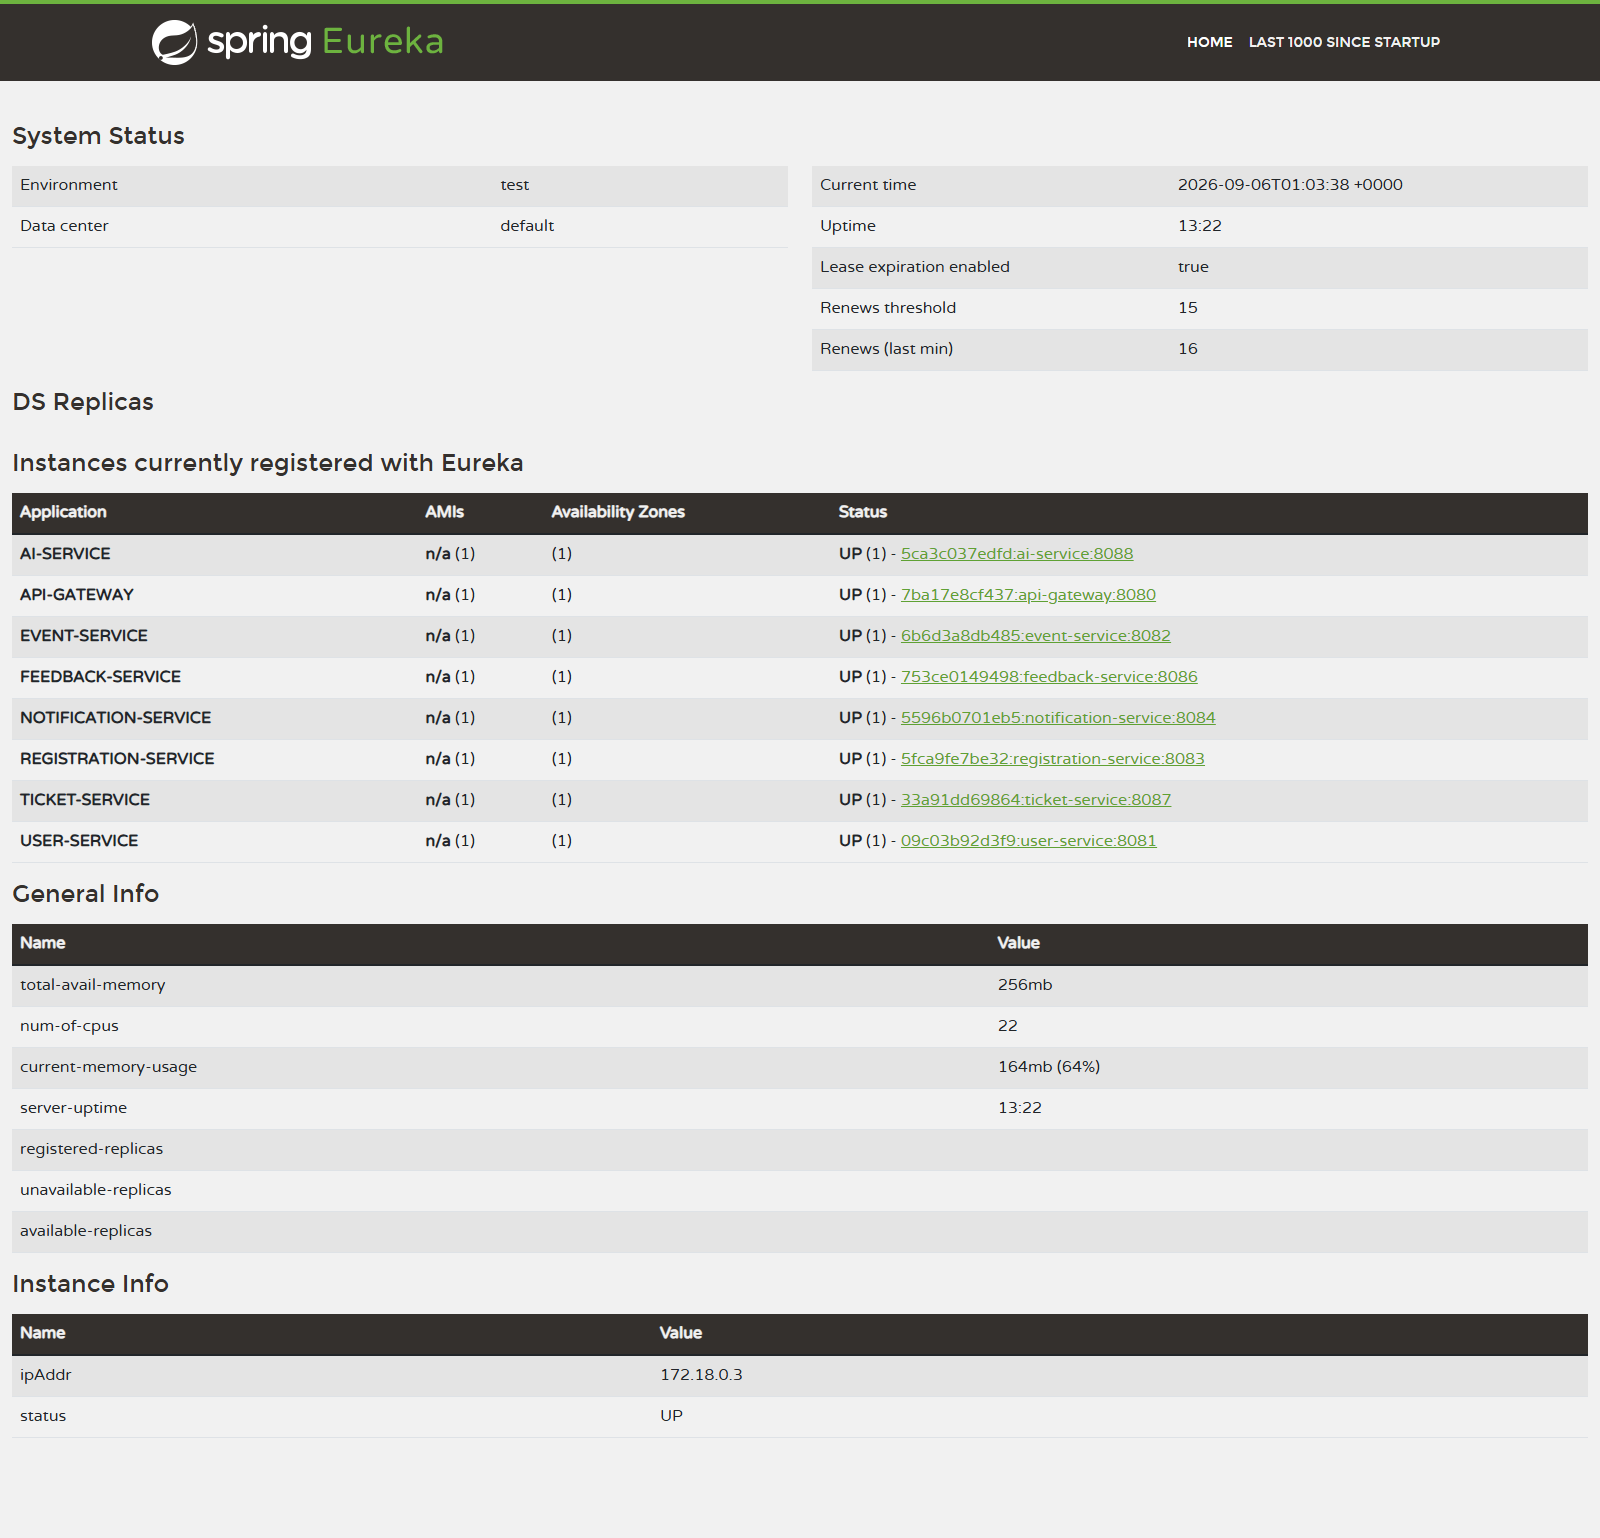
\includegraphics[width=0.92\textwidth]{captures/11-eureka.png}
  \caption{Registre Eureka : services enregistrés et découverte dynamique}
  \label{fig:eureka}
\end{figure}

\begin{figure}[H]\centering
  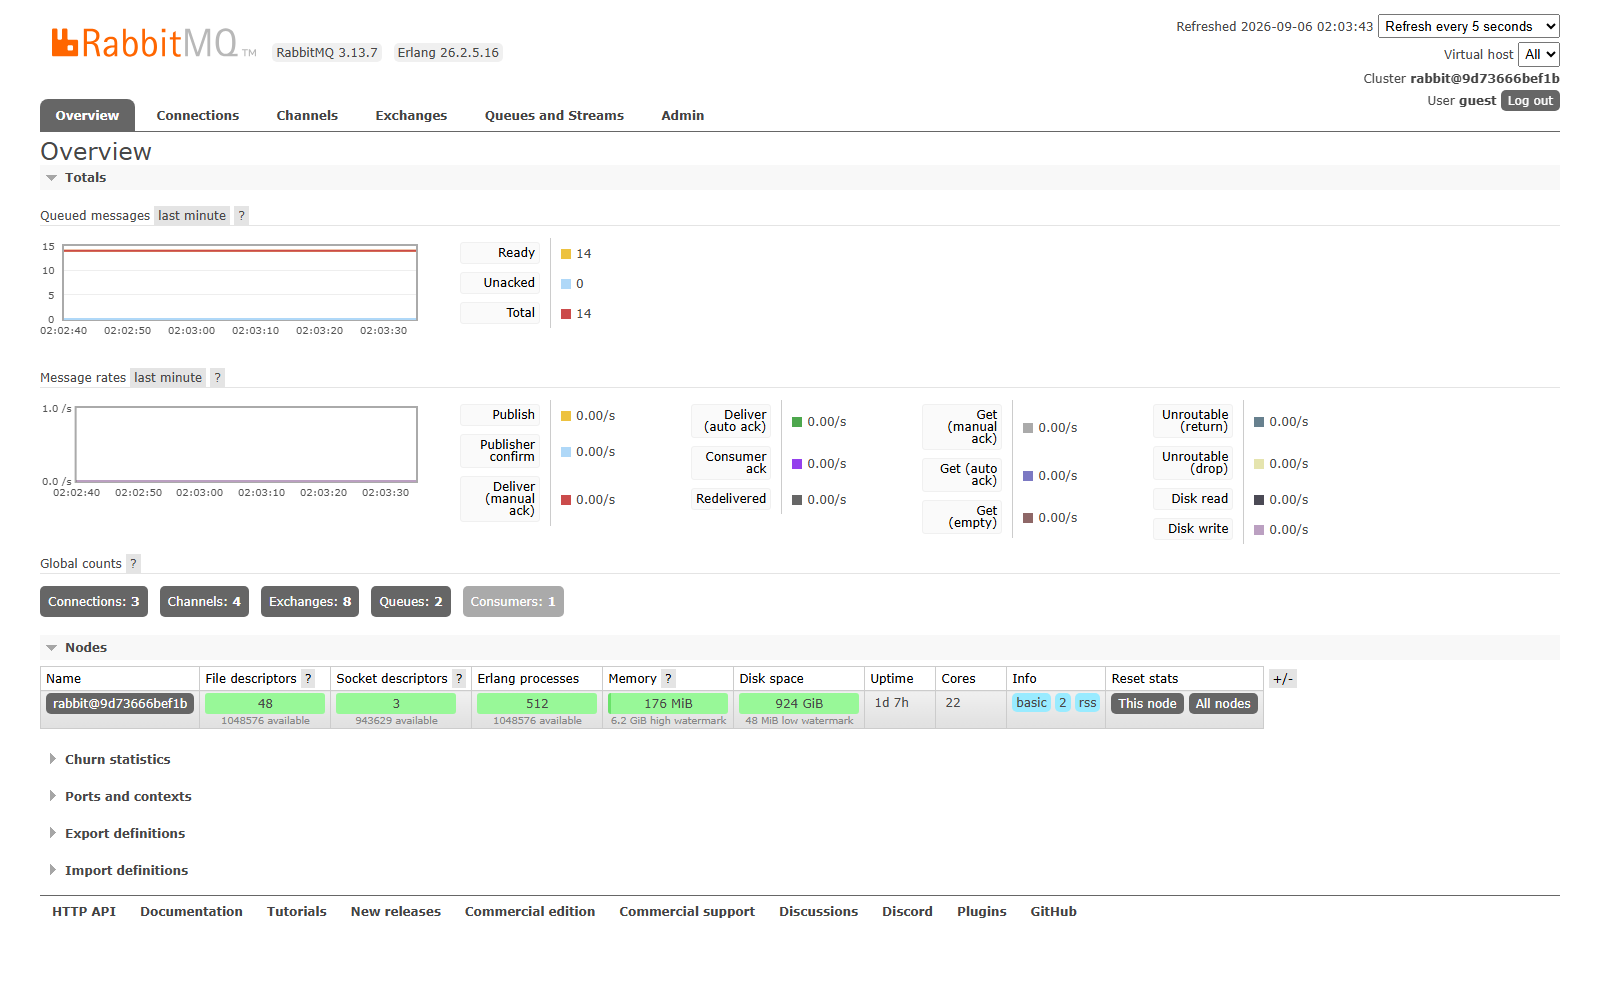
\includegraphics[width=0.92\textwidth]{captures/12-rabbitmq.png}
  \caption{Console RabbitMQ : file de notifications et débit des messages}
  \label{fig:rabbitmq}
\end{figure}

%============================================================================
\section{Sécurité de la chaîne}

\begin{itemize}
  \item \textbf{Analyse des images} : Trivy inspecte chaque image et remonte les
        vulnérabilités critiques et élevées dans l'onglet \emph{Security} du dépôt.
  \item \textbf{Aucun secret versionné} : la publication utilise le jeton fourni par la
        plateforme. Le fichier \texttt{.env} est exclu du dépôt et accompagné d'un modèle
        \texttt{.env.example}.
  \item \textbf{Secrets de déploiement} : un script \texttt{create-secrets.sh} génère des
        mots de passe aléatoires via \texttt{oc create secret}, de sorte qu'aucune valeur
        réelle ne transite par Git.
\end{itemize}

%============================================================================
\section{Illustrations du parcours fonctionnel}

Les captures suivantes montrent le résultat obtenu sur les fonctionnalités les plus
structurantes, avec le jeu de données de démonstration.

\begin{figure}[H]\centering
  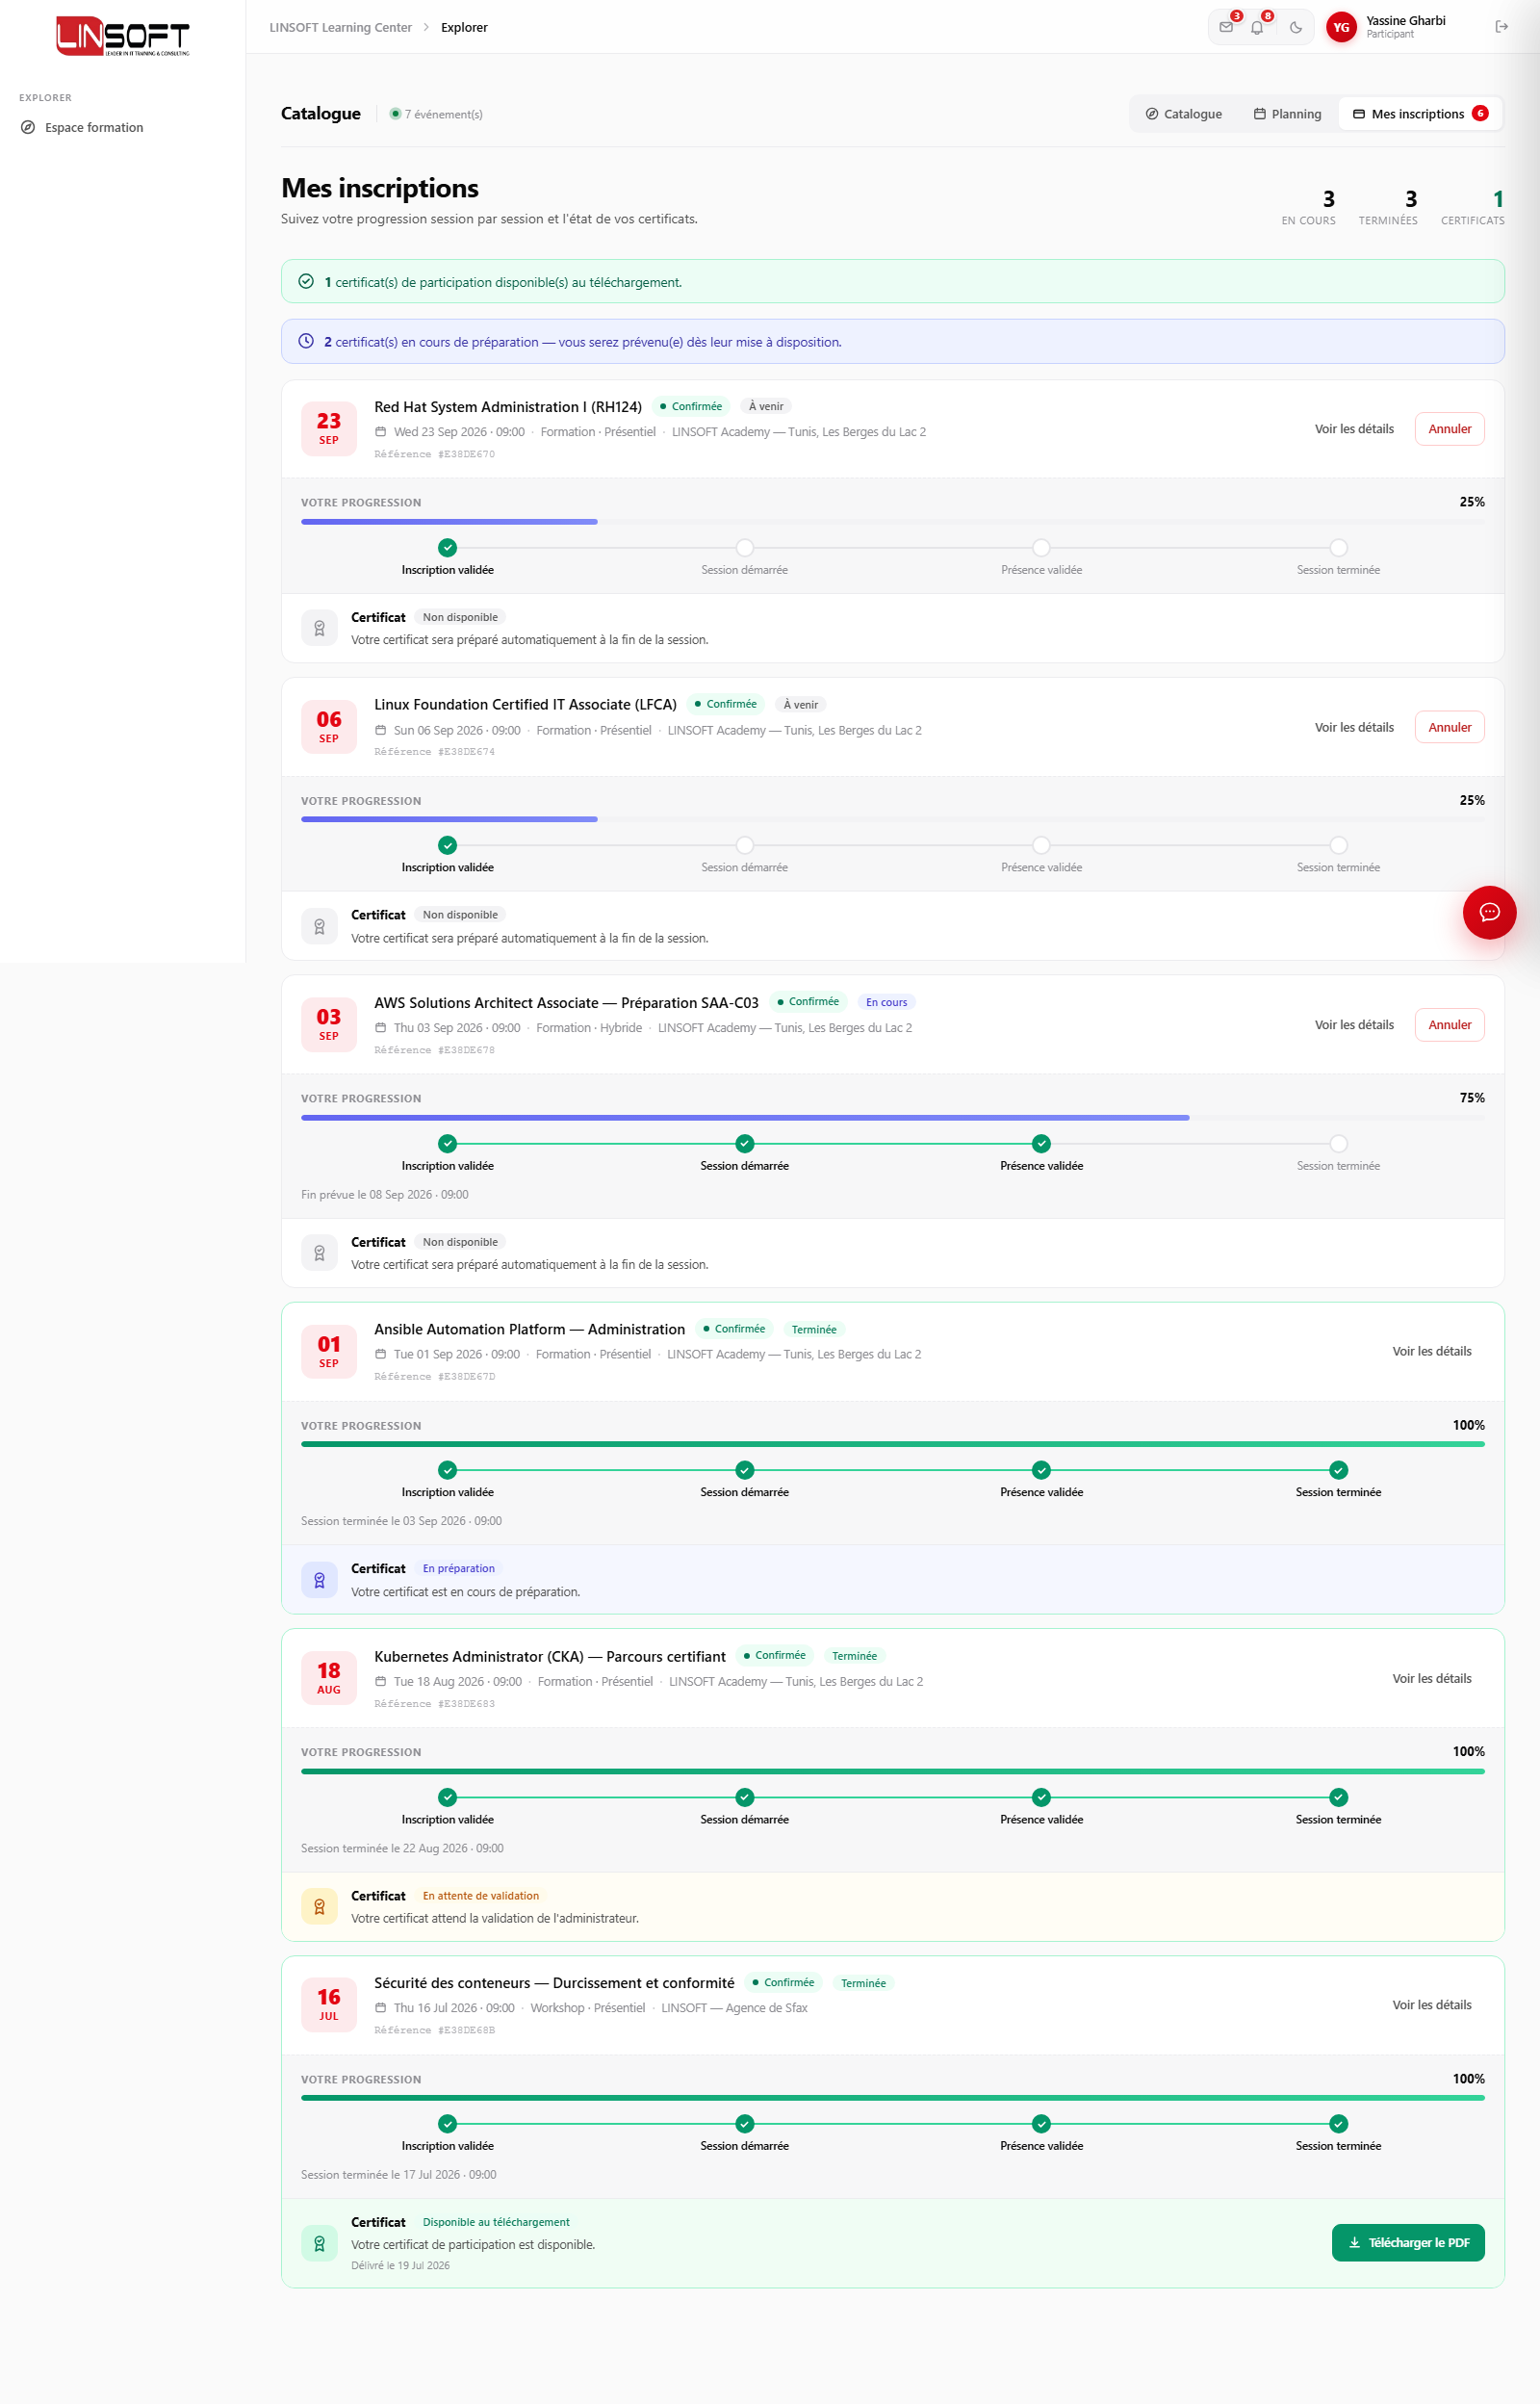
\includegraphics[width=0.85\textwidth]{captures/04-suivi-certificats.png}
  \caption{Suivi de participation : progression par jalons et cycle de vie du certificat}
  \label{fig:suivi}
\end{figure}

Cette vue rassemble les cinq états du parcours : session à venir (certificat non
disponible), session en cours avec progression intermédiaire, puis session terminée avec un
certificat successivement \emph{en préparation}, \emph{en attente de validation} et enfin
\emph{disponible au téléchargement}.

\begin{figure}[H]\centering
  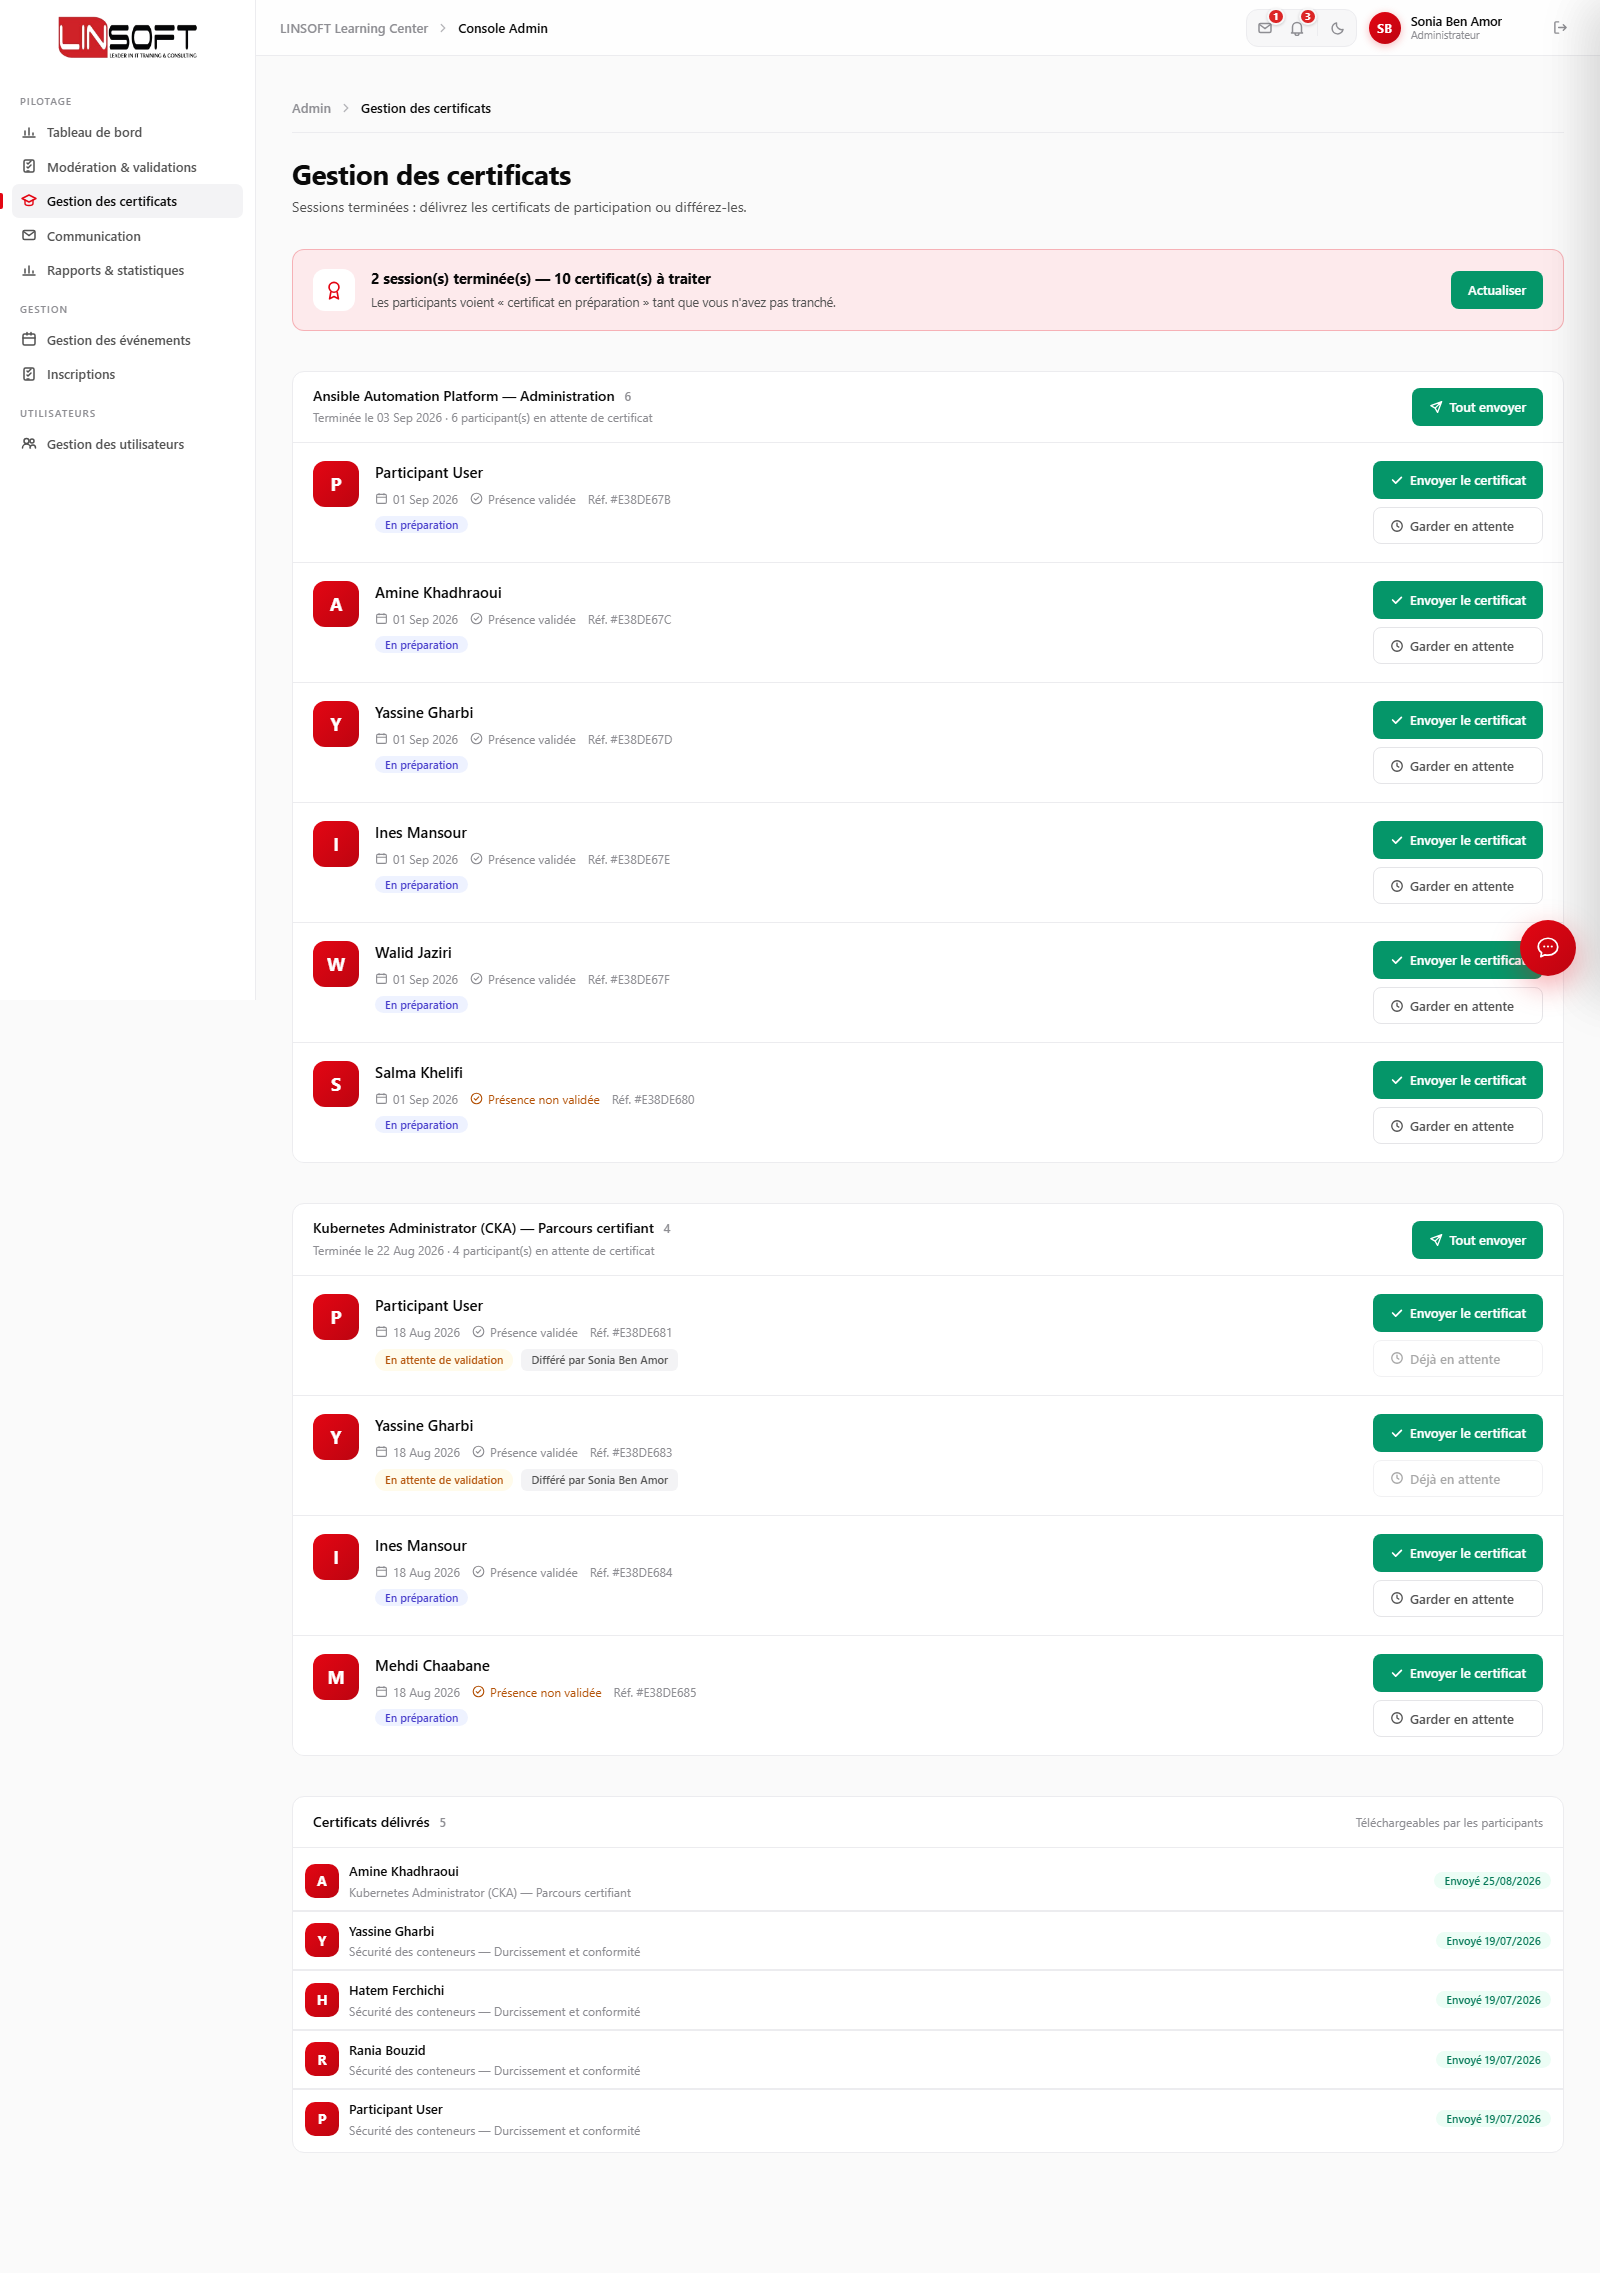
\includegraphics[width=0.85\textwidth]{captures/06-gestion-certificats.png}
  \caption{Console d'administration : file des certificats à délivrer, groupée par session}
  \label{fig:certificats-admin}
\end{figure}

\begin{figure}[H]\centering
  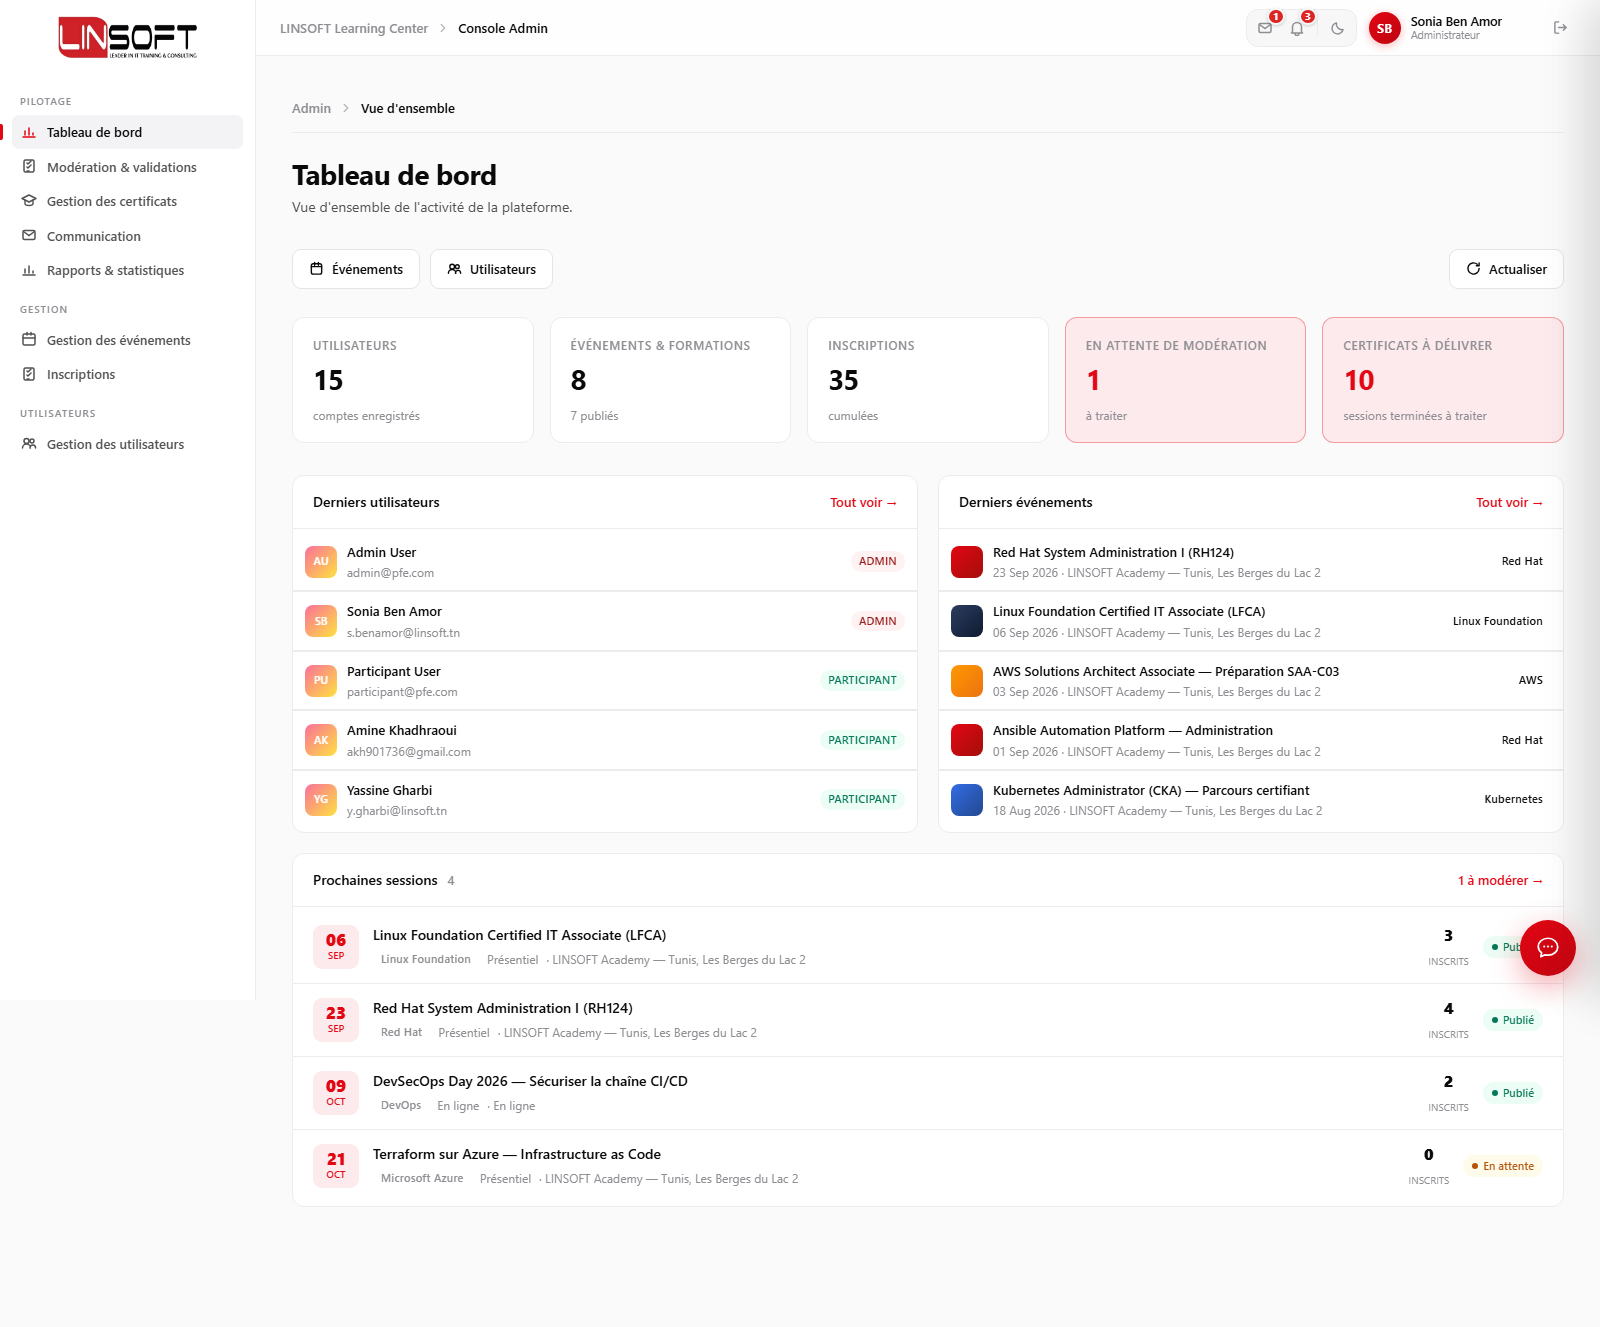
\includegraphics[width=0.92\textwidth]{captures/05-admin-dashboard.png}
  \caption{Tableau de bord administrateur et indicateurs de la plateforme}
  \label{fig:admin}
\end{figure}

\begin{figure}[H]\centering
  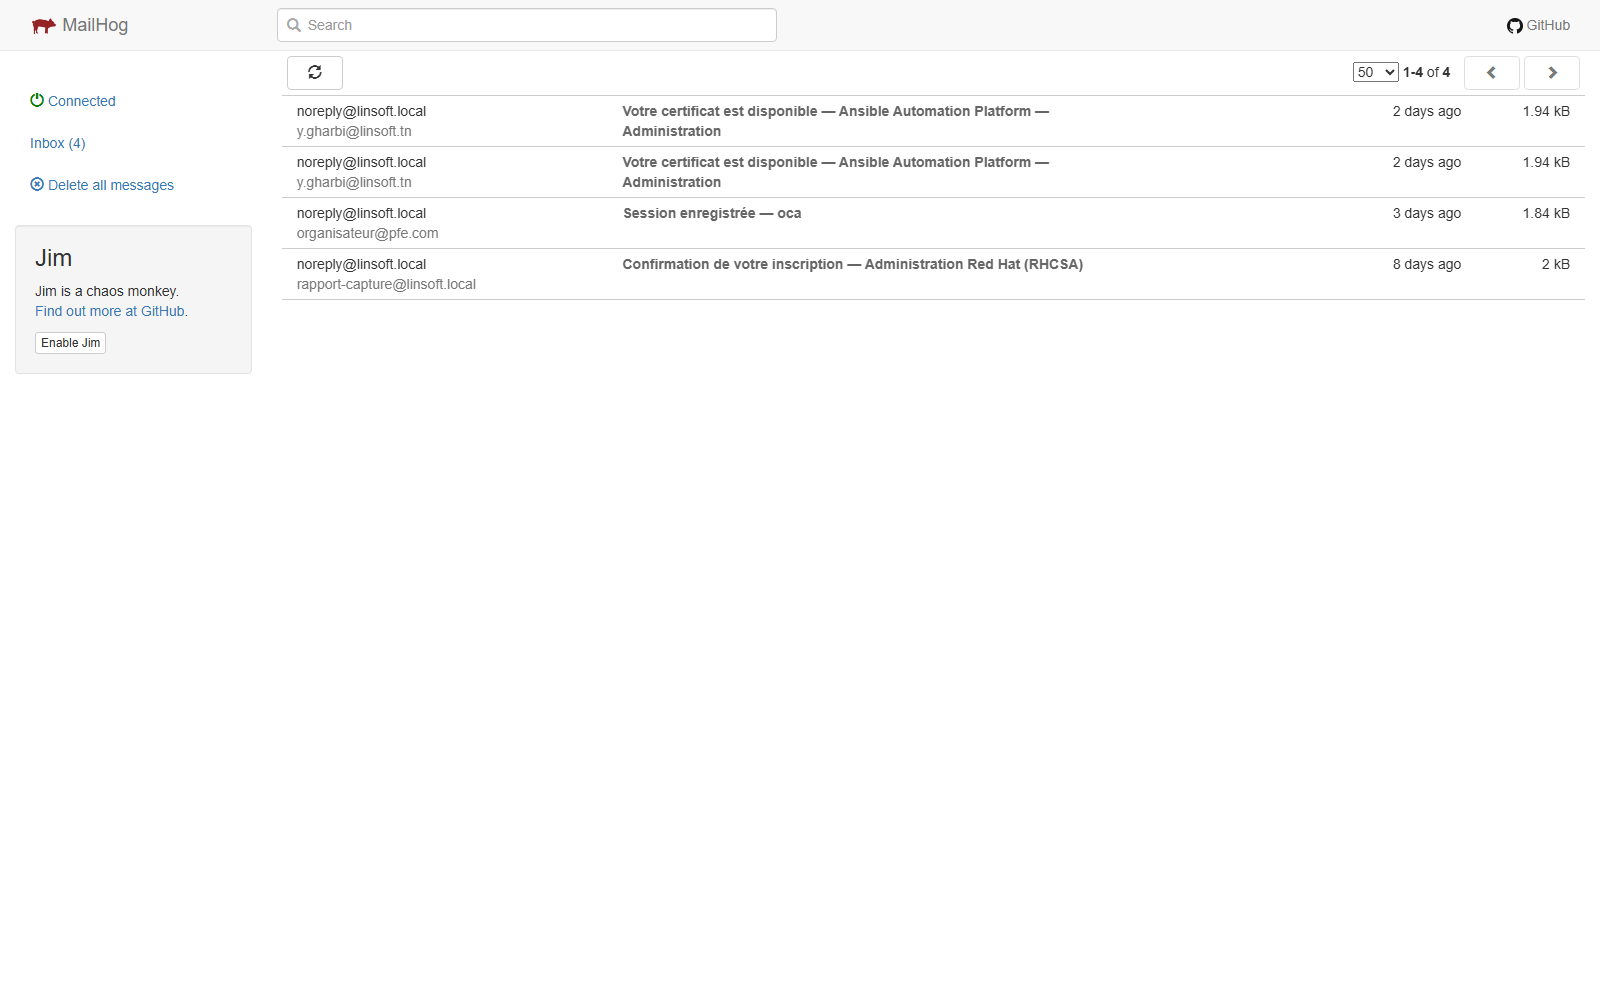
\includegraphics[width=0.92\textwidth]{captures/10-mailhog.png}
  \caption{Courriels émis par la plateforme, interceptés par MailHog en environnement de test}
  \label{fig:mailhog}
\end{figure}

%============================================================================
\section*{Conclusion}
La démarche présentée dans ce chapitre a fait passer le projet de dix-huit tests sans mesure
de couverture à près de trois cents tests répartis sur quatre niveaux, adossés à une chaîne
d'intégration continue de dix-sept tâches et à un dispositif de supervision opérationnel.
Au-delà des chiffres, cette démarche a démontré sa valeur en révélant des défauts réels et
invisibles autrement : des vérifications de santé qui ne vérifiaient rien, une référence
d'action inexistante, un nom d'image refusé par le registre, et une référence de dossier
identique pour toute une promotion de participants.

%  Les captures référencées se trouvent dans rapport-pfe/captures/
%############################################################################
\chapter{Tests, qualité et démarche DevOps}

\section*{Introduction}
Une plateforme composée de dix microservices ne se valide pas en la parcourant à la main :
le nombre de combinaisons de rôles, d'états et de services rend la vérification manuelle
à la fois incomplète et non reproductible. Ce chapitre présente la stratégie de test mise
en place, les outils de mesure de la qualité, la chaîne d'intégration continue et le
dispositif de supervision. Chaque choix y est justifié par le défaut qu'il permet de
détecter, et les résultats présentés sont ceux réellement obtenus sur la plateforme.

%============================================================================
\section{Stratégie de test}

\subsection{Pyramide de test retenue}
Quatre niveaux de test se répondent, chacun apportant une garantie que les autres ne
peuvent pas fournir.

\begin{table}[H]\centering\renewcommand{\arraystretch}{1.3}
\begin{tabular}{|p{3.2cm}|p{5cm}|p{6cm}|}\hline
\rowcolor{gray!15}\textbf{Niveau} & \textbf{Outils} & \textbf{Question à laquelle il répond} \\ \hline
Unitaire & JUnit 5, Mockito & La règle métier est-elle juste ? \\ \hline
API / Sécurité & MockMvc, spring-security-test & L'API applique-t-elle réellement les droits ? \\ \hline
Intégration & Testcontainers (MongoDB) & Le code dialogue-t-il correctement avec une base réelle ? \\ \hline
Bout en bout & Playwright, Chromium & Le parcours utilisateur fonctionne-t-il entièrement ? \\ \hline
\end{tabular}
\caption{Niveaux de test et rôle de chacun}\label{tab:pyramide}
\end{table}

\subsection{Séparation des tests rapides et des tests d'infrastructure}
La convention de nommage pilote l'exécution, configurée une seule fois dans le POM parent :
les classes \texttt{*Test} sont exécutées par Surefire pendant la phase \texttt{test}, les
classes \texttt{*IT} par Failsafe pendant la phase \texttt{verify}. Le développeur dispose
ainsi d'une boucle de retour courte (\texttt{mvn test}, sans infrastructure), tandis que
l'intégration continue exécute la chaîne complète (\texttt{mvn verify}).

\subsection{Répartition obtenue}
\begin{table}[H]\centering\renewcommand{\arraystretch}{1.25}
\begin{tabular}{|p{5cm}|p{2.6cm}|p{2.6cm}|}\hline
\rowcolor{gray!15}\textbf{Périmètre} & \textbf{Avant} & \textbf{Après} \\ \hline
Tests backend & 18 & \textbf{195} \\ \hline
Tests frontend & 53 (dont 1 en échec) & \textbf{82} \\ \hline
Tests de bout en bout & 0 & \textbf{14} \\ \hline
Mesure de couverture & aucune & JaCoCo, seuil à 40~\% \\ \hline
\end{tabular}
\caption{Évolution de la couverture de test du projet}\label{tab:devops-tests}
\end{table}

\subsection{Exemples de règles protégées}
Les tests ne visent pas le taux de couverture pour lui-même, mais les règles dont la
défaillance produirait un défaut visible :

\begin{itemize}
  \item l'annulation d'une \emph{demande en attente} ne doit pas libérer une place qui
        n'avait jamais été réservée, sous peine de créer des places fantômes ;
  \item un second scan du même QR code renvoie \texttt{ALREADY} plutôt que d'autoriser
        une seconde entrée ;
  \item l'envoi d'un certificat est idempotent : un double clic de l'administrateur ne
        déclenche pas un second courriel ;
  \item un message RabbitMQ malformé ne doit pas remonter en exception, sans quoi le
        courtier le redistribuerait en boucle et bloquerait la file pour tous les
        destinataires ;
  \item une session dont la durée est illisible n'est jamais clôturée par anticipation :
        le calcul retombe sur une journée type.
\end{itemize}

\subsection{Tests de sécurité}
Les tests de contrôleur chargent la \textbf{configuration de sécurité de production}
(\texttt{@Import(SecurityConfig.class)}) et non une sécurité désactivée : ce qui est
vérifié est donc bien ce qui s'appliquera en exploitation. Des jetons JWT sont simulés
avec les rôles Keycloak correspondants.

\begin{table}[H]\centering\renewcommand{\arraystretch}{1.25}
\begin{tabular}{|p{8.5cm}|p{4cm}|}\hline
\rowcolor{gray!15}\textbf{Scénario} & \textbf{Réponse attendue} \\ \hline
Appel sans jeton & \texttt{401} \\ \hline
Vérification publique d'un billet & \texttt{200} sans authentification \\ \hline
File des certificats — participant ou formateur & \texttt{403} \\ \hline
Certificat personnel, déjà envoyé & \texttt{200} + \texttt{application/pdf} \\ \hline
Certificat personnel, en préparation & \texttt{409} \\ \hline
Certificat d'un autre participant & \texttt{403} \\ \hline
\end{tabular}
\caption{Contrôle d'accès vérifié par les tests}\label{tab:securite}
\end{table}

La distinction entre \texttt{403} et \texttt{409} est délibérée : elle permet à l'interface
d'afficher « vous n'avez pas le droit » ou « votre certificat n'est pas encore délivré »,
deux messages très différents pour l'utilisateur.

\subsection{Tests d'intégration avec Testcontainers}
Les tests d'intégration démarrent un conteneur \textbf{MongoDB} éphémère, créé et détruit
par le test lui-même : aucune base locale n'est requise, et le résultat ne dépend pas du
poste du développeur. Ils valident ce que des simulacres ne peuvent pas prouver — les
requêtes réellement exécutées, et la persistance complète de l'entité, horodatages compris.

%============================================================================
\section{Tests de bout en bout}

Quatorze scénarios sont exécutés dans un navigateur Chromium réel, contre la plateforme
entièrement démarrée. C'est le seul niveau capable de prouver que la chaîne complète — clic,
redirection Keycloak, jeton, passerelle, microservice, rendu Angular — fonctionne ensemble.

\begin{figure}[H]\centering
  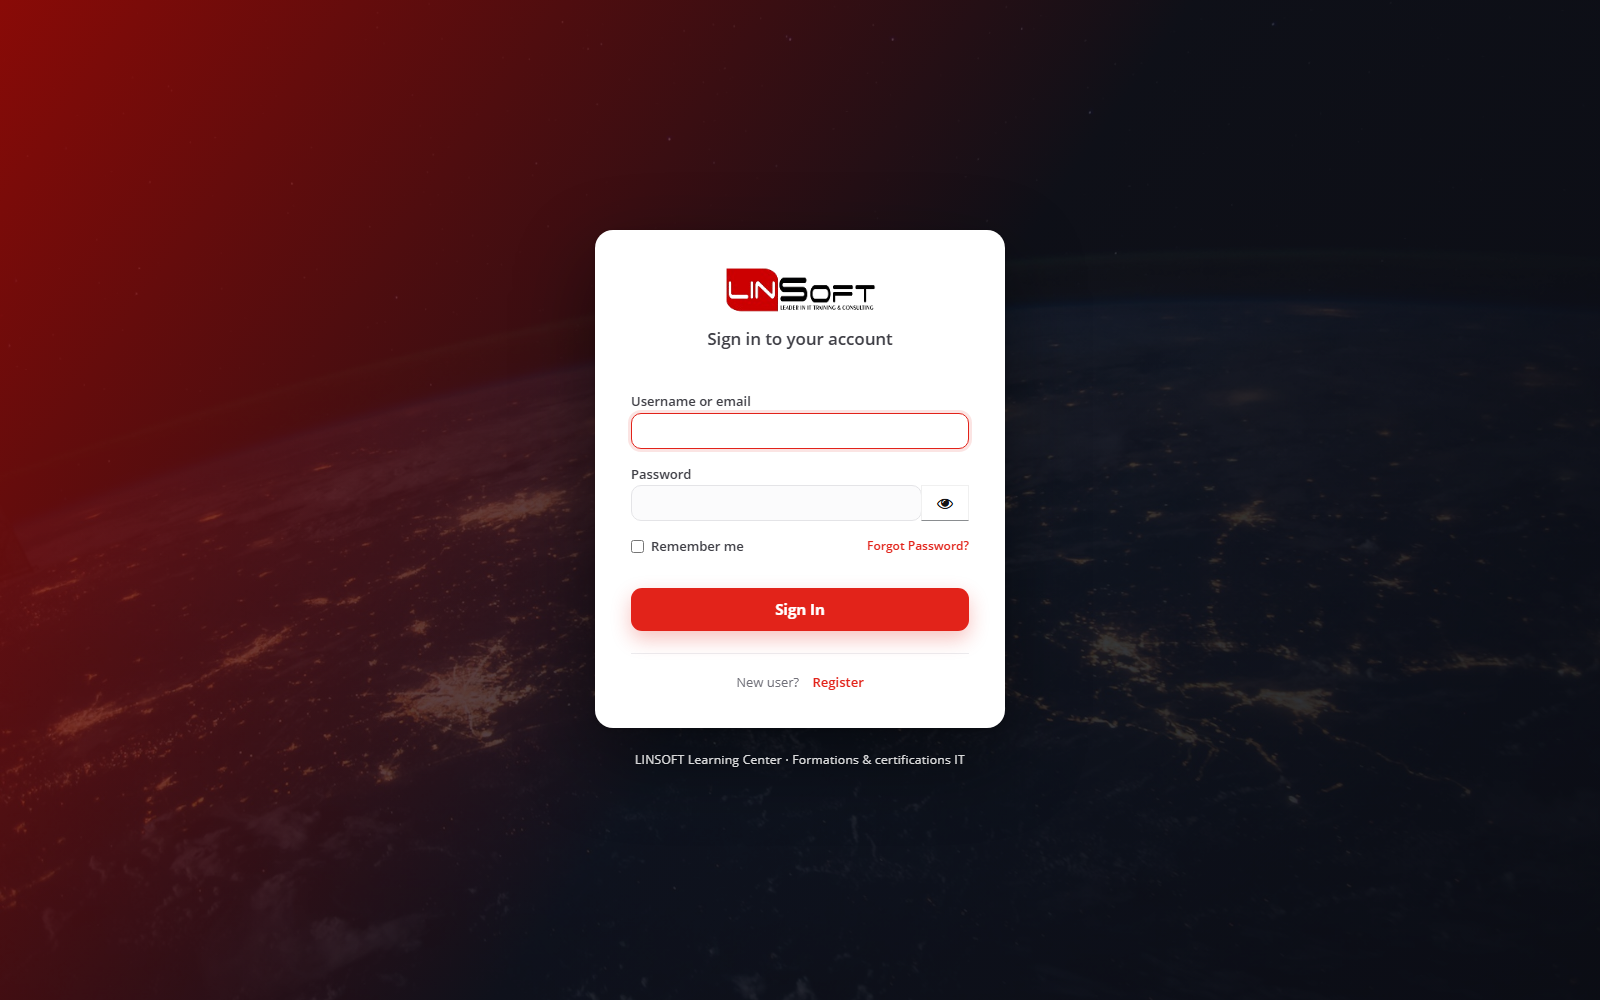
\includegraphics[width=0.92\textwidth]{captures/02-connexion-keycloak.png}
  \caption{Authentification déléguée à Keycloak, traversée automatiquement par les tests}
  \label{fig:e2e-login}
\end{figure}

Les scénarios couvrent l'authentification de chaque rôle, le rejet d'identifiants
invalides, et surtout le \textbf{cloisonnement} : un participant qui saisit l'adresse de
la console d'administration est détourné, un formateur ne peut pas atteindre la gestion des
certificats.

\begin{figure}[H]\centering
  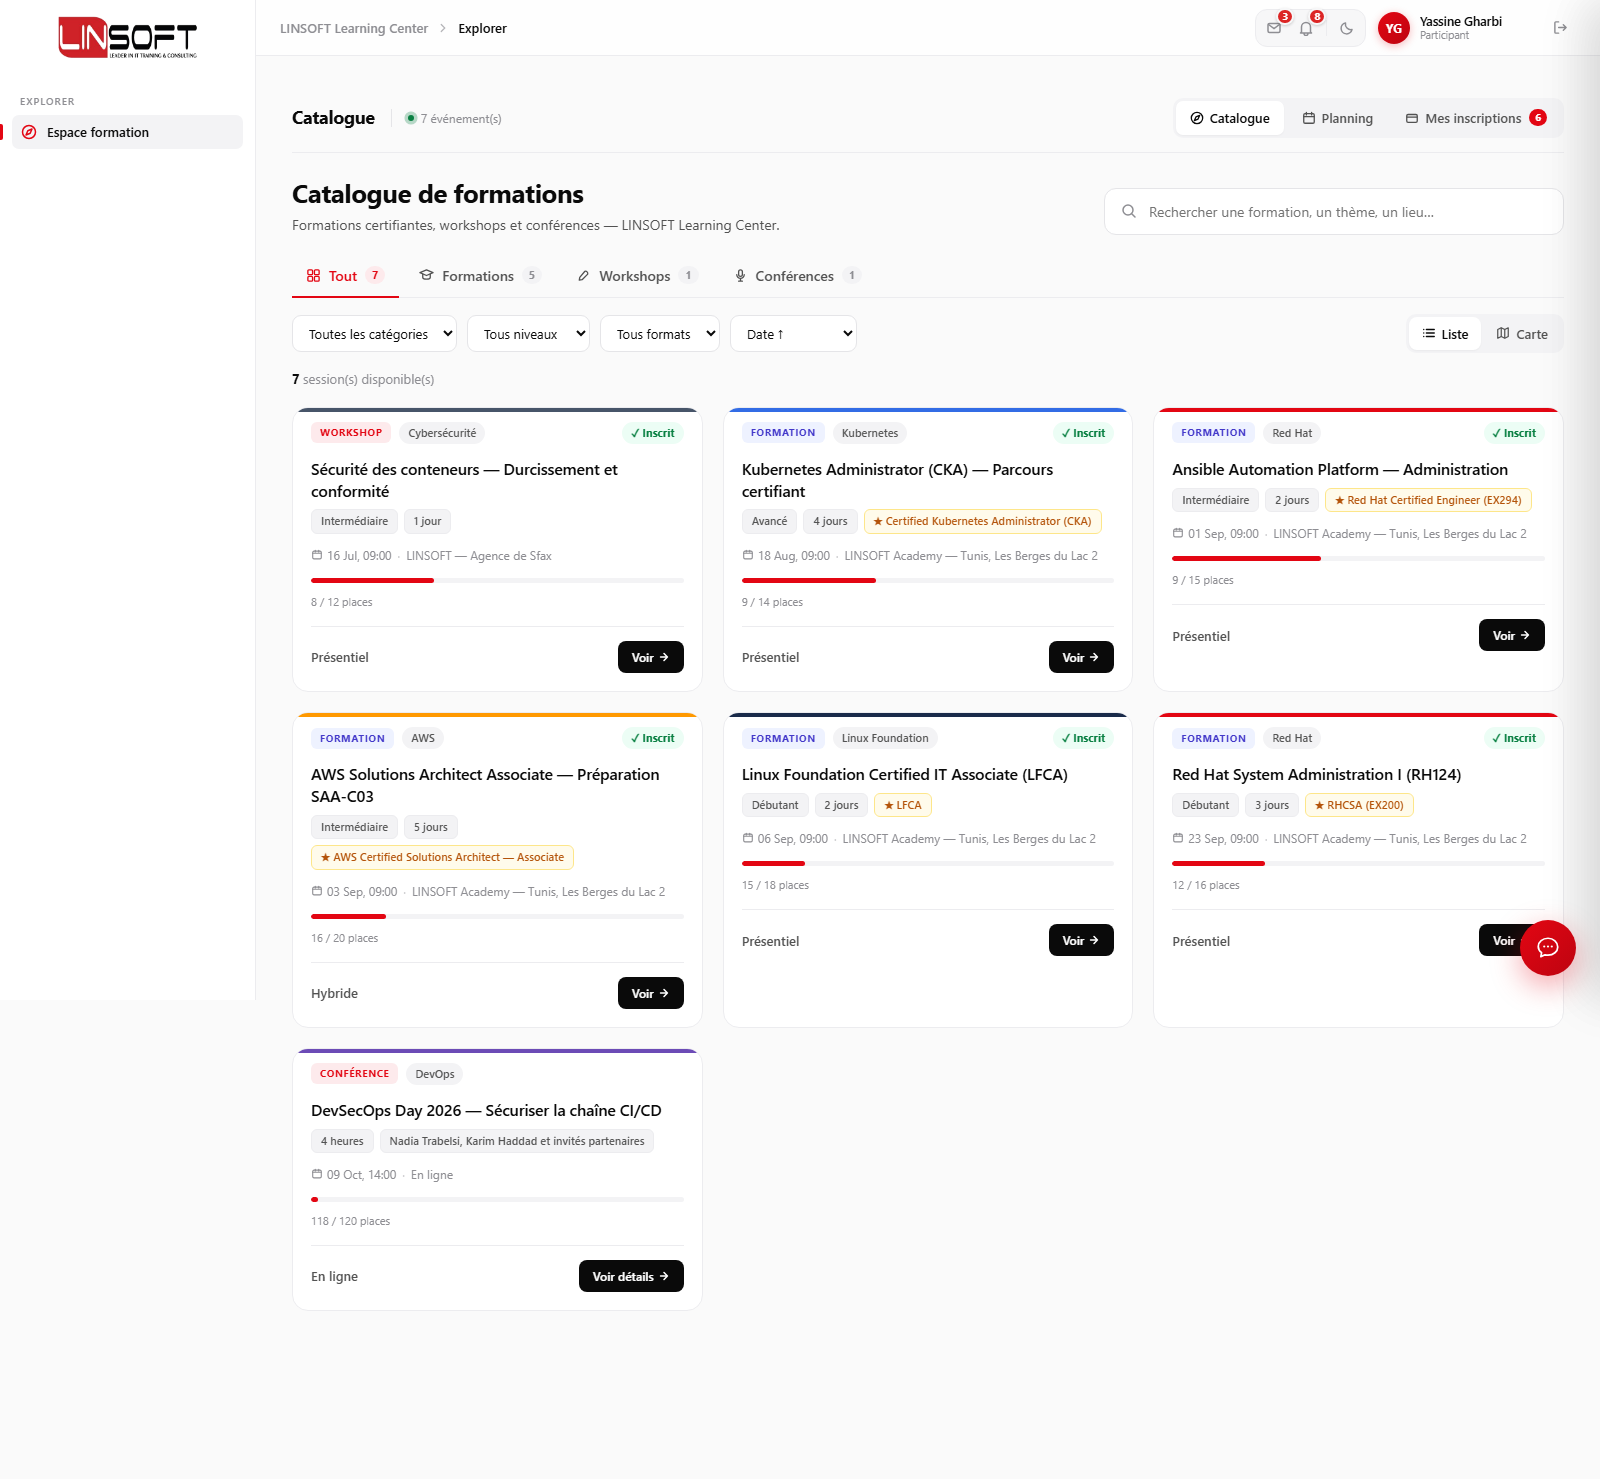
\includegraphics[width=0.92\textwidth]{captures/03-catalogue.png}
  \caption{Catalogue de formations — vue participant}
  \label{fig:devops-catalogue}
\end{figure}

%============================================================================
\section{Qualité du code et couverture}

\subsection{Outils d'analyse}
L'analyse statique (\textbf{Checkstyle} et \textbf{SpotBugs}) est regroupée dans un profil
Maven \texttt{quality}, activé à la demande et en intégration continue. Le jeu de règles
Checkstyle cible délibérément les défauts réels — comparaison de chaînes par
\texttt{==}, \texttt{equals} sans \texttt{hashCode}, blocs \texttt{catch} vides,
\texttt{switch} sans \texttt{default} — plutôt que la mise en forme : un jeu de règles trop
bavard finit systématiquement désactivé.

\subsection{Couverture mesurée}
\textbf{JaCoCo} produit des rapports HTML et XML par module. Le seuil est vérifié à chaque
\texttt{mvn verify} et fait échouer le build s'il n'est pas atteint.

\begin{table}[H]\centering\renewcommand{\arraystretch}{1.25}
\begin{tabular}{|p{5.5cm}|p{3cm}|}\hline
\rowcolor{gray!15}\textbf{Module} & \textbf{Couverture} \\ \hline
\texttt{feedback-service} & 78~\% \\ \hline
\texttt{notification-service} & 74~\% \\ \hline
\texttt{ticket-service} & 71~\% \\ \hline
\texttt{registration-service} & 61~\% \\ \hline
\texttt{event-service} & 53~\% \\ \hline
\texttt{ai-service} & 42~\% \\ \hline
\texttt{user-service} & 41~\% \\ \hline
\end{tabular}
\caption{Couverture des instructions, hors configuration, entités et DTO}\label{tab:couverture}
\end{table}

Le seuil a été relevé progressivement (0~\%, puis 25~\%, 30~\% et enfin 40~\%) au fur et à
mesure de l'écriture des tests. Ce choix est délibéré : un seuil ambitieux fixé d'emblée
aurait été inatteignable et n'aurait produit qu'une chose, sa propre désactivation. Le
seuil joue ainsi le rôle d'un \emph{cliquet anti-régression} plutôt que d'un objectif
décoratif. Son caractère réellement bloquant a été vérifié en le forçant temporairement à
90~\%, ce qui provoque bien l'échec du build.

%============================================================================
\section{Conteneurisation}

Chacun des onze composants dispose de son image. Les images backend reposent sur
\texttt{eclipse-temurin:17-jre-alpine} et appliquent \texttt{chgrp -R 0 /app}, condition
nécessaire sur OpenShift, qui exécute les conteneurs avec un identifiant utilisateur
aléatoire appartenant au groupe~0. Le frontend est construit en deux étapes
(\texttt{node:20-alpine} puis \texttt{nginx-unprivileged}) et s'exécute sans privilèges.

\subsection{Un défaut de conception corrigé}
Les images déclaraient déjà une directive \texttt{HEALTHCHECK} interrogeant
\texttt{/actuator/health}, \textbf{mais sept services sur dix n'embarquaient pas Actuator} :
la sonde recevait une réponse 404. Le fichier \texttt{docker-compose.yml} contournait le
problème par un \texttt{curl -s -o /dev/null || exit 1}, qui \emph{réussit même sur un 404
ou un 401}. Aucune vérification de santé du projet ne prouvait donc quoi que ce soit.
Actuator a été ajouté à tous les services via le POM parent, et les contournements
remplacés par de véritables vérifications.

%============================================================================
\section{Intégration et livraison continues}

\subsection{Architecture du pipeline}
La chaîne est décrite dans \texttt{.github/workflows/ci.yml} et s'exécute sur
\textbf{GitHub Actions} à chaque poussée et à chaque \emph{pull request}.

\begin{table}[H]\centering\renewcommand{\arraystretch}{1.25}
\begin{tabular}{|p{4cm}|p{9.5cm}|}\hline
\rowcolor{gray!15}\textbf{Étape} & \textbf{Contenu} \\ \hline
Tests backend & \texttt{mvn verify} : unitaires, API/sécurité, intégration, couverture \\ \hline
Analyse statique & Checkstyle et SpotBugs \\ \hline
Tests frontend & Vitest puis build de production \\ \hline
Images Docker & Onze images construites en parallèle \\ \hline
Analyse de sécurité & Trivy, vulnérabilités critiques et élevées \\ \hline
Publication & Registre GHCR, branche principale uniquement \\ \hline
Tests E2E & Plateforme complète démarrée, jeu de données semé, Playwright \\ \hline
\end{tabular}
\caption{Étapes de la chaîne d'intégration continue}\label{tab:pipeline}
\end{table}

\subsection{Choix : ne pas compiler dans les images}
Les fichiers \texttt{Dockerfile} du backend copient une archive JAR déjà construite plutôt
que de la compiler. Une construction multi-étapes par service recompilerait dix fois le même
réacteur Maven, pour un résultat identique. Le réacteur est donc construit \textbf{une
seule fois}, les archives circulent en artefact entre les étapes, et chaque image est
assemblée à partir du binaire validé : l'artefact testé et l'artefact publié sont ainsi le
même objet.

\subsection{Garde-fou contre les faux positifs}
Une étape vérifie explicitement qu'\textbf{aucun test d'intégration n'a été ignoré} alors
que Docker était disponible. Sans ce contrôle, un environnement dépourvu de Docker
produirait un pipeline vert trompeur, puisque les tests Testcontainers s'ignorent
automatiquement en l'absence de démon.

\subsection{Deux défauts révélés par les premières exécutions}
Aucun des deux n'était détectable en local, ce qui illustre précisément l'apport d'une
chaîne d'intégration continue.

\begin{enumerate}
  \item \textbf{Référence d'action non résolue.} Les onze tâches de construction d'images
        échouaient à l'étape « Set up job », c'est-à-dire \emph{avant} leur première
        instruction. Les étiquettes du dépôt \texttt{trivy-action} sont préfixées par
        \texttt{v} : la référence \texttt{@0.28.0} n'existait pas. GitHub Actions résout les
        actions avant de les exécuter, d'où un échec sans aucune trace dans les étapes.
  \item \textbf{Nom d'image refusé par le registre.} Une fois ce point corrigé, la
        construction, l'analyse Trivy et l'authentification réussissaient, mais la
        publication échouait — symptôme trompeur. Le compte GitHub s'écrit
        \texttt{Medamine009}, avec une majuscule, alors que GHCR n'accepte que des noms
        d'image en minuscules. Le nom est désormais normalisé avant usage.
\end{enumerate}

%============================================================================
\section{Supervision et observabilité}

\subsection{Points de mesure}
Tous les services exposent, via Actuator et Micrometer, un agrégat de santé, des sondes
distinctes de \emph{liveness} et de \emph{readiness}, ainsi que leurs métriques au format
Prometheus. L'exposition est volontairement restreinte aux points réellement utilisés :
\texttt{env}, \texttt{beans} et \texttt{heapdump} restent fermés.

\subsection{Collecte et visualisation}
Prometheus interroge les dix services toutes les quinze secondes ; Grafana en propose la
lecture. L'ensemble est placé derrière un profil Docker Compose afin de ne pas alourdir le
démarrage courant de la plateforme.

\begin{figure}[H]\centering
  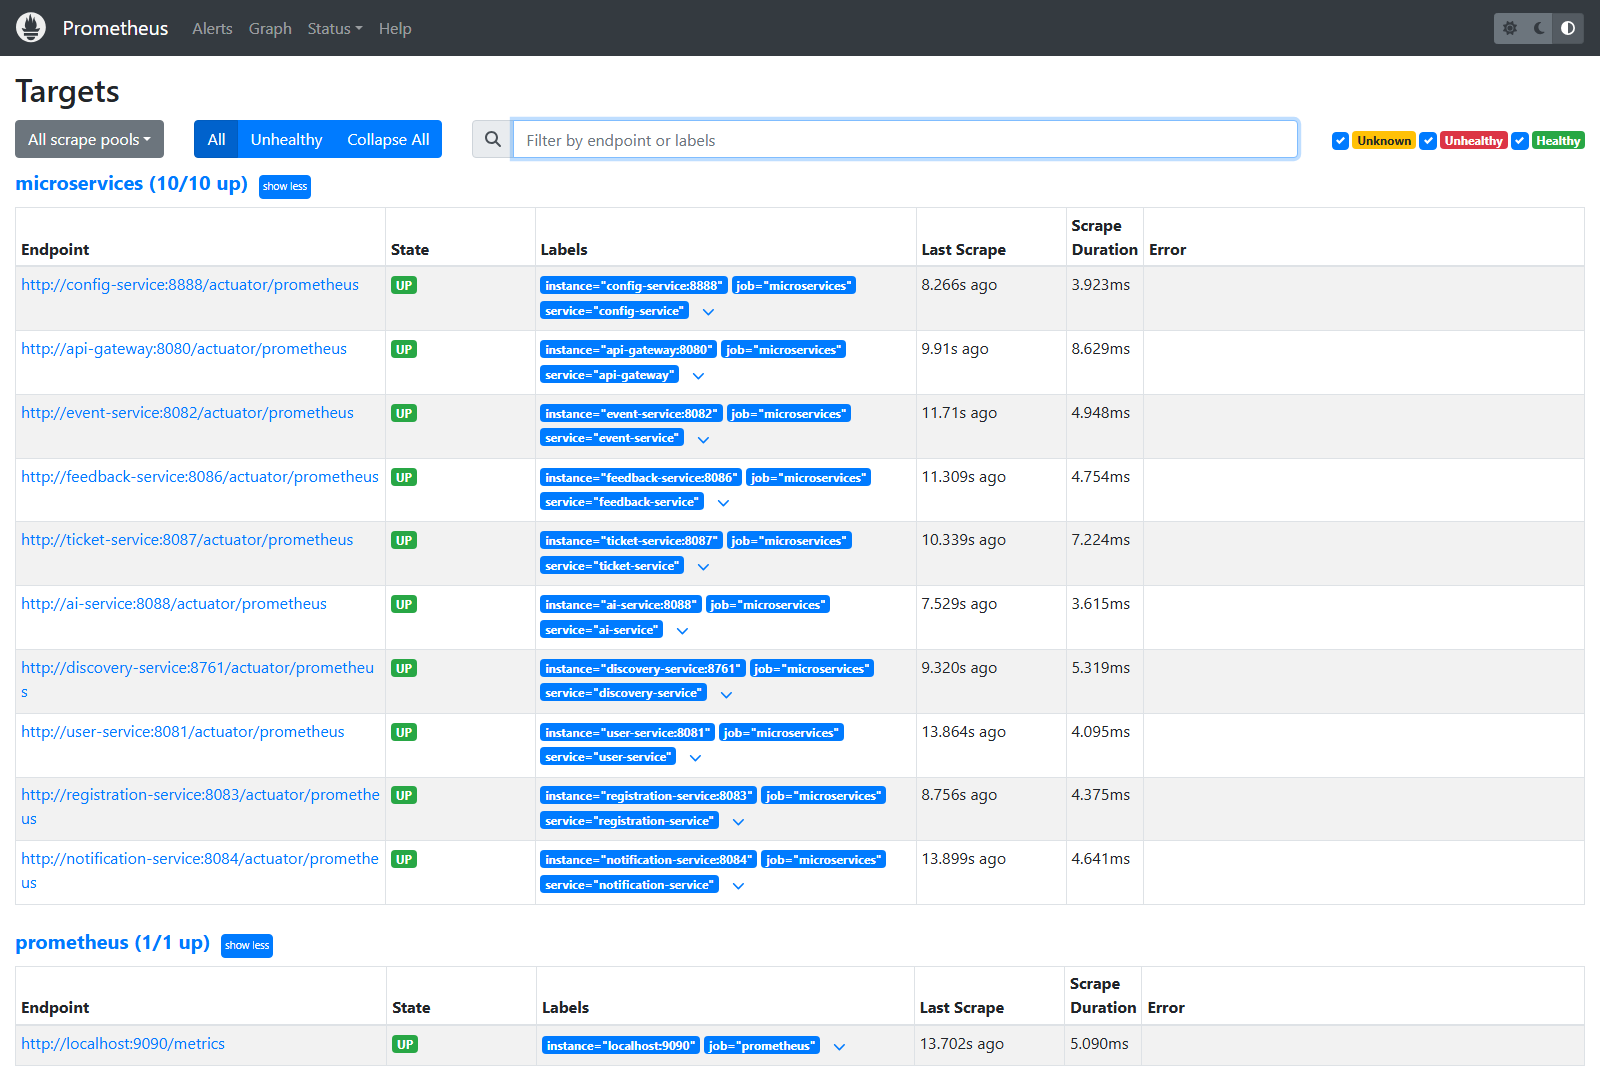
\includegraphics[width=0.92\textwidth]{captures/08-prometheus-cibles.png}
  \caption{Cibles Prometheus : les dix microservices interrogés avec succès}
  \label{fig:prometheus}
\end{figure}

\begin{figure}[H]\centering
  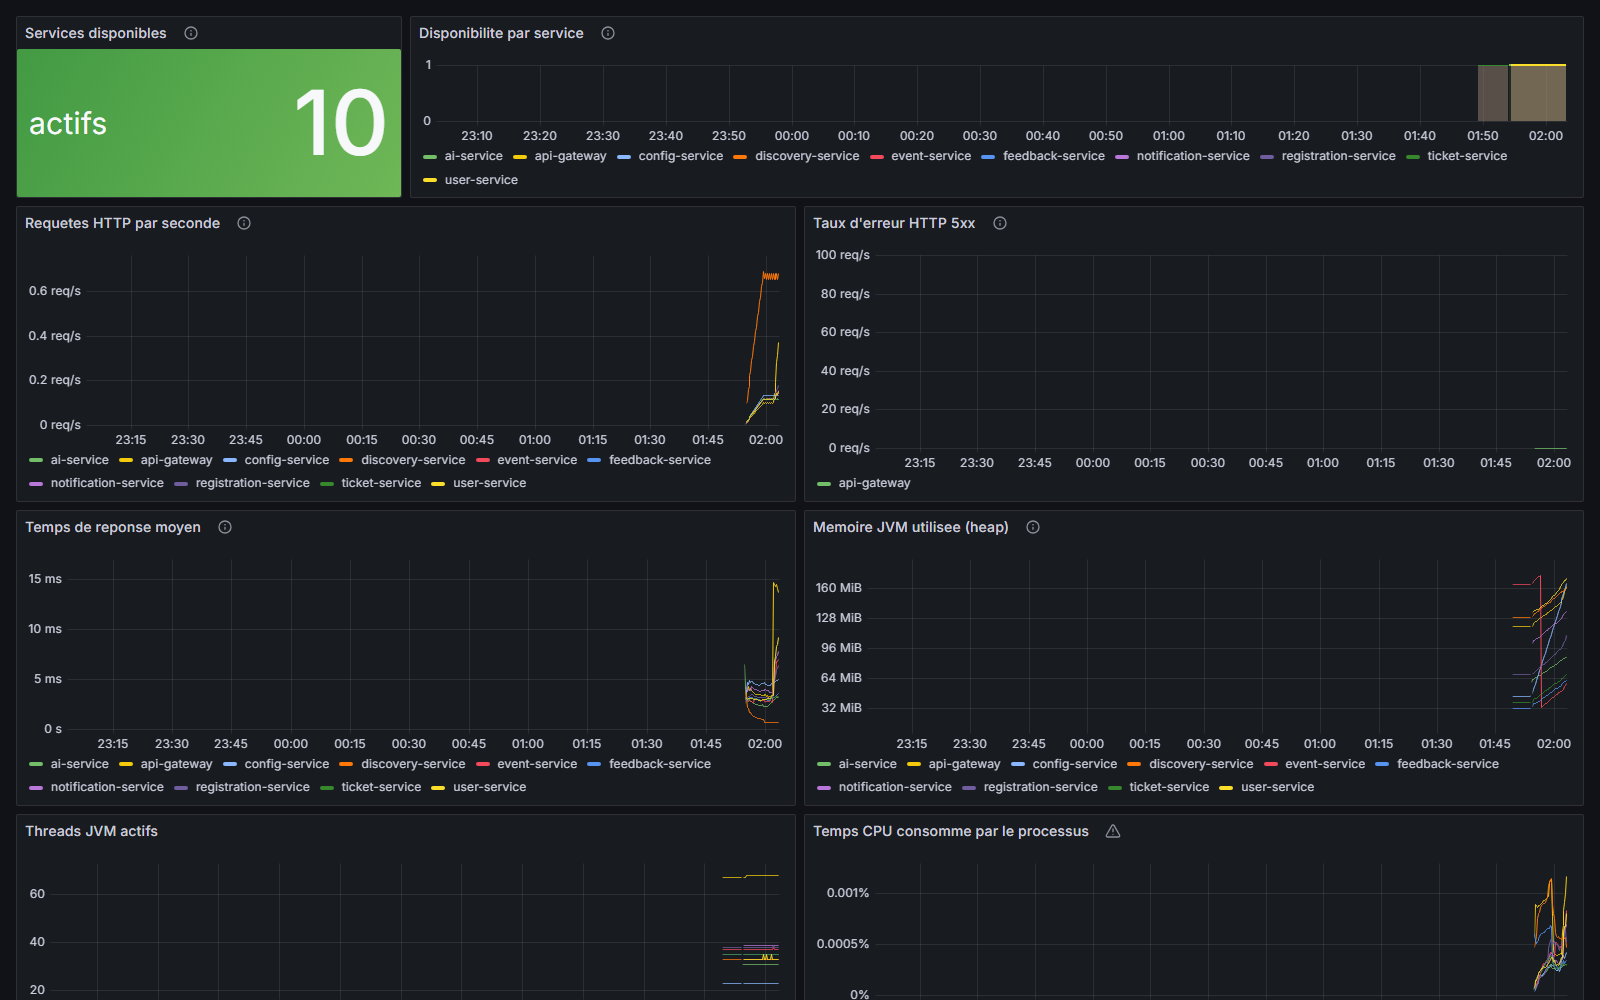
\includegraphics[width=\textwidth]{captures/09-grafana-plateforme.png}
  \caption{Tableau de bord Grafana : disponibilité, charge, temps de réponse et mémoire}
  \label{fig:grafana}
\end{figure}

Chaque série porte une étiquette \texttt{application} apposée par Micrometer ; sans elle,
les séries des dix services seraient indistinguables.

\begin{figure}[H]\centering
  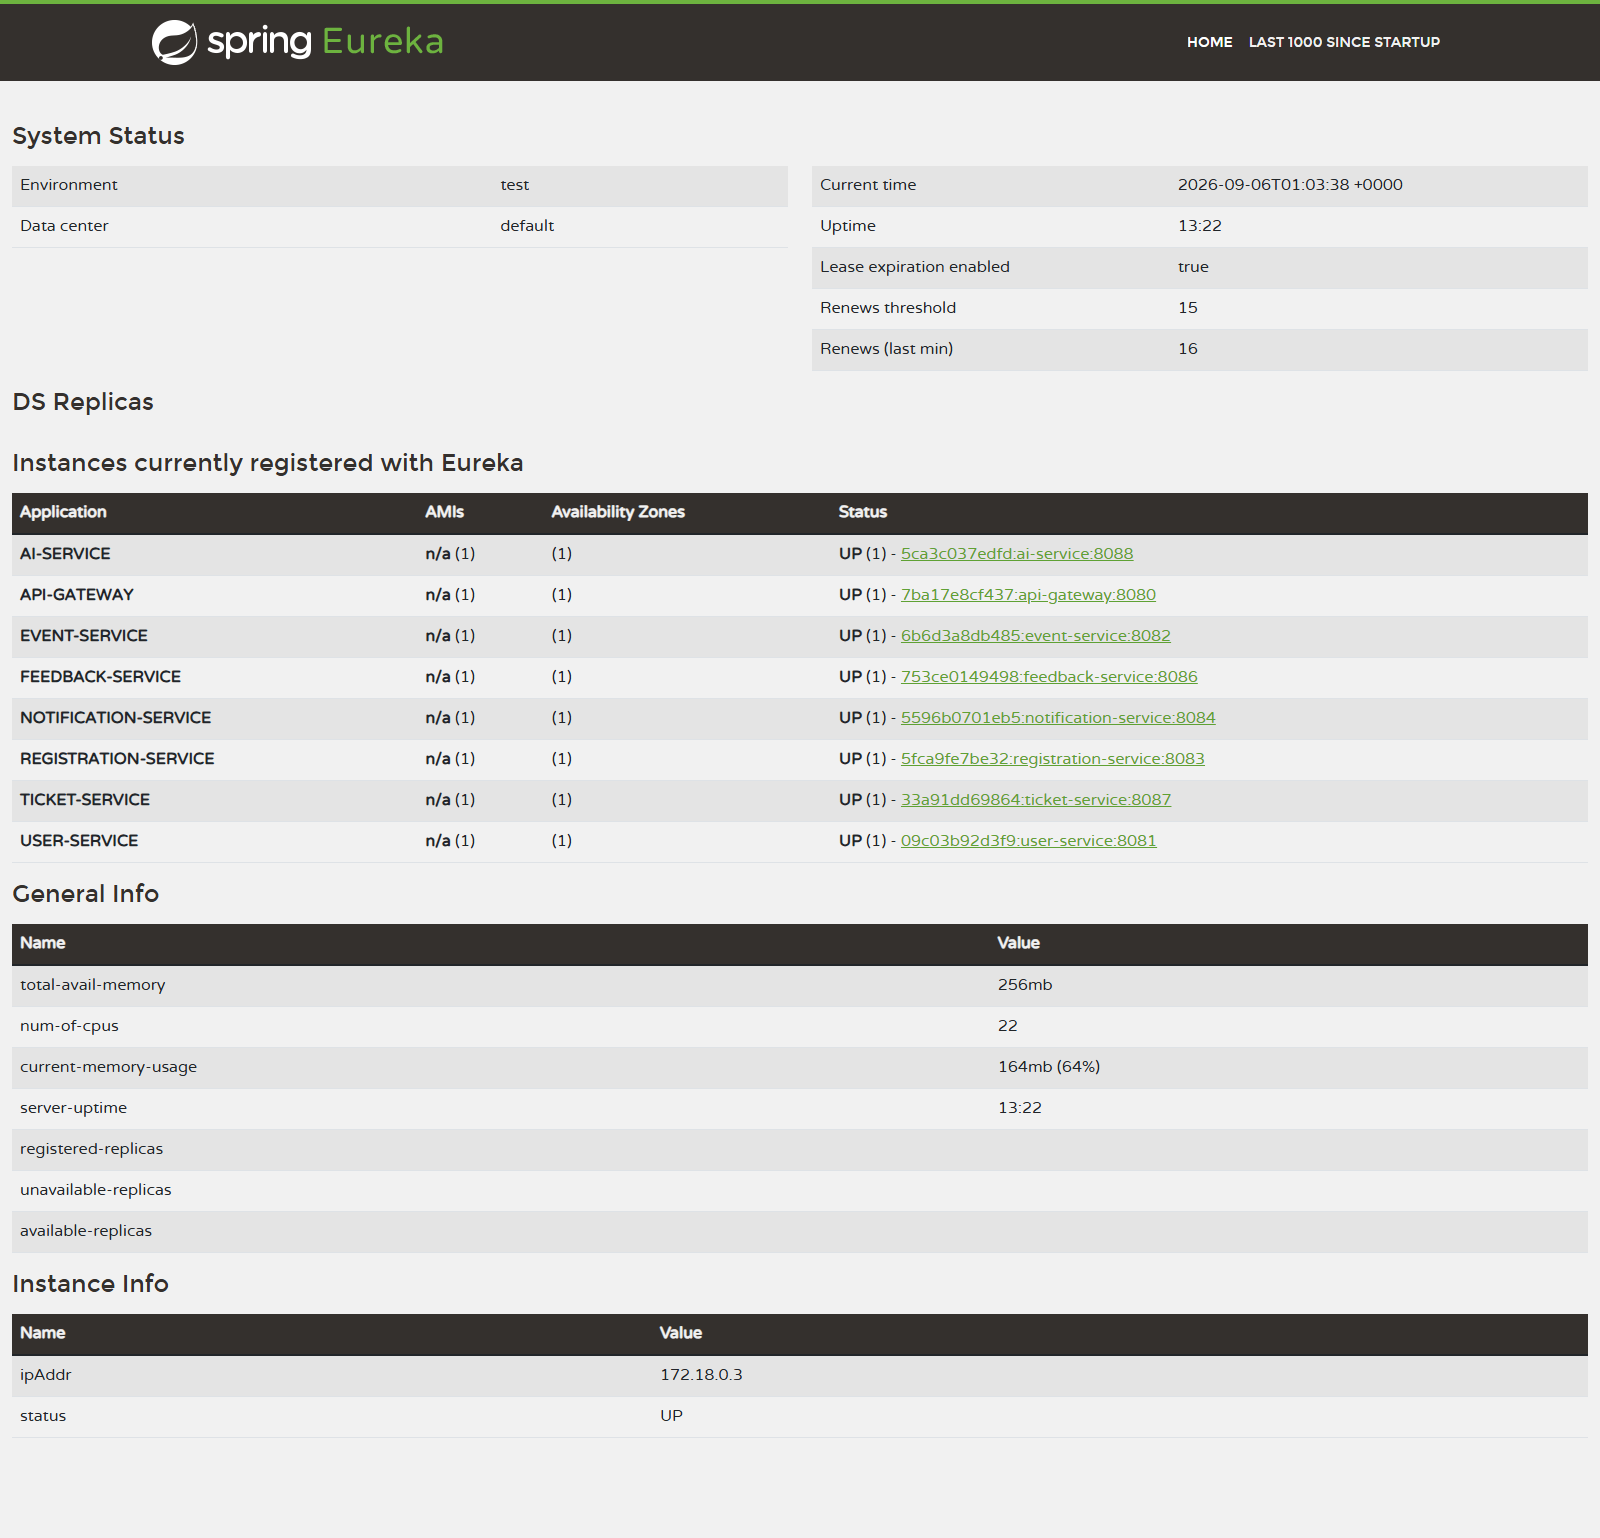
\includegraphics[width=0.92\textwidth]{captures/11-eureka.png}
  \caption{Registre Eureka : services enregistrés et découverte dynamique}
  \label{fig:eureka}
\end{figure}

\begin{figure}[H]\centering
  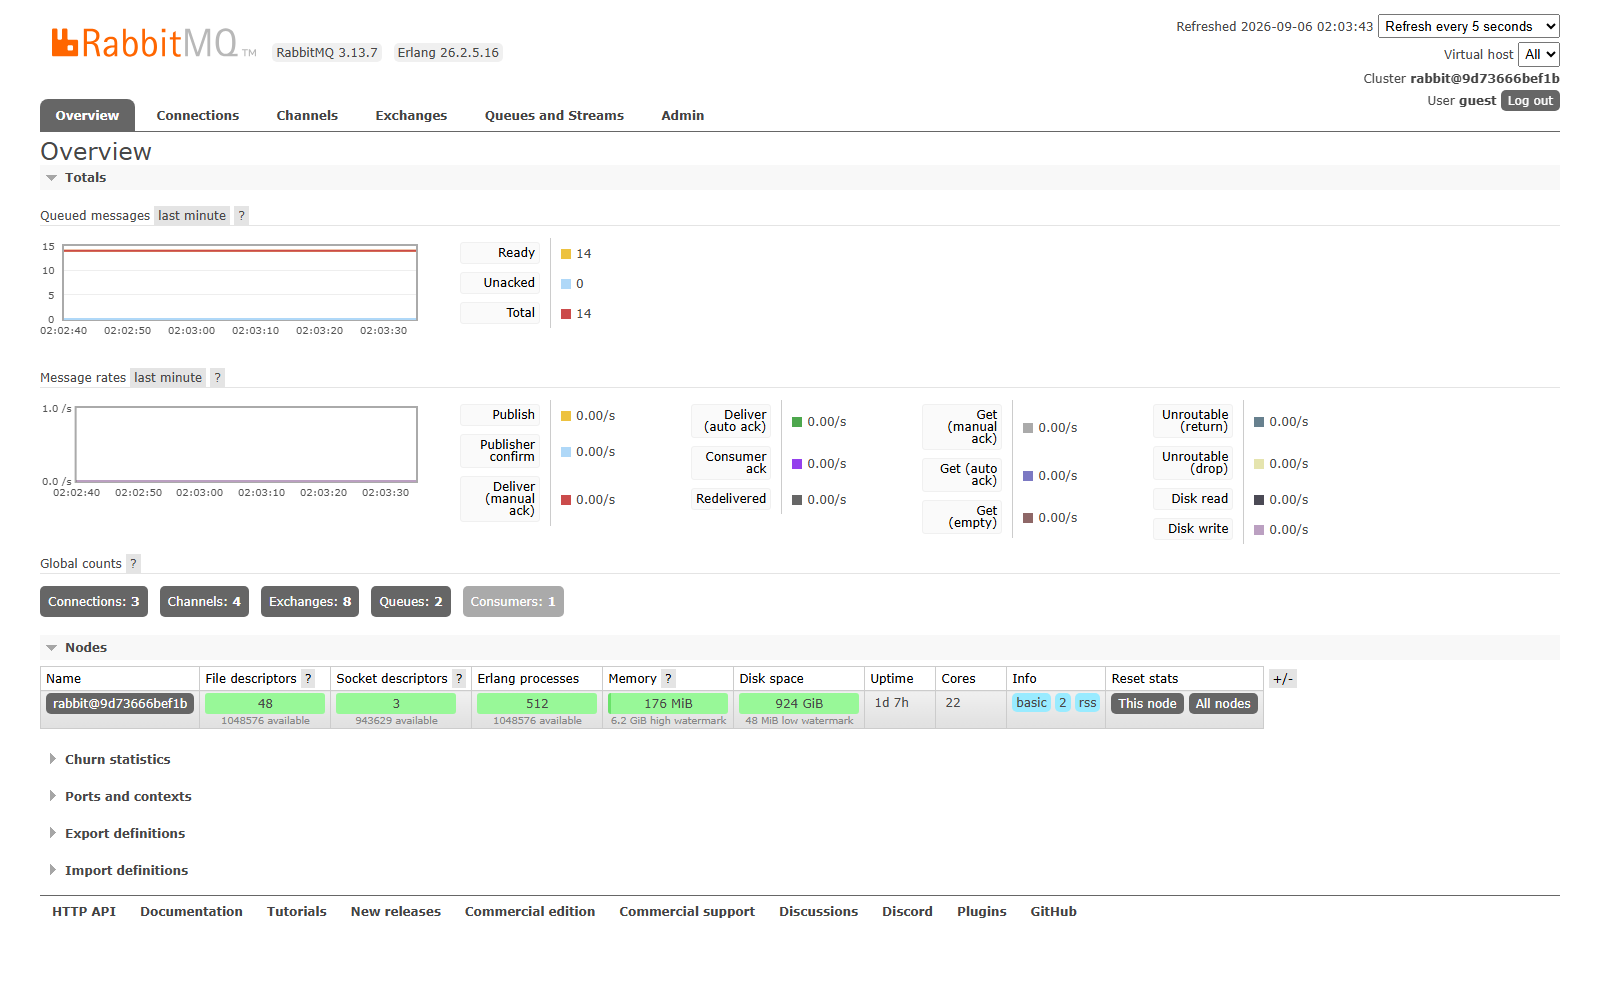
\includegraphics[width=0.92\textwidth]{captures/12-rabbitmq.png}
  \caption{Console RabbitMQ : file de notifications et débit des messages}
  \label{fig:rabbitmq}
\end{figure}

%============================================================================
\section{Sécurité de la chaîne}

\begin{itemize}
  \item \textbf{Analyse des images} : Trivy inspecte chaque image et remonte les
        vulnérabilités critiques et élevées dans l'onglet \emph{Security} du dépôt.
  \item \textbf{Aucun secret versionné} : la publication utilise le jeton fourni par la
        plateforme. Le fichier \texttt{.env} est exclu du dépôt et accompagné d'un modèle
        \texttt{.env.example}.
  \item \textbf{Secrets de déploiement} : un script \texttt{create-secrets.sh} génère des
        mots de passe aléatoires via \texttt{oc create secret}, de sorte qu'aucune valeur
        réelle ne transite par Git.
\end{itemize}

%============================================================================
\section{Illustrations du parcours fonctionnel}

Les captures suivantes montrent le résultat obtenu sur les fonctionnalités les plus
structurantes, avec le jeu de données de démonstration.

\begin{figure}[H]\centering
  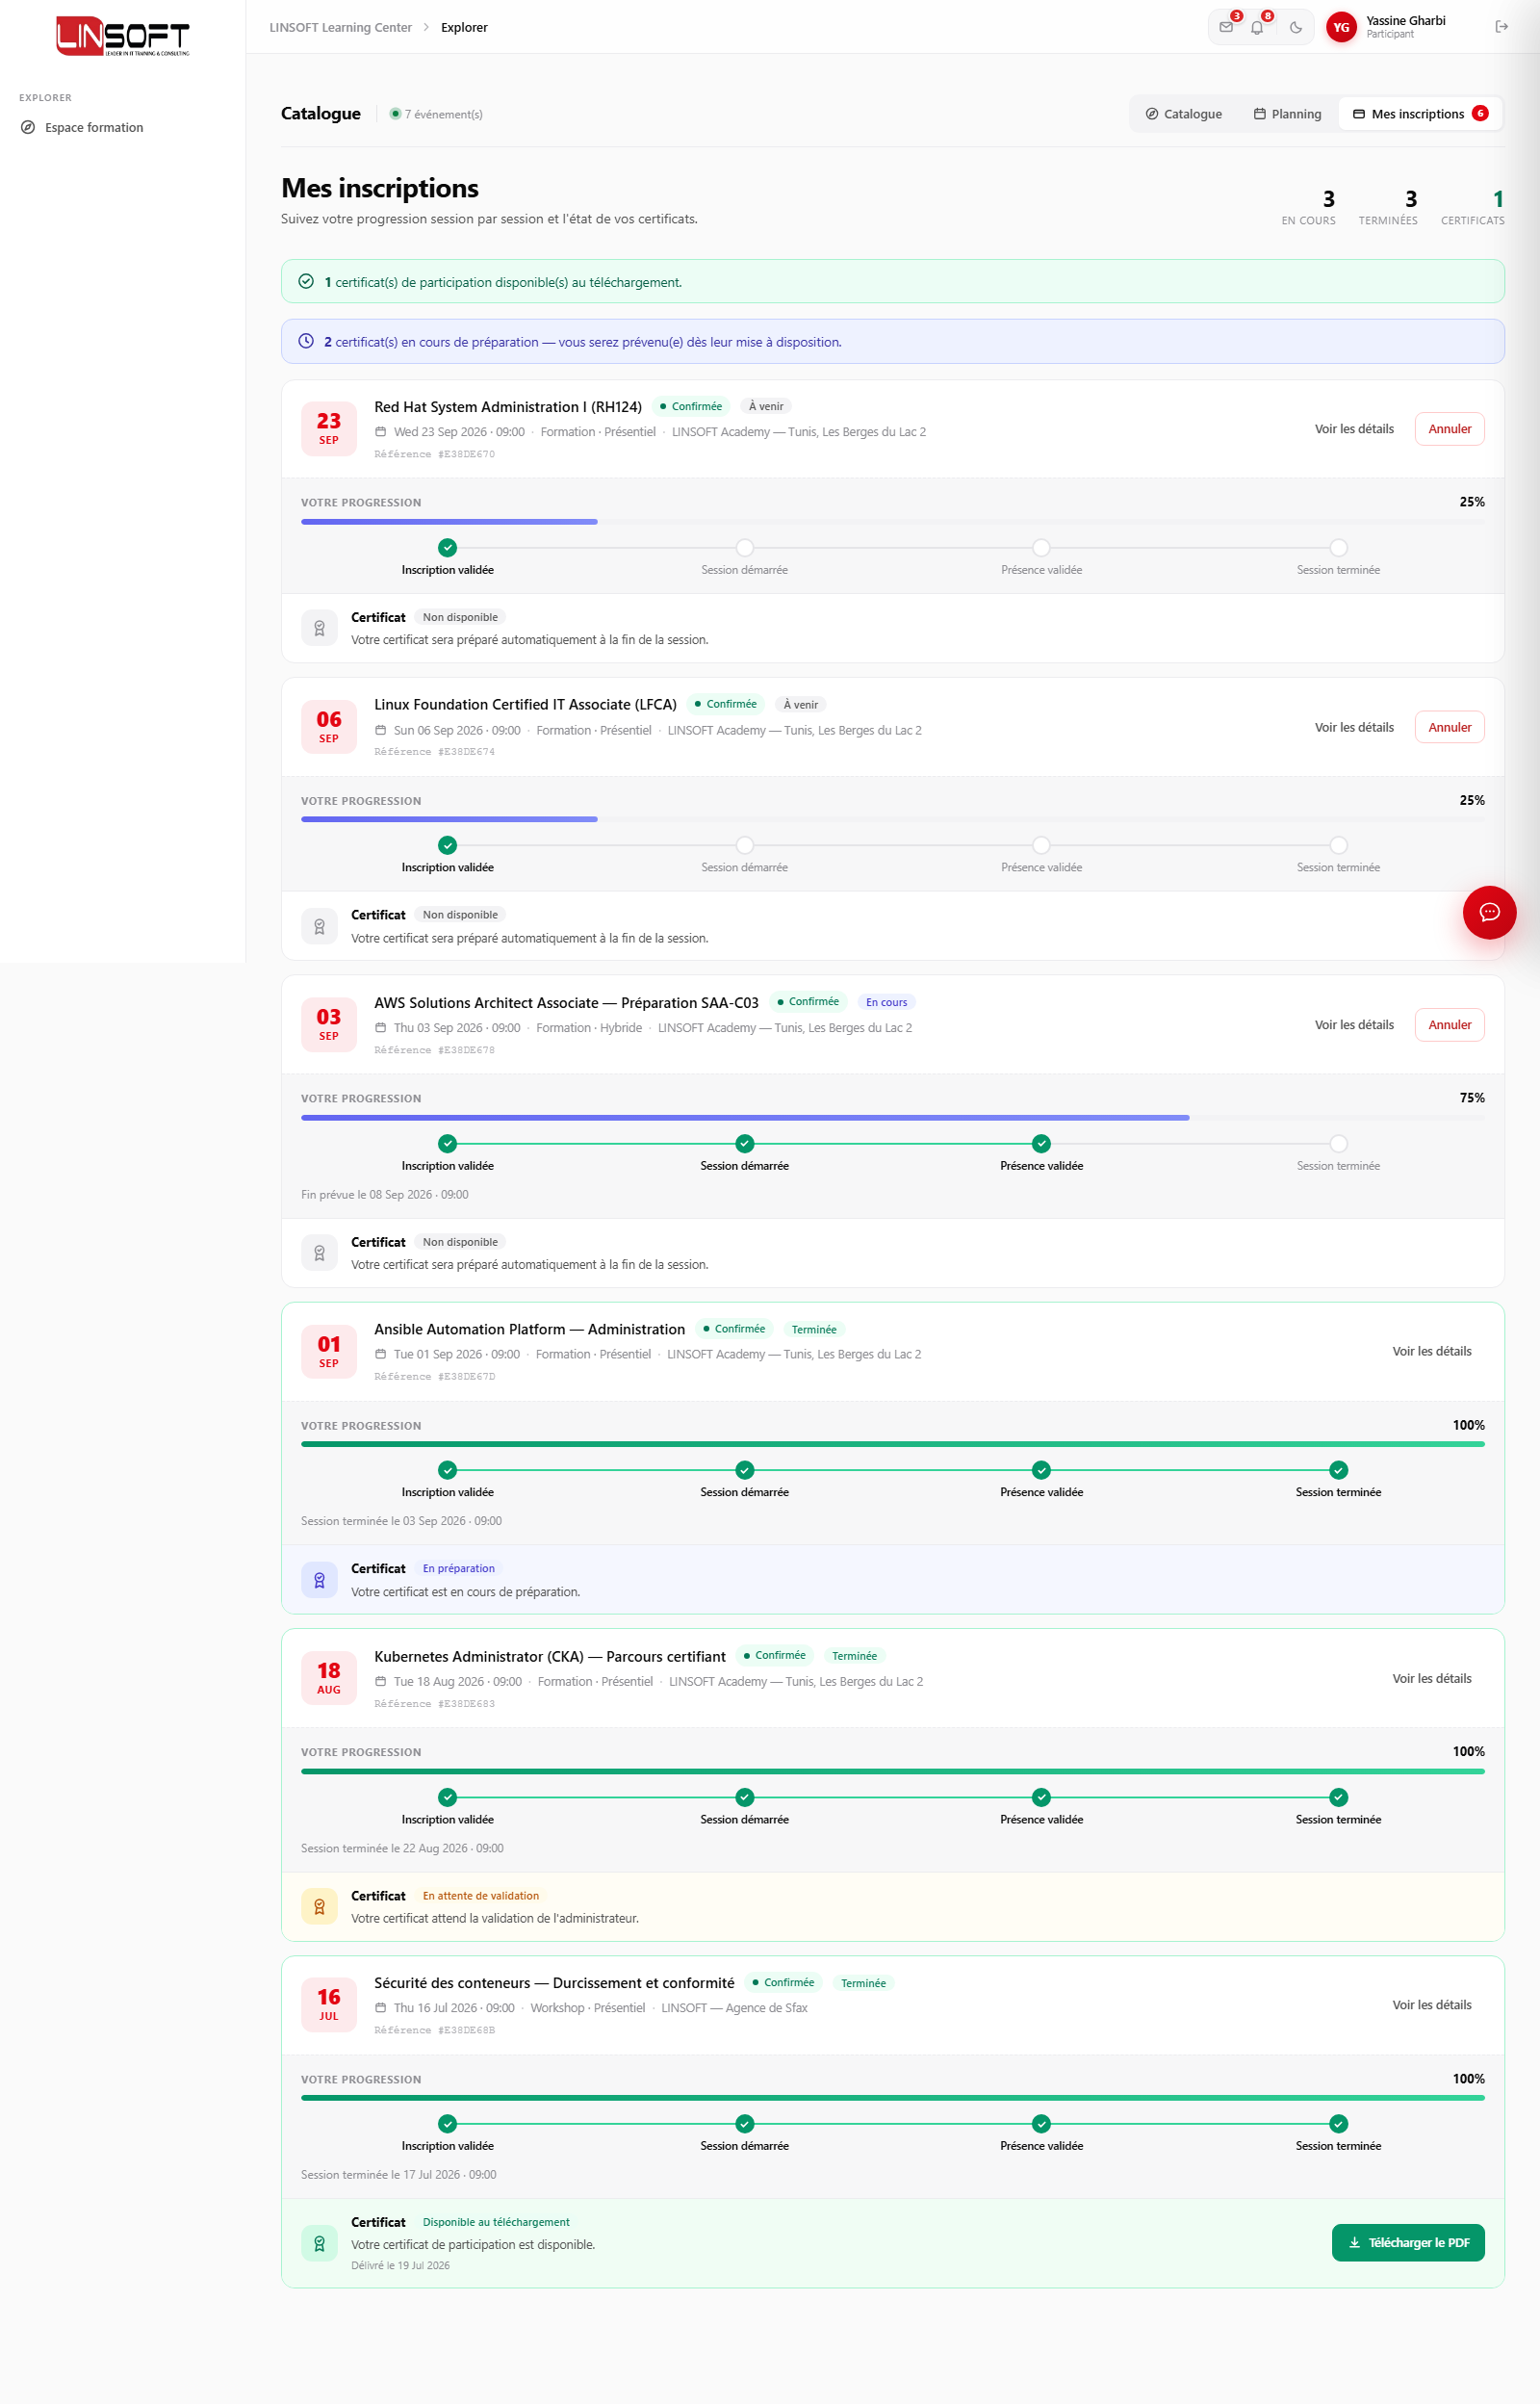
\includegraphics[width=0.85\textwidth]{captures/04-suivi-certificats.png}
  \caption{Suivi de participation : progression par jalons et cycle de vie du certificat}
  \label{fig:suivi}
\end{figure}

Cette vue rassemble les cinq états du parcours : session à venir (certificat non
disponible), session en cours avec progression intermédiaire, puis session terminée avec un
certificat successivement \emph{en préparation}, \emph{en attente de validation} et enfin
\emph{disponible au téléchargement}.

\begin{figure}[H]\centering
  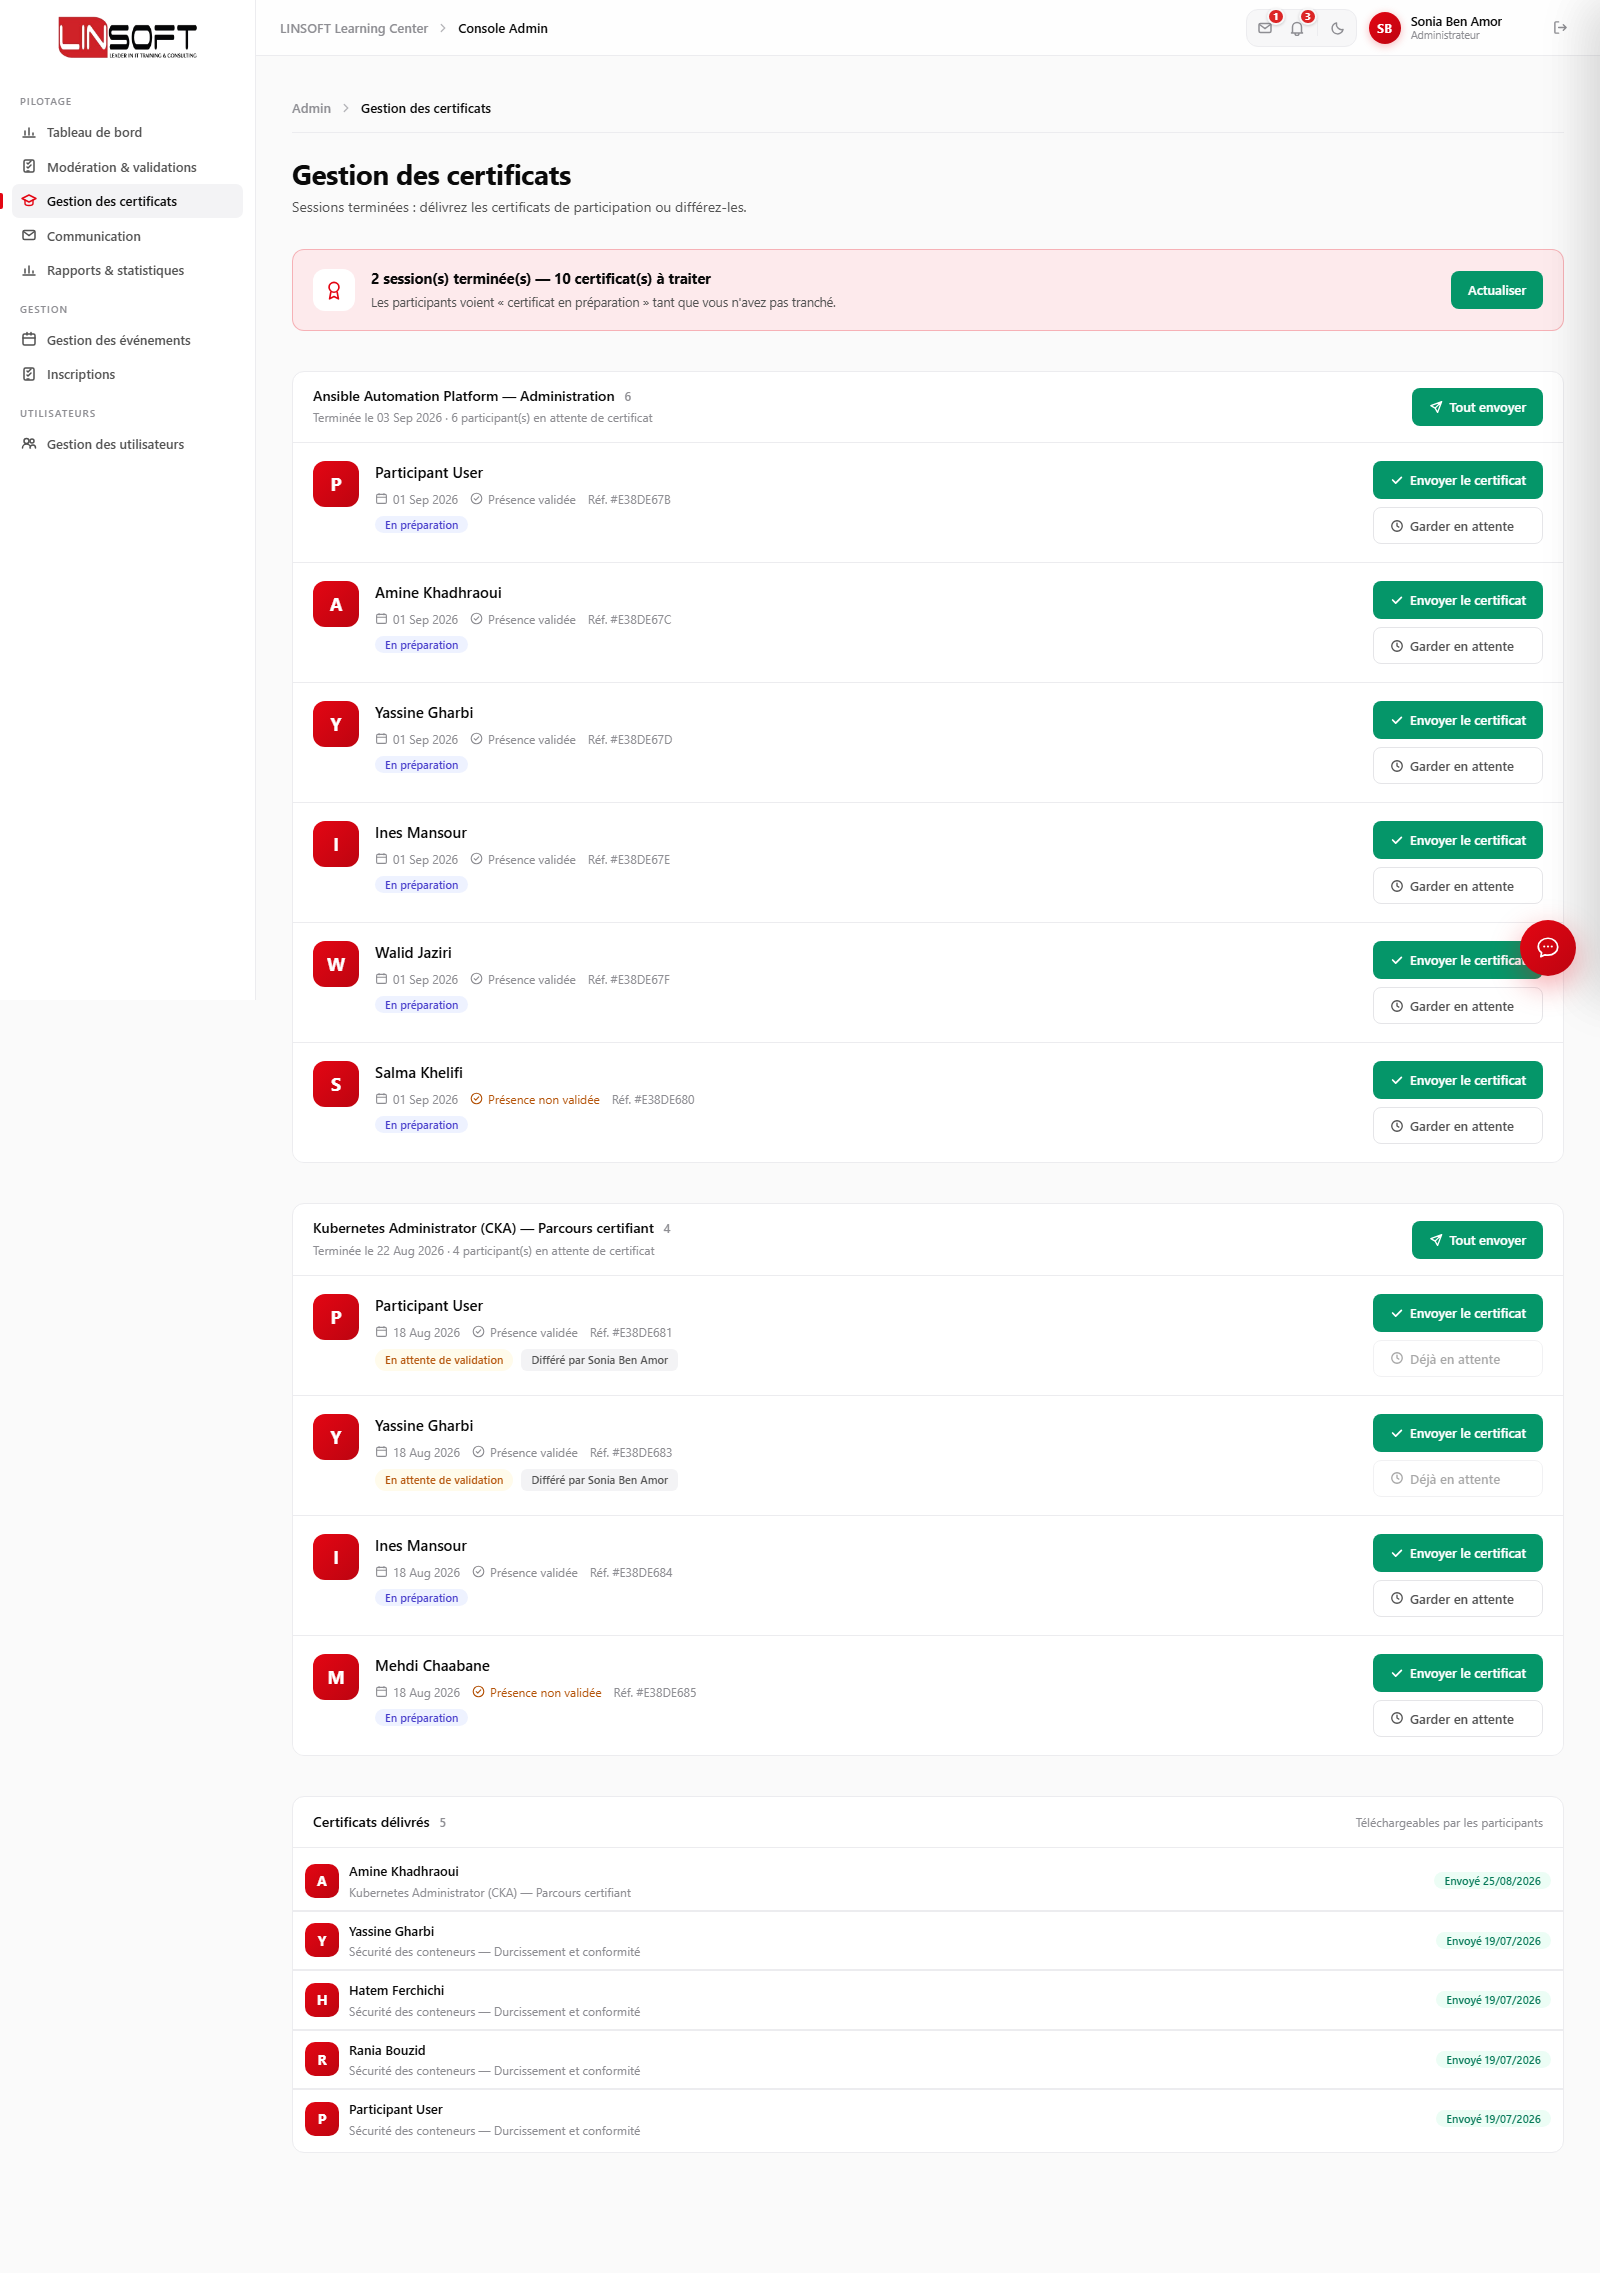
\includegraphics[width=0.85\textwidth]{captures/06-gestion-certificats.png}
  \caption{Console d'administration : file des certificats à délivrer, groupée par session}
  \label{fig:certificats-admin}
\end{figure}

\begin{figure}[H]\centering
  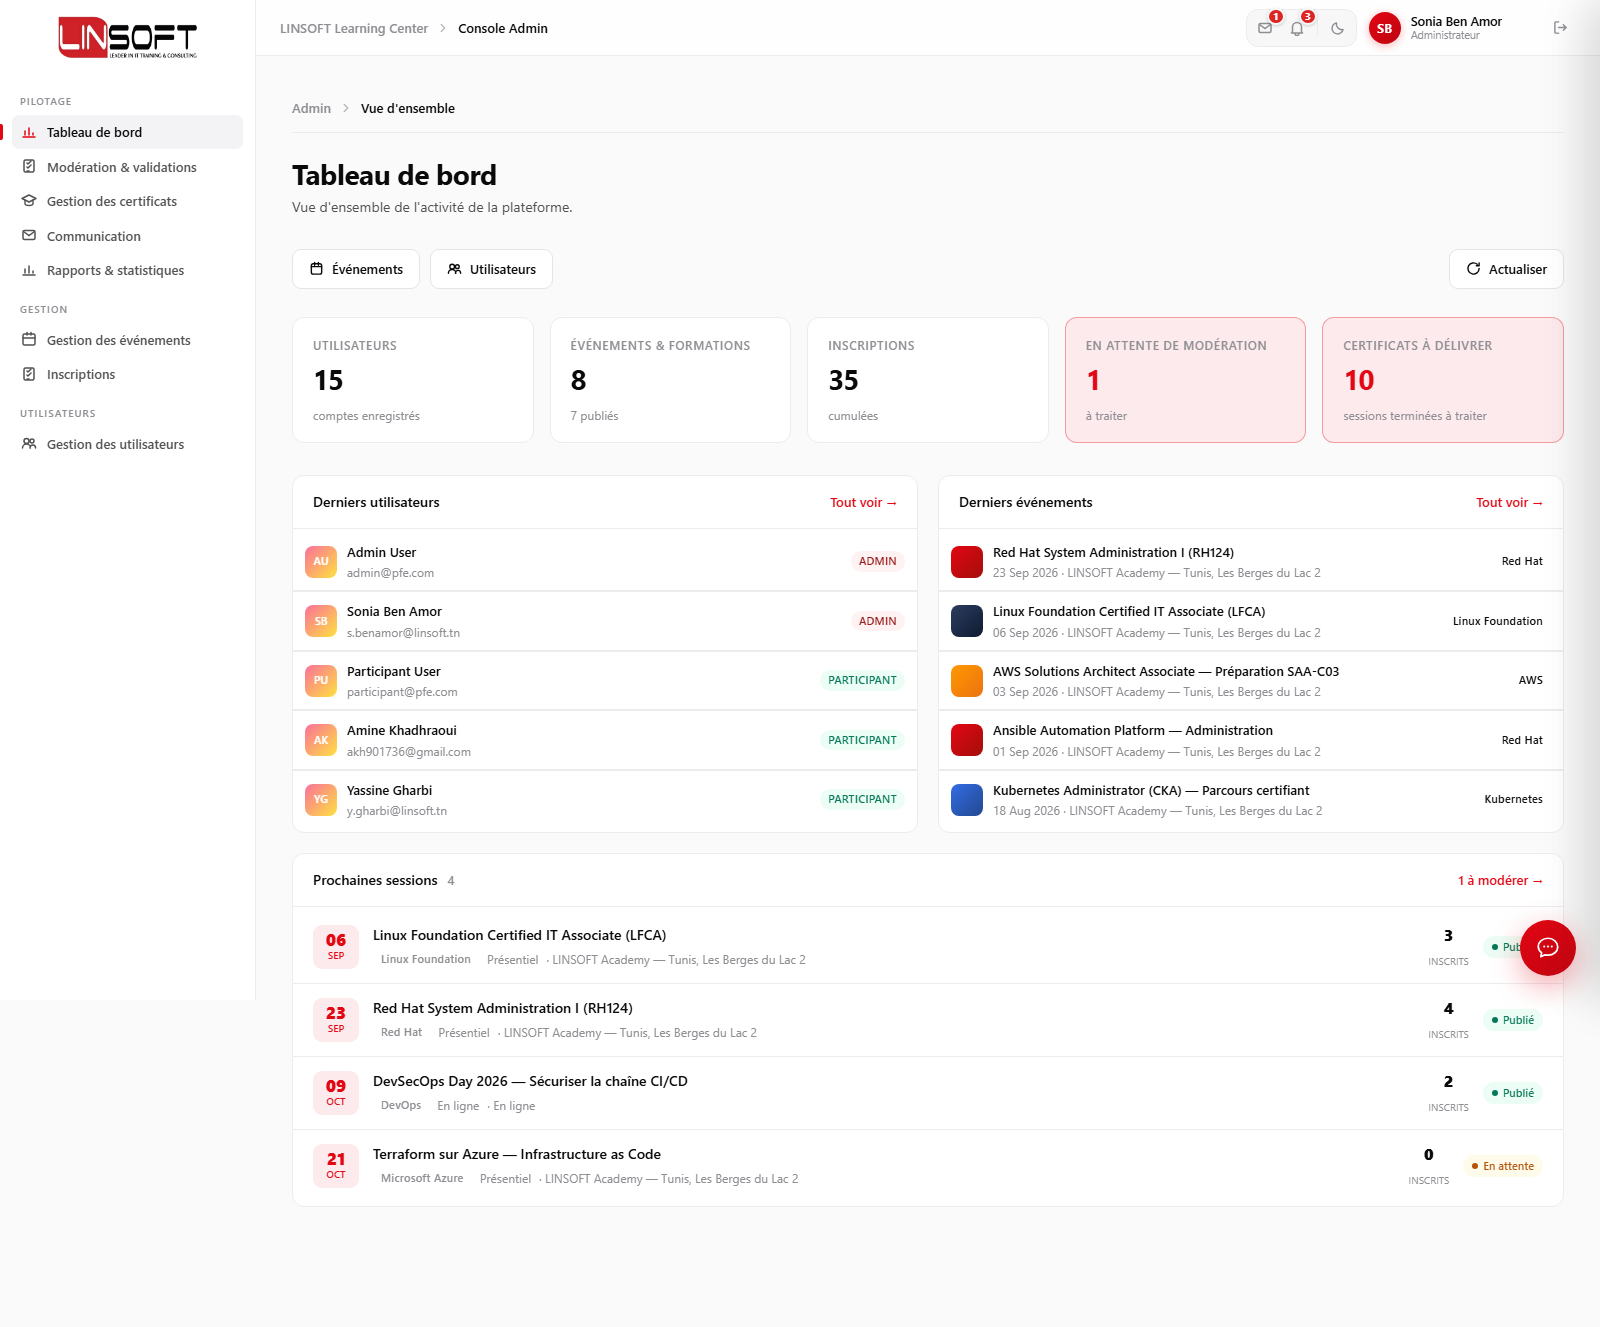
\includegraphics[width=0.92\textwidth]{captures/05-admin-dashboard.png}
  \caption{Tableau de bord administrateur et indicateurs de la plateforme}
  \label{fig:admin}
\end{figure}

\begin{figure}[H]\centering
  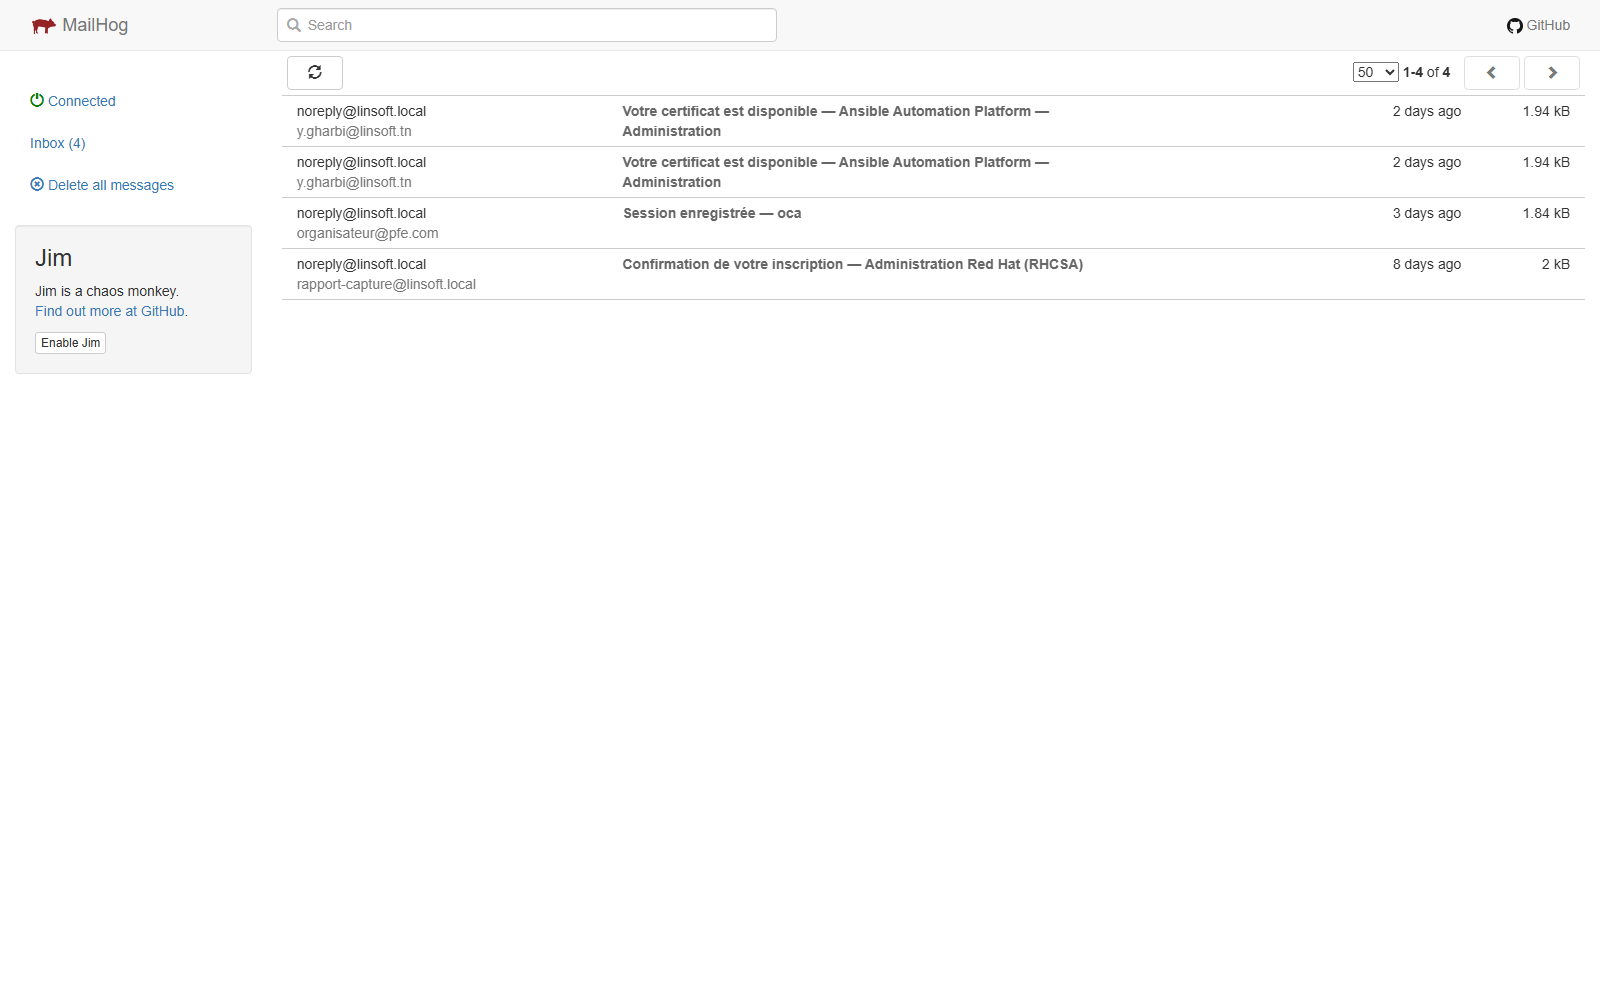
\includegraphics[width=0.92\textwidth]{captures/10-mailhog.png}
  \caption{Courriels émis par la plateforme, interceptés par MailHog en environnement de test}
  \label{fig:mailhog}
\end{figure}

%============================================================================
\section*{Conclusion}
La démarche présentée dans ce chapitre a fait passer le projet de dix-huit tests sans mesure
de couverture à près de trois cents tests répartis sur quatre niveaux, adossés à une chaîne
d'intégration continue de dix-sept tâches et à un dispositif de supervision opérationnel.
Au-delà des chiffres, cette démarche a démontré sa valeur en révélant des défauts réels et
invisibles autrement : des vérifications de santé qui ne vérifiaient rien, une référence
d'action inexistante, un nom d'image refusé par le registre, et une référence de dossier
identique pour toute une promotion de participants.

%  Les captures référencées se trouvent dans rapport-pfe/captures/
%############################################################################
\chapter{Tests, qualité et démarche DevOps}

\section*{Introduction}
Une plateforme composée de dix microservices ne se valide pas en la parcourant à la main :
le nombre de combinaisons de rôles, d'états et de services rend la vérification manuelle
à la fois incomplète et non reproductible. Ce chapitre présente la stratégie de test mise
en place, les outils de mesure de la qualité, la chaîne d'intégration continue et le
dispositif de supervision. Chaque choix y est justifié par le défaut qu'il permet de
détecter, et les résultats présentés sont ceux réellement obtenus sur la plateforme.

%============================================================================
\section{Stratégie de test}

\subsection{Pyramide de test retenue}
Quatre niveaux de test se répondent, chacun apportant une garantie que les autres ne
peuvent pas fournir.

\begin{table}[H]\centering\renewcommand{\arraystretch}{1.3}
\begin{tabular}{|p{3.2cm}|p{5cm}|p{6cm}|}\hline
\rowcolor{gray!15}\textbf{Niveau} & \textbf{Outils} & \textbf{Question à laquelle il répond} \\ \hline
Unitaire & JUnit 5, Mockito & La règle métier est-elle juste ? \\ \hline
API / Sécurité & MockMvc, spring-security-test & L'API applique-t-elle réellement les droits ? \\ \hline
Intégration & Testcontainers (MongoDB) & Le code dialogue-t-il correctement avec une base réelle ? \\ \hline
Bout en bout & Playwright, Chromium & Le parcours utilisateur fonctionne-t-il entièrement ? \\ \hline
\end{tabular}
\caption{Niveaux de test et rôle de chacun}\label{tab:pyramide}
\end{table}

\subsection{Séparation des tests rapides et des tests d'infrastructure}
La convention de nommage pilote l'exécution, configurée une seule fois dans le POM parent :
les classes \texttt{*Test} sont exécutées par Surefire pendant la phase \texttt{test}, les
classes \texttt{*IT} par Failsafe pendant la phase \texttt{verify}. Le développeur dispose
ainsi d'une boucle de retour courte (\texttt{mvn test}, sans infrastructure), tandis que
l'intégration continue exécute la chaîne complète (\texttt{mvn verify}).

\subsection{Répartition obtenue}
\begin{table}[H]\centering\renewcommand{\arraystretch}{1.25}
\begin{tabular}{|p{5cm}|p{2.6cm}|p{2.6cm}|}\hline
\rowcolor{gray!15}\textbf{Périmètre} & \textbf{Avant} & \textbf{Après} \\ \hline
Tests backend & 18 & \textbf{195} \\ \hline
Tests frontend & 53 (dont 1 en échec) & \textbf{82} \\ \hline
Tests de bout en bout & 0 & \textbf{14} \\ \hline
Mesure de couverture & aucune & JaCoCo, seuil à 40~\% \\ \hline
\end{tabular}
\caption{Évolution de la couverture de test du projet}\label{tab:devops-tests}
\end{table}

\subsection{Exemples de règles protégées}
Les tests ne visent pas le taux de couverture pour lui-même, mais les règles dont la
défaillance produirait un défaut visible :

\begin{itemize}
  \item l'annulation d'une \emph{demande en attente} ne doit pas libérer une place qui
        n'avait jamais été réservée, sous peine de créer des places fantômes ;
  \item un second scan du même QR code renvoie \texttt{ALREADY} plutôt que d'autoriser
        une seconde entrée ;
  \item l'envoi d'un certificat est idempotent : un double clic de l'administrateur ne
        déclenche pas un second courriel ;
  \item un message RabbitMQ malformé ne doit pas remonter en exception, sans quoi le
        courtier le redistribuerait en boucle et bloquerait la file pour tous les
        destinataires ;
  \item une session dont la durée est illisible n'est jamais clôturée par anticipation :
        le calcul retombe sur une journée type.
\end{itemize}

\subsection{Tests de sécurité}
Les tests de contrôleur chargent la \textbf{configuration de sécurité de production}
(\texttt{@Import(SecurityConfig.class)}) et non une sécurité désactivée : ce qui est
vérifié est donc bien ce qui s'appliquera en exploitation. Des jetons JWT sont simulés
avec les rôles Keycloak correspondants.

\begin{table}[H]\centering\renewcommand{\arraystretch}{1.25}
\begin{tabular}{|p{8.5cm}|p{4cm}|}\hline
\rowcolor{gray!15}\textbf{Scénario} & \textbf{Réponse attendue} \\ \hline
Appel sans jeton & \texttt{401} \\ \hline
Vérification publique d'un billet & \texttt{200} sans authentification \\ \hline
File des certificats — participant ou formateur & \texttt{403} \\ \hline
Certificat personnel, déjà envoyé & \texttt{200} + \texttt{application/pdf} \\ \hline
Certificat personnel, en préparation & \texttt{409} \\ \hline
Certificat d'un autre participant & \texttt{403} \\ \hline
\end{tabular}
\caption{Contrôle d'accès vérifié par les tests}\label{tab:securite}
\end{table}

La distinction entre \texttt{403} et \texttt{409} est délibérée : elle permet à l'interface
d'afficher « vous n'avez pas le droit » ou « votre certificat n'est pas encore délivré »,
deux messages très différents pour l'utilisateur.

\subsection{Tests d'intégration avec Testcontainers}
Les tests d'intégration démarrent un conteneur \textbf{MongoDB} éphémère, créé et détruit
par le test lui-même : aucune base locale n'est requise, et le résultat ne dépend pas du
poste du développeur. Ils valident ce que des simulacres ne peuvent pas prouver — les
requêtes réellement exécutées, et la persistance complète de l'entité, horodatages compris.

%============================================================================
\section{Tests de bout en bout}

Quatorze scénarios sont exécutés dans un navigateur Chromium réel, contre la plateforme
entièrement démarrée. C'est le seul niveau capable de prouver que la chaîne complète — clic,
redirection Keycloak, jeton, passerelle, microservice, rendu Angular — fonctionne ensemble.

\begin{figure}[H]\centering
  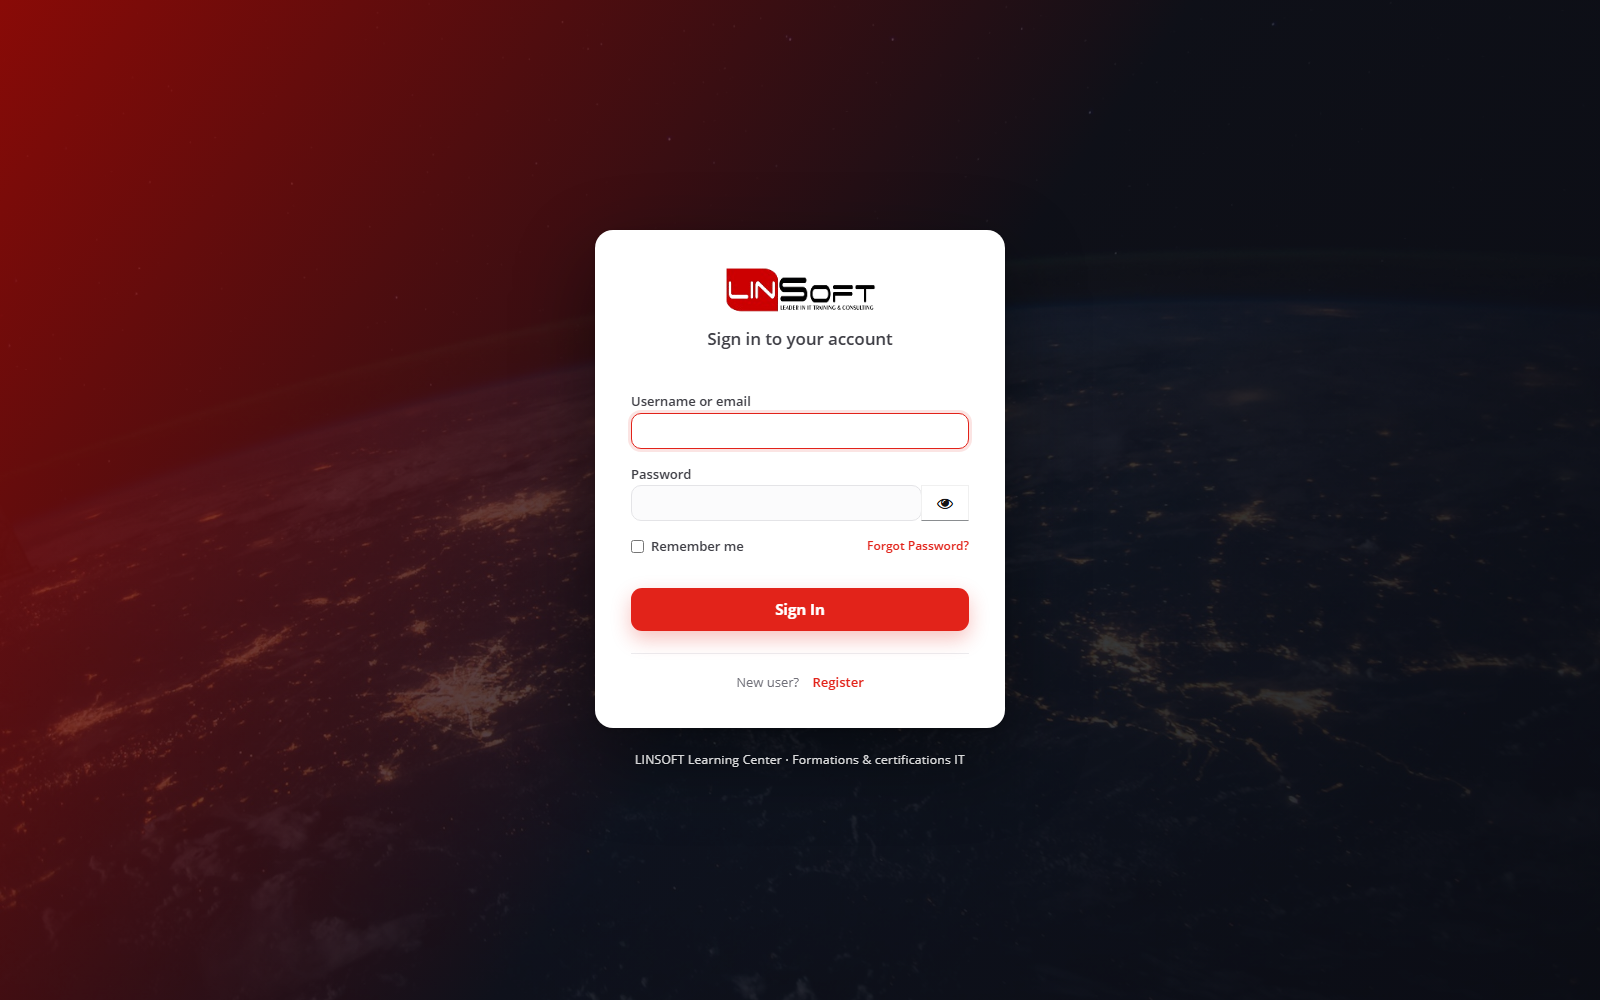
\includegraphics[width=0.92\textwidth]{captures/02-connexion-keycloak.png}
  \caption{Authentification déléguée à Keycloak, traversée automatiquement par les tests}
  \label{fig:e2e-login}
\end{figure}

Les scénarios couvrent l'authentification de chaque rôle, le rejet d'identifiants
invalides, et surtout le \textbf{cloisonnement} : un participant qui saisit l'adresse de
la console d'administration est détourné, un formateur ne peut pas atteindre la gestion des
certificats.

\begin{figure}[H]\centering
  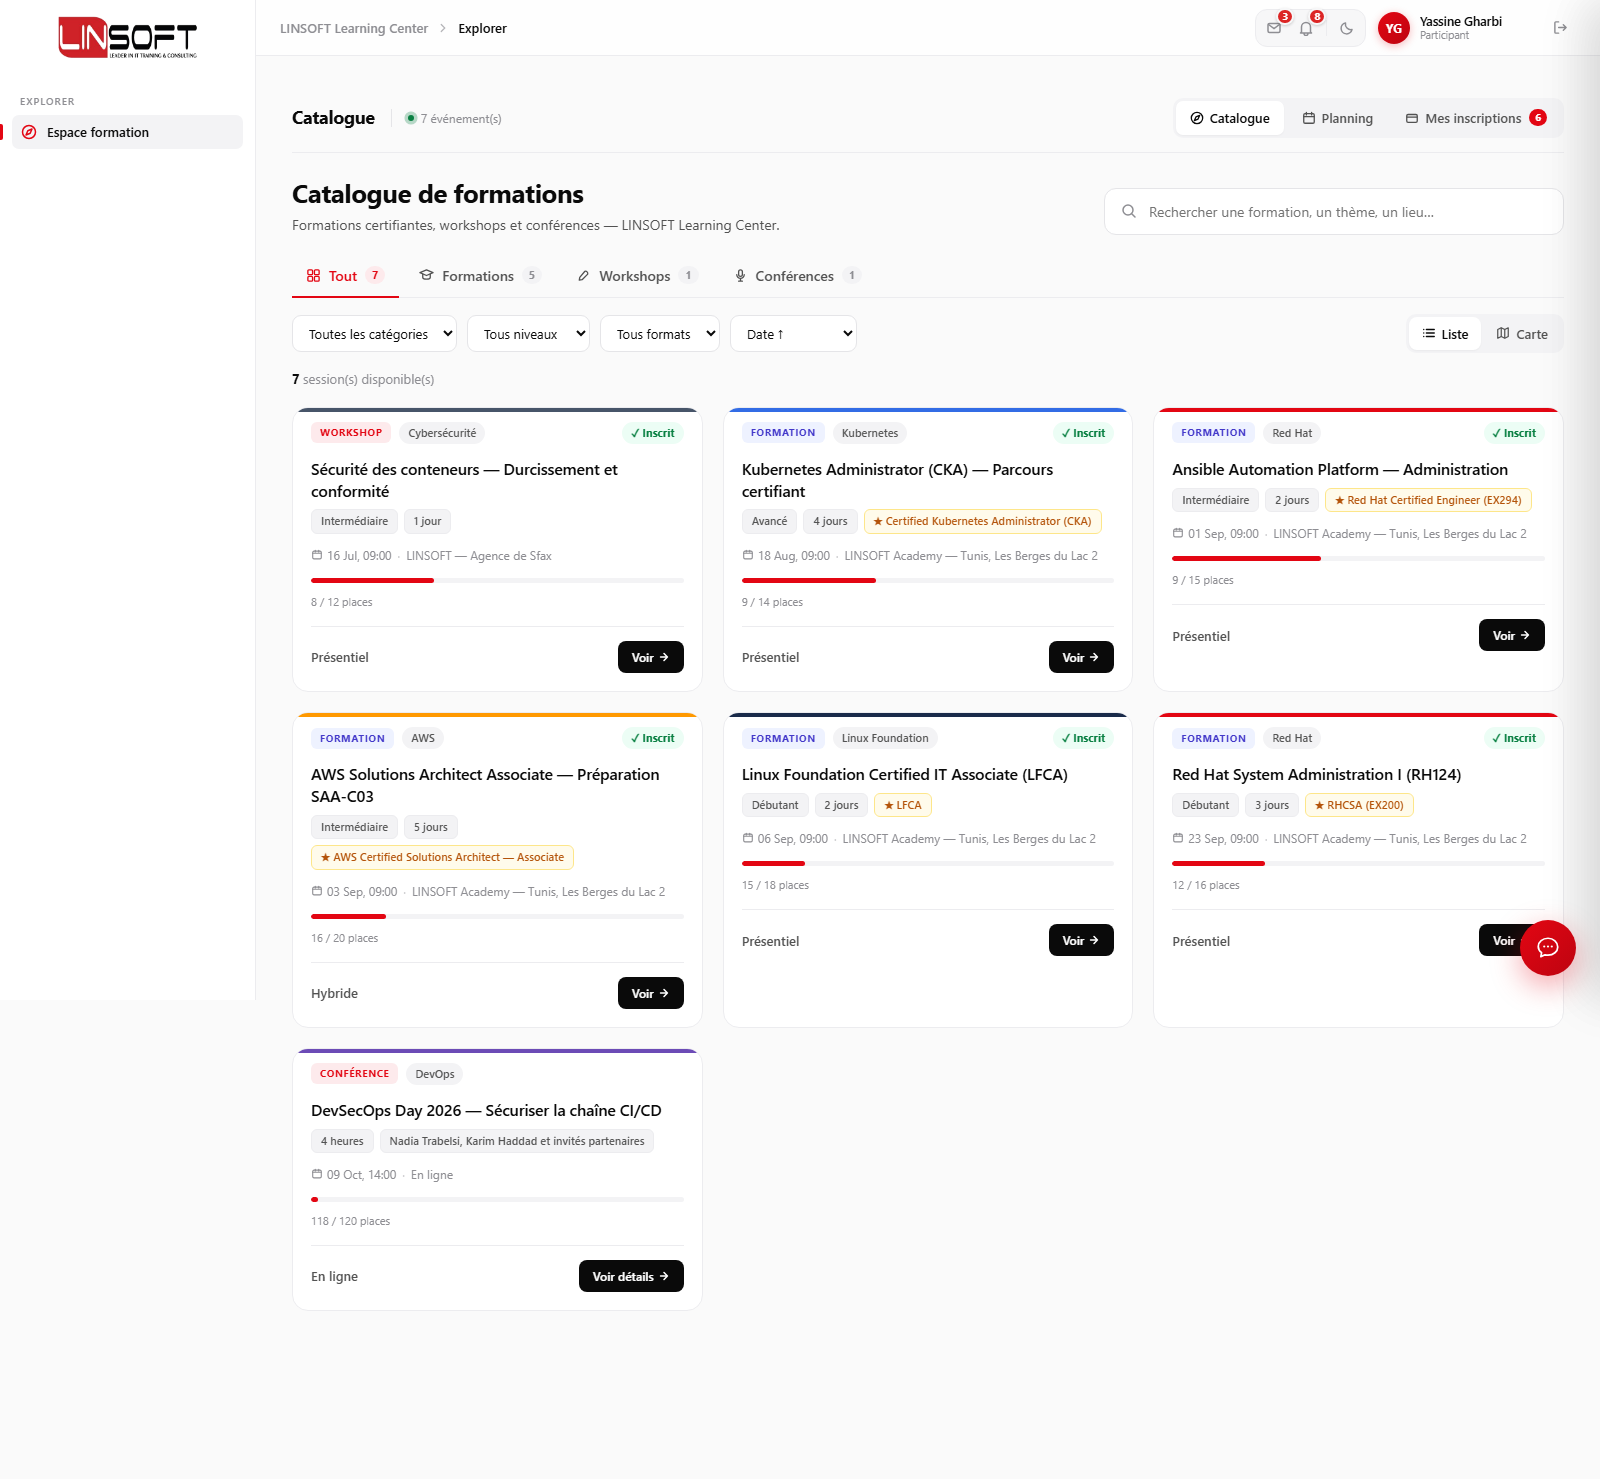
\includegraphics[width=0.92\textwidth]{captures/03-catalogue.png}
  \caption{Catalogue de formations — vue participant}
  \label{fig:devops-catalogue}
\end{figure}

%============================================================================
\section{Qualité du code et couverture}

\subsection{Outils d'analyse}
L'analyse statique (\textbf{Checkstyle} et \textbf{SpotBugs}) est regroupée dans un profil
Maven \texttt{quality}, activé à la demande et en intégration continue. Le jeu de règles
Checkstyle cible délibérément les défauts réels — comparaison de chaînes par
\texttt{==}, \texttt{equals} sans \texttt{hashCode}, blocs \texttt{catch} vides,
\texttt{switch} sans \texttt{default} — plutôt que la mise en forme : un jeu de règles trop
bavard finit systématiquement désactivé.

\subsection{Couverture mesurée}
\textbf{JaCoCo} produit des rapports HTML et XML par module. Le seuil est vérifié à chaque
\texttt{mvn verify} et fait échouer le build s'il n'est pas atteint.

\begin{table}[H]\centering\renewcommand{\arraystretch}{1.25}
\begin{tabular}{|p{5.5cm}|p{3cm}|}\hline
\rowcolor{gray!15}\textbf{Module} & \textbf{Couverture} \\ \hline
\texttt{feedback-service} & 78~\% \\ \hline
\texttt{notification-service} & 74~\% \\ \hline
\texttt{ticket-service} & 71~\% \\ \hline
\texttt{registration-service} & 61~\% \\ \hline
\texttt{event-service} & 53~\% \\ \hline
\texttt{ai-service} & 42~\% \\ \hline
\texttt{user-service} & 41~\% \\ \hline
\end{tabular}
\caption{Couverture des instructions, hors configuration, entités et DTO}\label{tab:couverture}
\end{table}

Le seuil a été relevé progressivement (0~\%, puis 25~\%, 30~\% et enfin 40~\%) au fur et à
mesure de l'écriture des tests. Ce choix est délibéré : un seuil ambitieux fixé d'emblée
aurait été inatteignable et n'aurait produit qu'une chose, sa propre désactivation. Le
seuil joue ainsi le rôle d'un \emph{cliquet anti-régression} plutôt que d'un objectif
décoratif. Son caractère réellement bloquant a été vérifié en le forçant temporairement à
90~\%, ce qui provoque bien l'échec du build.

%============================================================================
\section{Conteneurisation}

Chacun des onze composants dispose de son image. Les images backend reposent sur
\texttt{eclipse-temurin:17-jre-alpine} et appliquent \texttt{chgrp -R 0 /app}, condition
nécessaire sur OpenShift, qui exécute les conteneurs avec un identifiant utilisateur
aléatoire appartenant au groupe~0. Le frontend est construit en deux étapes
(\texttt{node:20-alpine} puis \texttt{nginx-unprivileged}) et s'exécute sans privilèges.

\subsection{Un défaut de conception corrigé}
Les images déclaraient déjà une directive \texttt{HEALTHCHECK} interrogeant
\texttt{/actuator/health}, \textbf{mais sept services sur dix n'embarquaient pas Actuator} :
la sonde recevait une réponse 404. Le fichier \texttt{docker-compose.yml} contournait le
problème par un \texttt{curl -s -o /dev/null || exit 1}, qui \emph{réussit même sur un 404
ou un 401}. Aucune vérification de santé du projet ne prouvait donc quoi que ce soit.
Actuator a été ajouté à tous les services via le POM parent, et les contournements
remplacés par de véritables vérifications.

%============================================================================
\section{Intégration et livraison continues}

\subsection{Architecture du pipeline}
La chaîne est décrite dans \texttt{.github/workflows/ci.yml} et s'exécute sur
\textbf{GitHub Actions} à chaque poussée et à chaque \emph{pull request}.

\begin{table}[H]\centering\renewcommand{\arraystretch}{1.25}
\begin{tabular}{|p{4cm}|p{9.5cm}|}\hline
\rowcolor{gray!15}\textbf{Étape} & \textbf{Contenu} \\ \hline
Tests backend & \texttt{mvn verify} : unitaires, API/sécurité, intégration, couverture \\ \hline
Analyse statique & Checkstyle et SpotBugs \\ \hline
Tests frontend & Vitest puis build de production \\ \hline
Images Docker & Onze images construites en parallèle \\ \hline
Analyse de sécurité & Trivy, vulnérabilités critiques et élevées \\ \hline
Publication & Registre GHCR, branche principale uniquement \\ \hline
Tests E2E & Plateforme complète démarrée, jeu de données semé, Playwright \\ \hline
\end{tabular}
\caption{Étapes de la chaîne d'intégration continue}\label{tab:pipeline}
\end{table}

\subsection{Choix : ne pas compiler dans les images}
Les fichiers \texttt{Dockerfile} du backend copient une archive JAR déjà construite plutôt
que de la compiler. Une construction multi-étapes par service recompilerait dix fois le même
réacteur Maven, pour un résultat identique. Le réacteur est donc construit \textbf{une
seule fois}, les archives circulent en artefact entre les étapes, et chaque image est
assemblée à partir du binaire validé : l'artefact testé et l'artefact publié sont ainsi le
même objet.

\subsection{Garde-fou contre les faux positifs}
Une étape vérifie explicitement qu'\textbf{aucun test d'intégration n'a été ignoré} alors
que Docker était disponible. Sans ce contrôle, un environnement dépourvu de Docker
produirait un pipeline vert trompeur, puisque les tests Testcontainers s'ignorent
automatiquement en l'absence de démon.

\subsection{Deux défauts révélés par les premières exécutions}
Aucun des deux n'était détectable en local, ce qui illustre précisément l'apport d'une
chaîne d'intégration continue.

\begin{enumerate}
  \item \textbf{Référence d'action non résolue.} Les onze tâches de construction d'images
        échouaient à l'étape « Set up job », c'est-à-dire \emph{avant} leur première
        instruction. Les étiquettes du dépôt \texttt{trivy-action} sont préfixées par
        \texttt{v} : la référence \texttt{@0.28.0} n'existait pas. GitHub Actions résout les
        actions avant de les exécuter, d'où un échec sans aucune trace dans les étapes.
  \item \textbf{Nom d'image refusé par le registre.} Une fois ce point corrigé, la
        construction, l'analyse Trivy et l'authentification réussissaient, mais la
        publication échouait — symptôme trompeur. Le compte GitHub s'écrit
        \texttt{Medamine009}, avec une majuscule, alors que GHCR n'accepte que des noms
        d'image en minuscules. Le nom est désormais normalisé avant usage.
\end{enumerate}

%============================================================================
\section{Supervision et observabilité}

\subsection{Points de mesure}
Tous les services exposent, via Actuator et Micrometer, un agrégat de santé, des sondes
distinctes de \emph{liveness} et de \emph{readiness}, ainsi que leurs métriques au format
Prometheus. L'exposition est volontairement restreinte aux points réellement utilisés :
\texttt{env}, \texttt{beans} et \texttt{heapdump} restent fermés.

\subsection{Collecte et visualisation}
Prometheus interroge les dix services toutes les quinze secondes ; Grafana en propose la
lecture. L'ensemble est placé derrière un profil Docker Compose afin de ne pas alourdir le
démarrage courant de la plateforme.

\begin{figure}[H]\centering
  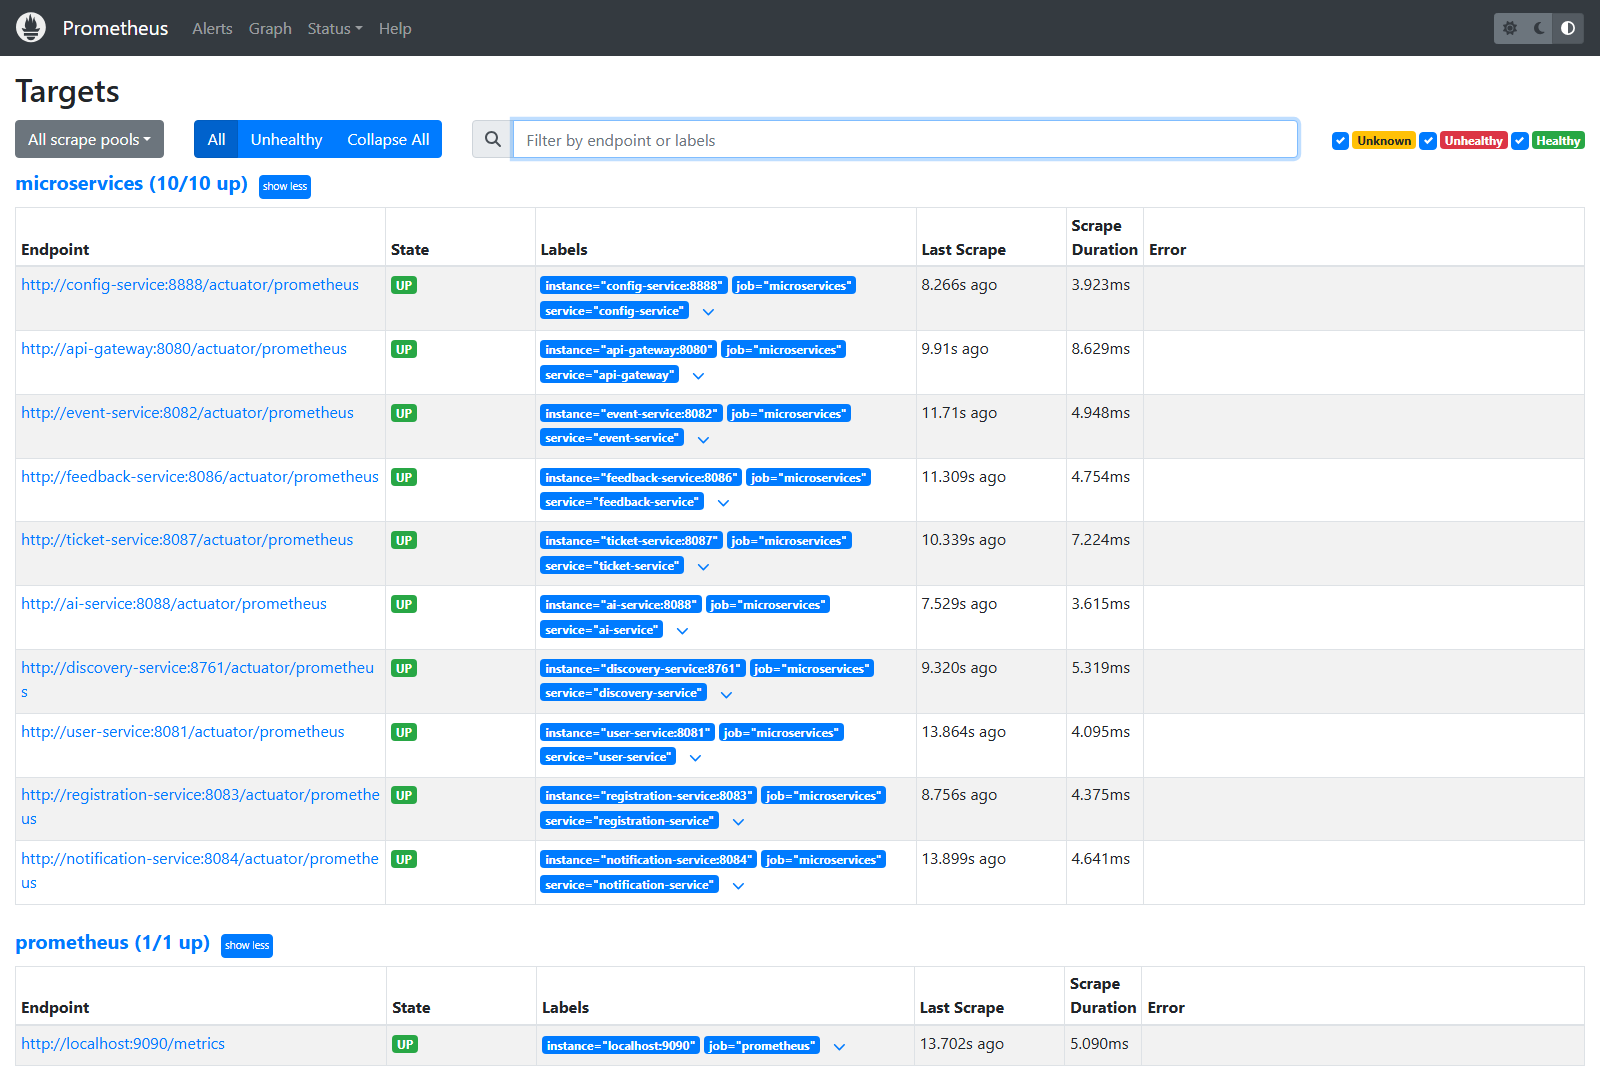
\includegraphics[width=0.92\textwidth]{captures/08-prometheus-cibles.png}
  \caption{Cibles Prometheus : les dix microservices interrogés avec succès}
  \label{fig:prometheus}
\end{figure}

\begin{figure}[H]\centering
  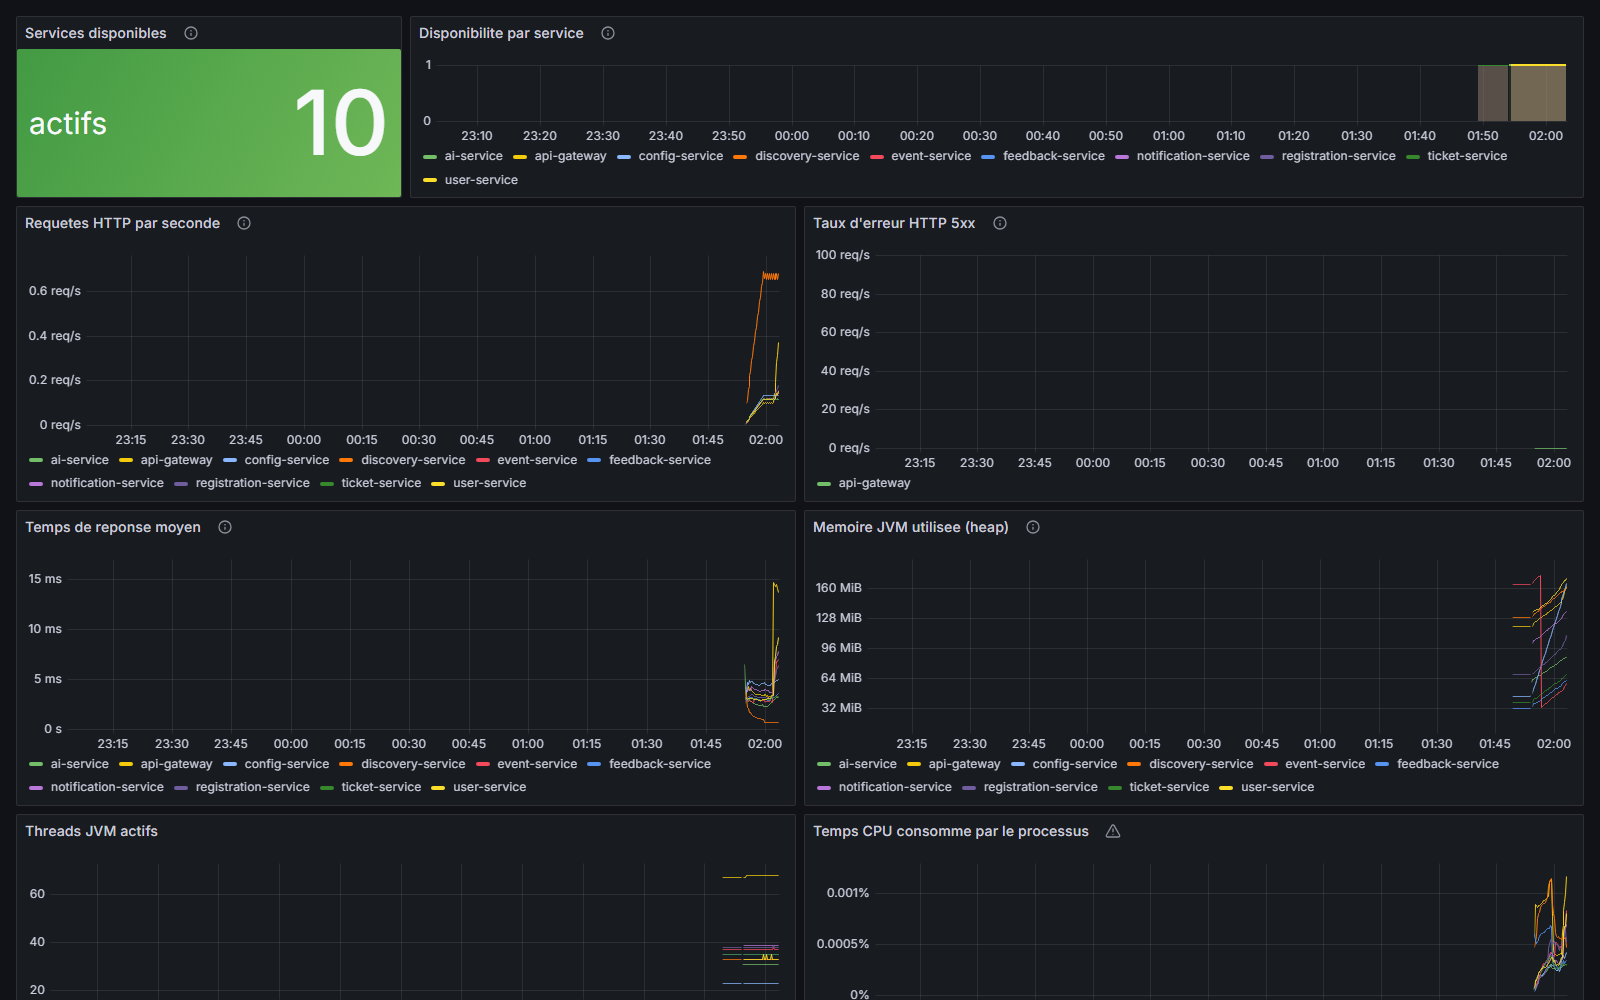
\includegraphics[width=\textwidth]{captures/09-grafana-plateforme.png}
  \caption{Tableau de bord Grafana : disponibilité, charge, temps de réponse et mémoire}
  \label{fig:grafana}
\end{figure}

Chaque série porte une étiquette \texttt{application} apposée par Micrometer ; sans elle,
les séries des dix services seraient indistinguables.

\begin{figure}[H]\centering
  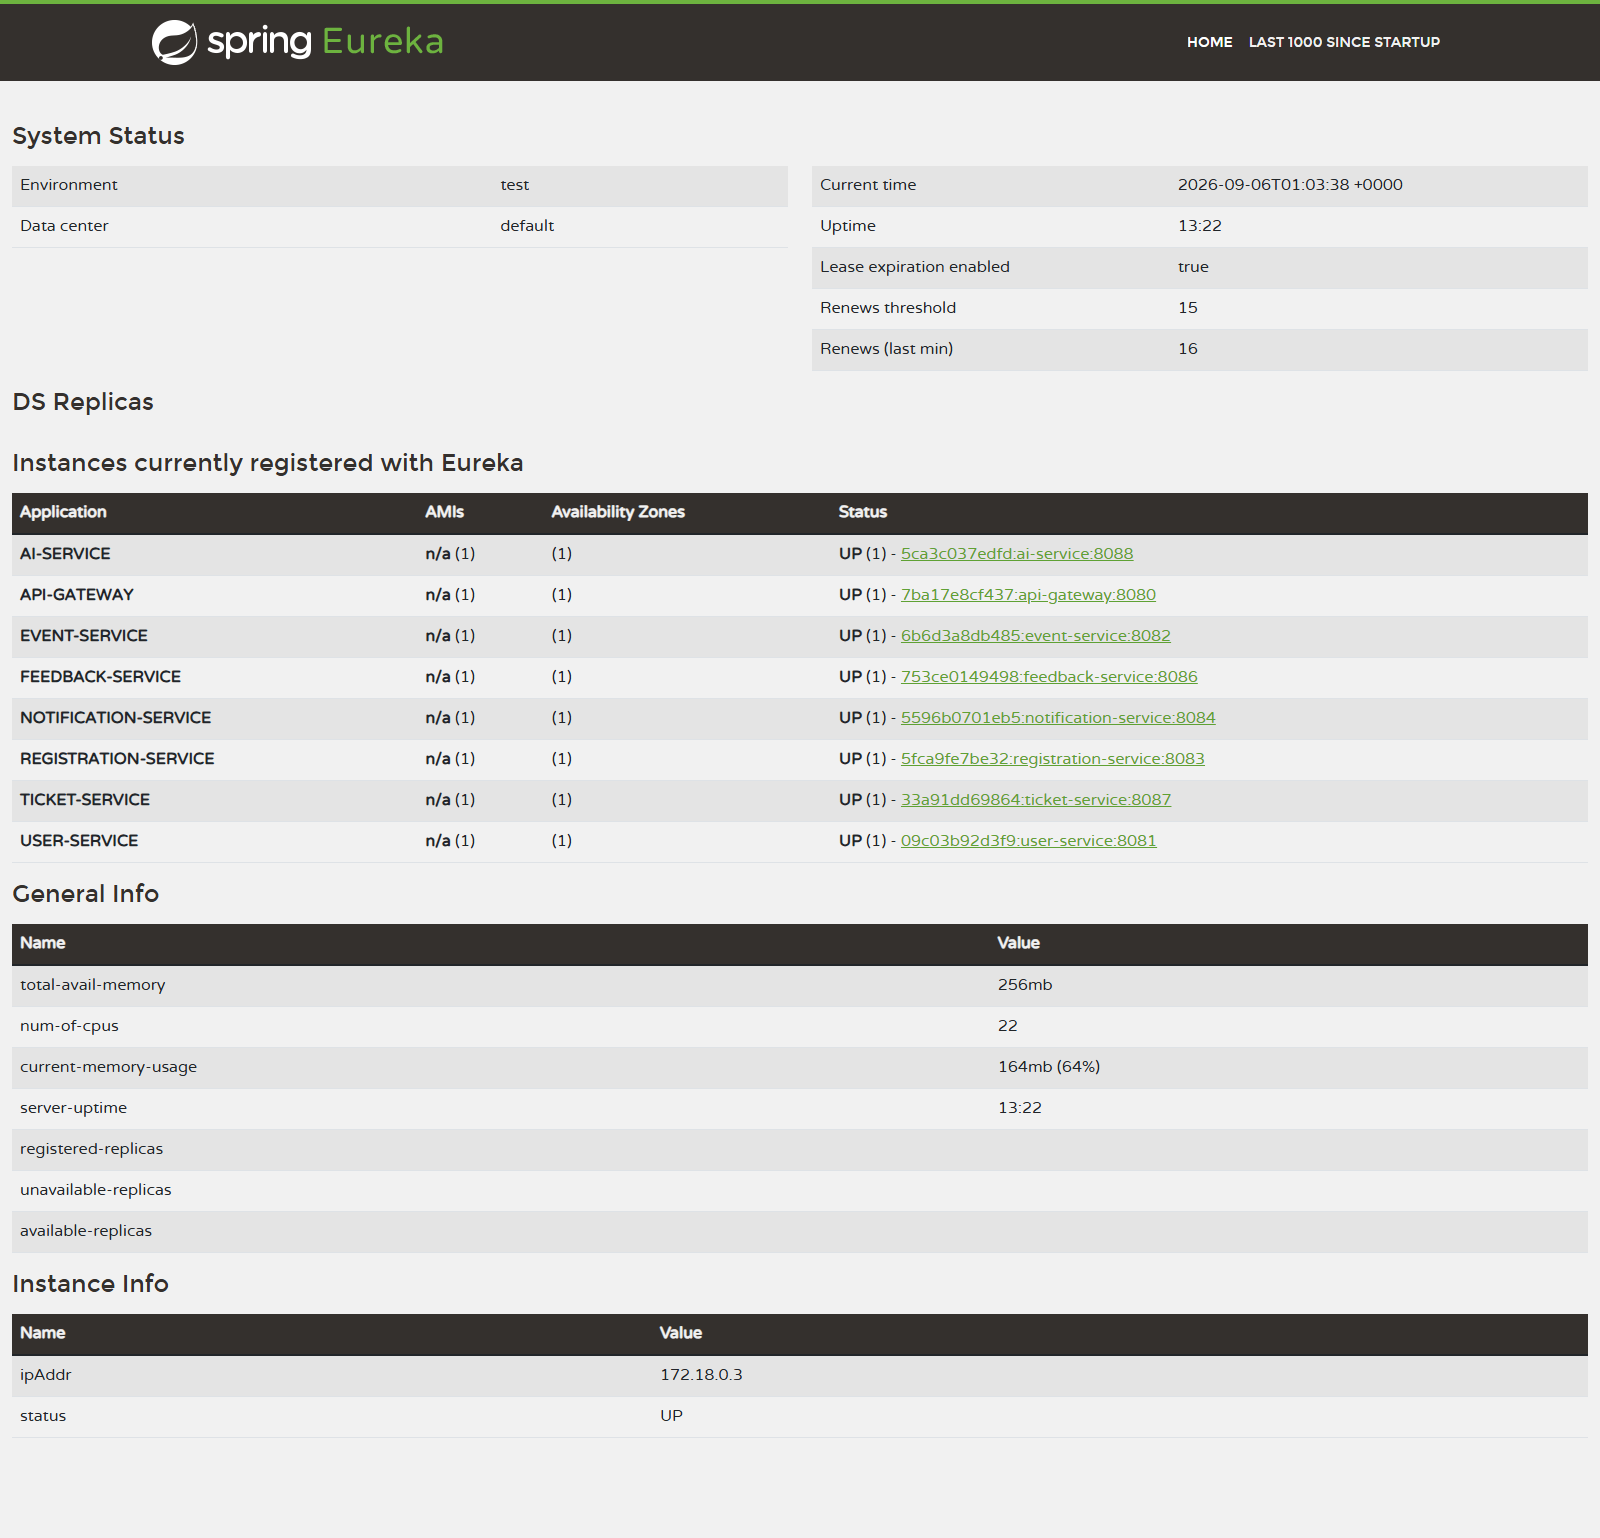
\includegraphics[width=0.92\textwidth]{captures/11-eureka.png}
  \caption{Registre Eureka : services enregistrés et découverte dynamique}
  \label{fig:eureka}
\end{figure}

\begin{figure}[H]\centering
  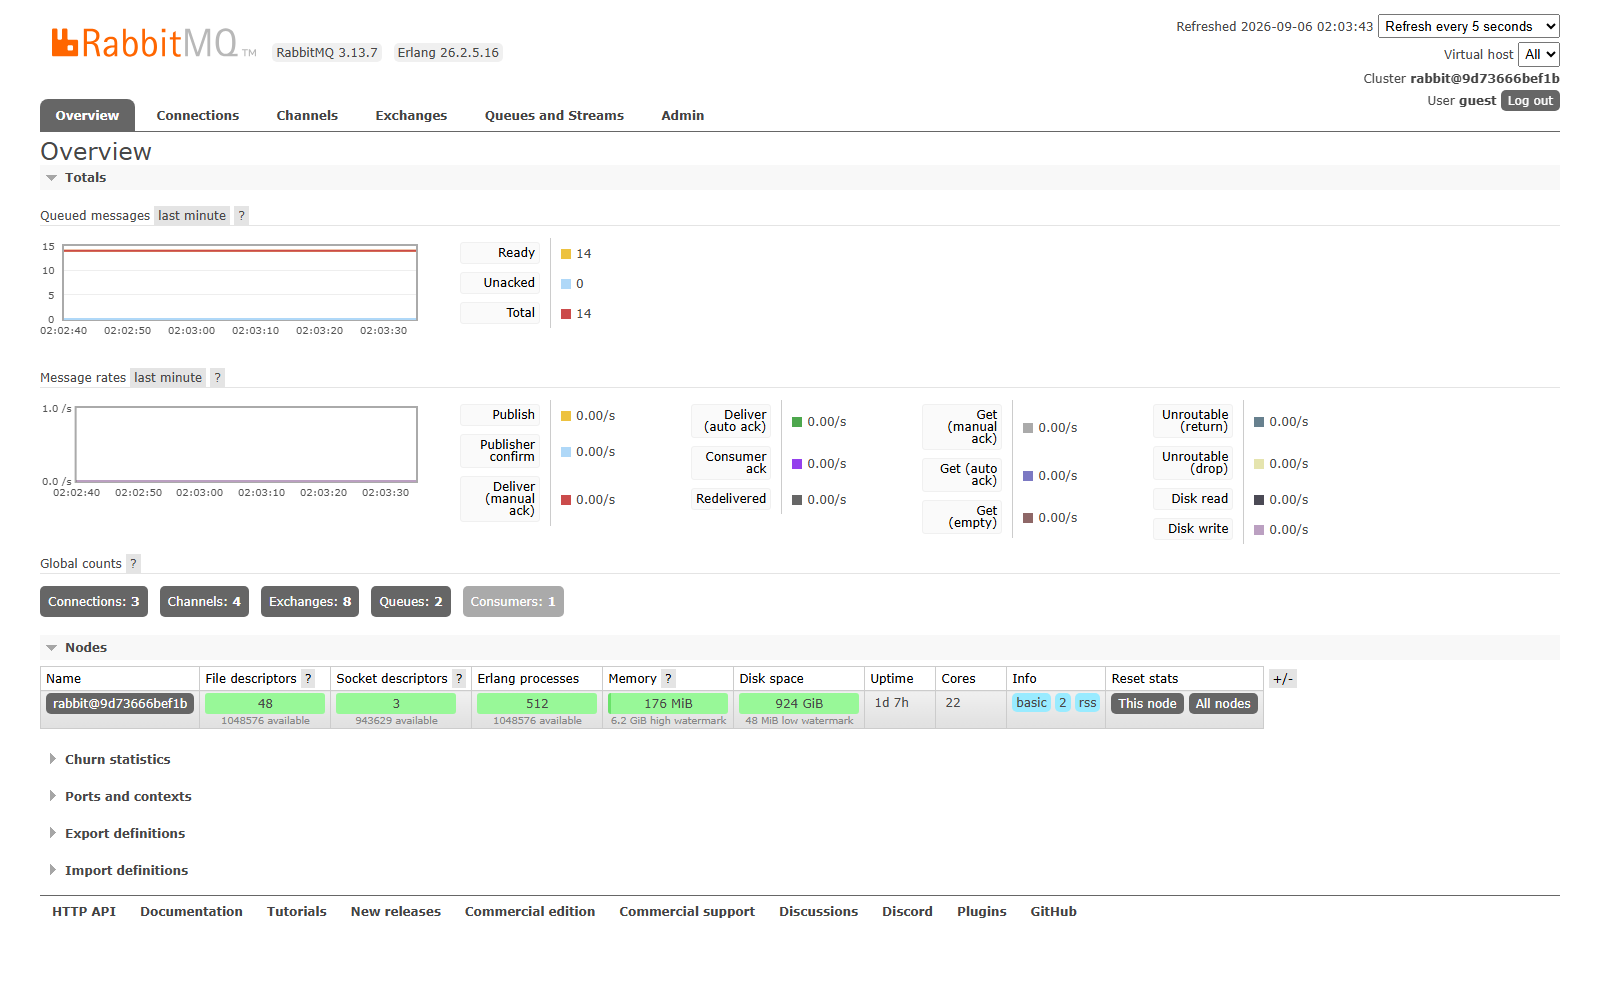
\includegraphics[width=0.92\textwidth]{captures/12-rabbitmq.png}
  \caption{Console RabbitMQ : file de notifications et débit des messages}
  \label{fig:rabbitmq}
\end{figure}

%============================================================================
\section{Sécurité de la chaîne}

\begin{itemize}
  \item \textbf{Analyse des images} : Trivy inspecte chaque image et remonte les
        vulnérabilités critiques et élevées dans l'onglet \emph{Security} du dépôt.
  \item \textbf{Aucun secret versionné} : la publication utilise le jeton fourni par la
        plateforme. Le fichier \texttt{.env} est exclu du dépôt et accompagné d'un modèle
        \texttt{.env.example}.
  \item \textbf{Secrets de déploiement} : un script \texttt{create-secrets.sh} génère des
        mots de passe aléatoires via \texttt{oc create secret}, de sorte qu'aucune valeur
        réelle ne transite par Git.
\end{itemize}

%============================================================================
\section{Illustrations du parcours fonctionnel}

Les captures suivantes montrent le résultat obtenu sur les fonctionnalités les plus
structurantes, avec le jeu de données de démonstration.

\begin{figure}[H]\centering
  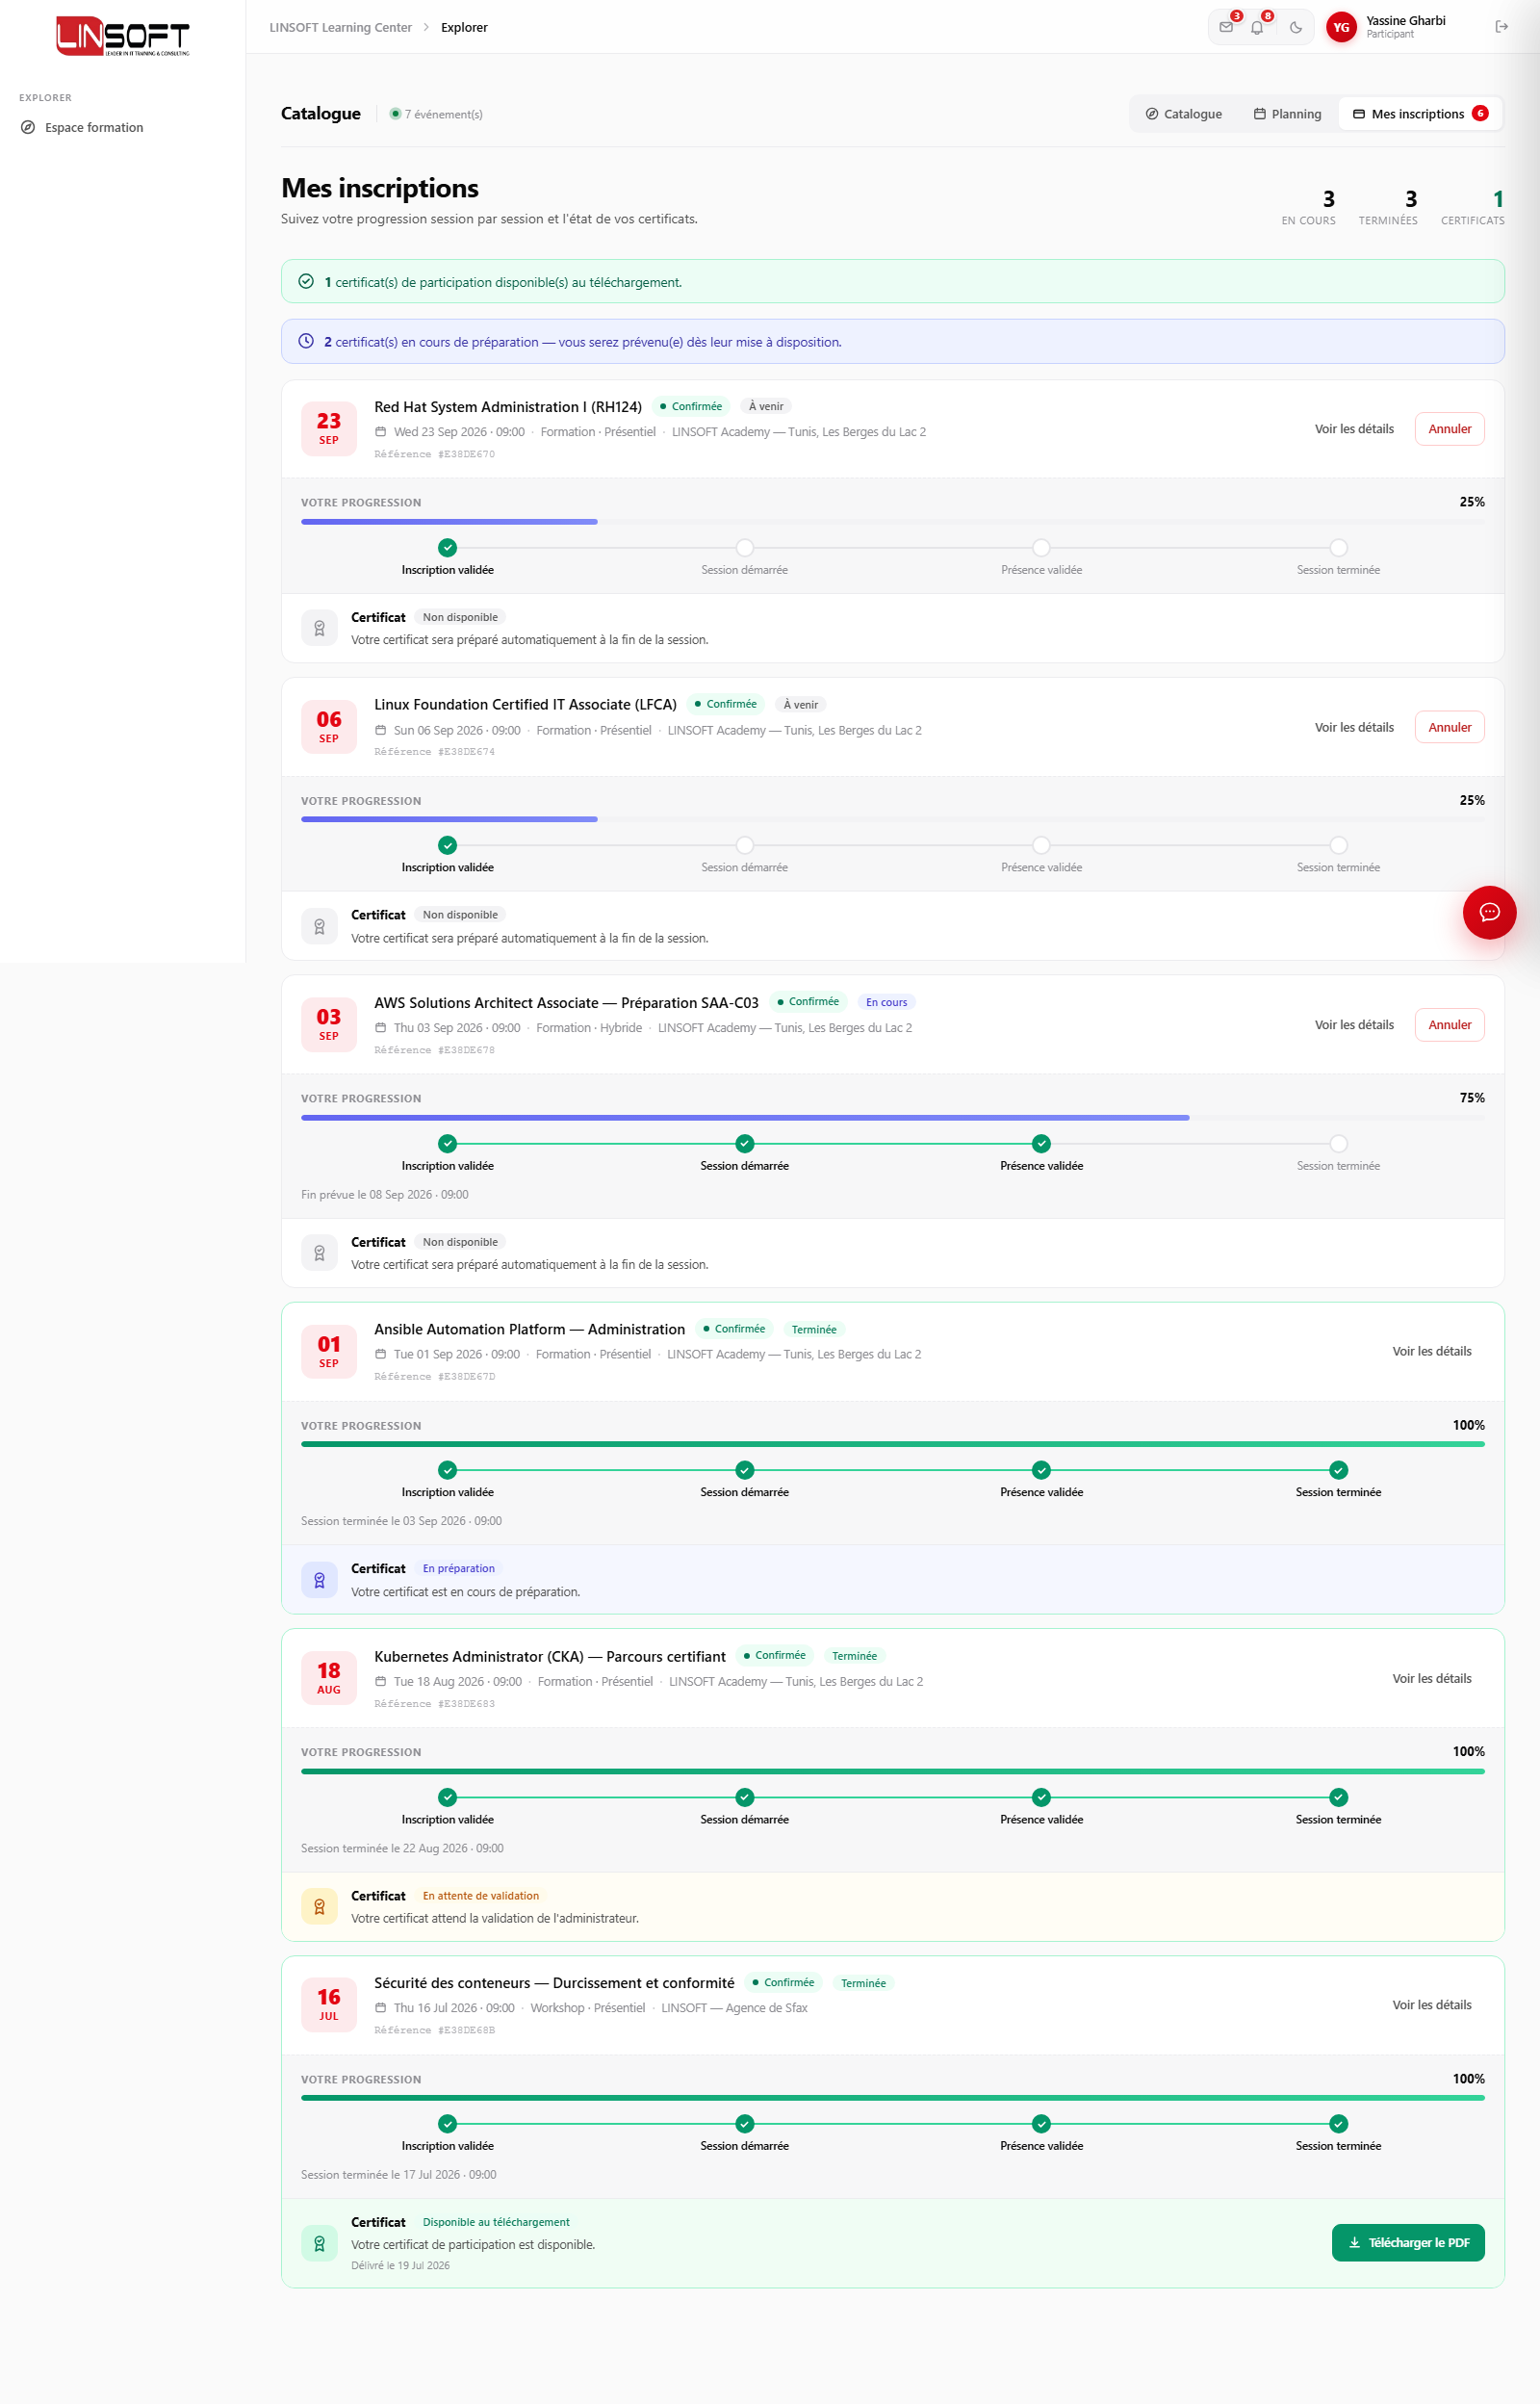
\includegraphics[width=0.85\textwidth]{captures/04-suivi-certificats.png}
  \caption{Suivi de participation : progression par jalons et cycle de vie du certificat}
  \label{fig:suivi}
\end{figure}

Cette vue rassemble les cinq états du parcours : session à venir (certificat non
disponible), session en cours avec progression intermédiaire, puis session terminée avec un
certificat successivement \emph{en préparation}, \emph{en attente de validation} et enfin
\emph{disponible au téléchargement}.

\begin{figure}[H]\centering
  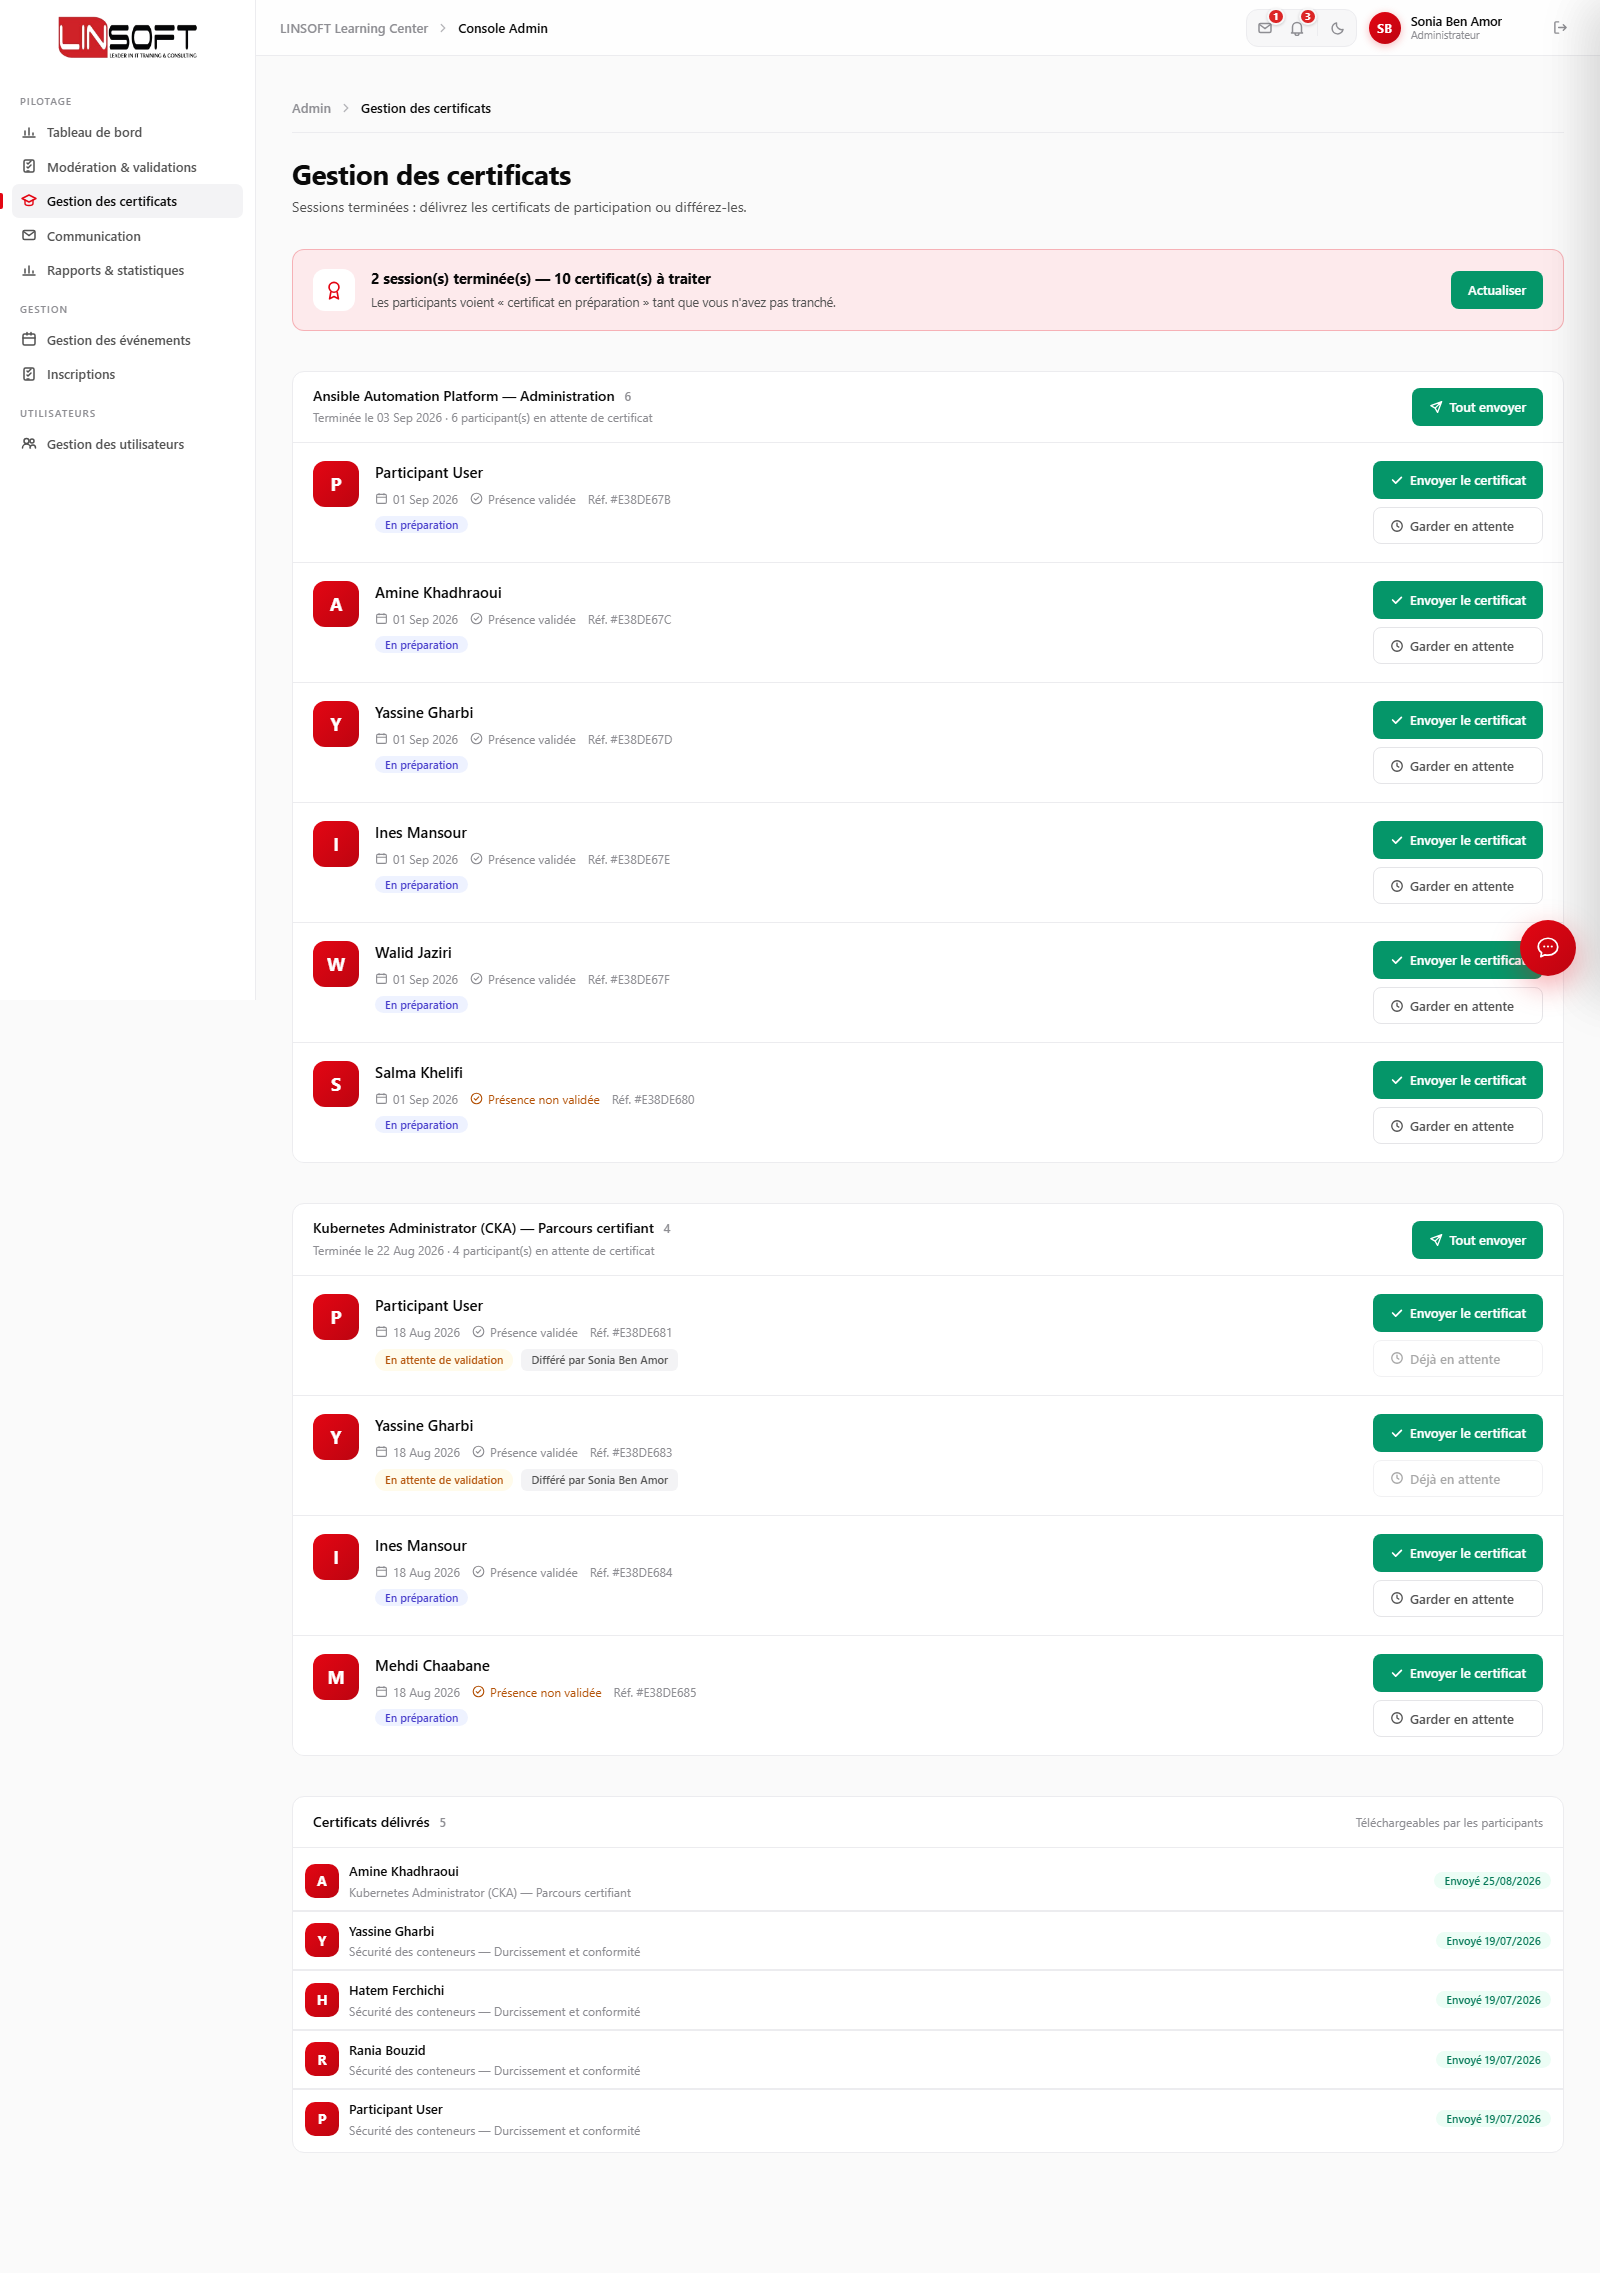
\includegraphics[width=0.85\textwidth]{captures/06-gestion-certificats.png}
  \caption{Console d'administration : file des certificats à délivrer, groupée par session}
  \label{fig:certificats-admin}
\end{figure}

\begin{figure}[H]\centering
  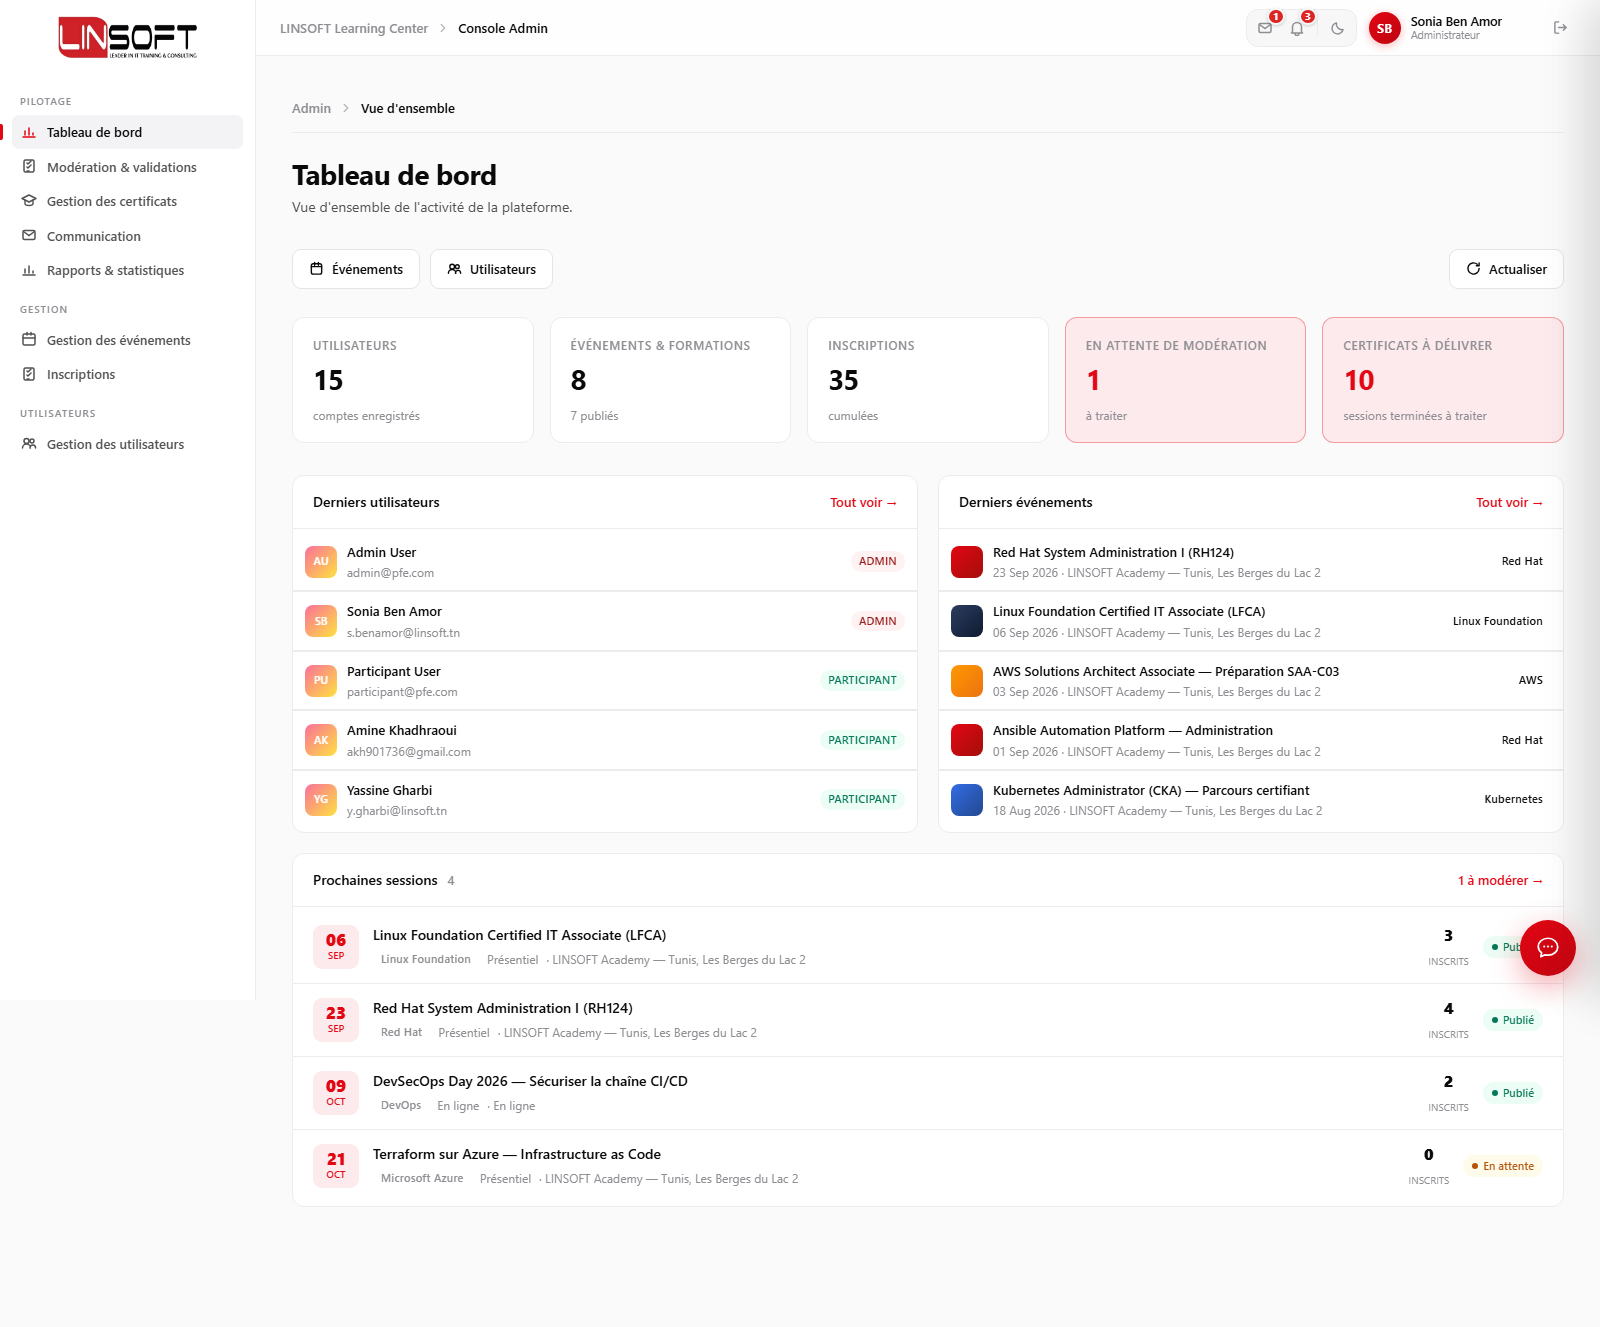
\includegraphics[width=0.92\textwidth]{captures/05-admin-dashboard.png}
  \caption{Tableau de bord administrateur et indicateurs de la plateforme}
  \label{fig:admin}
\end{figure}

\begin{figure}[H]\centering
  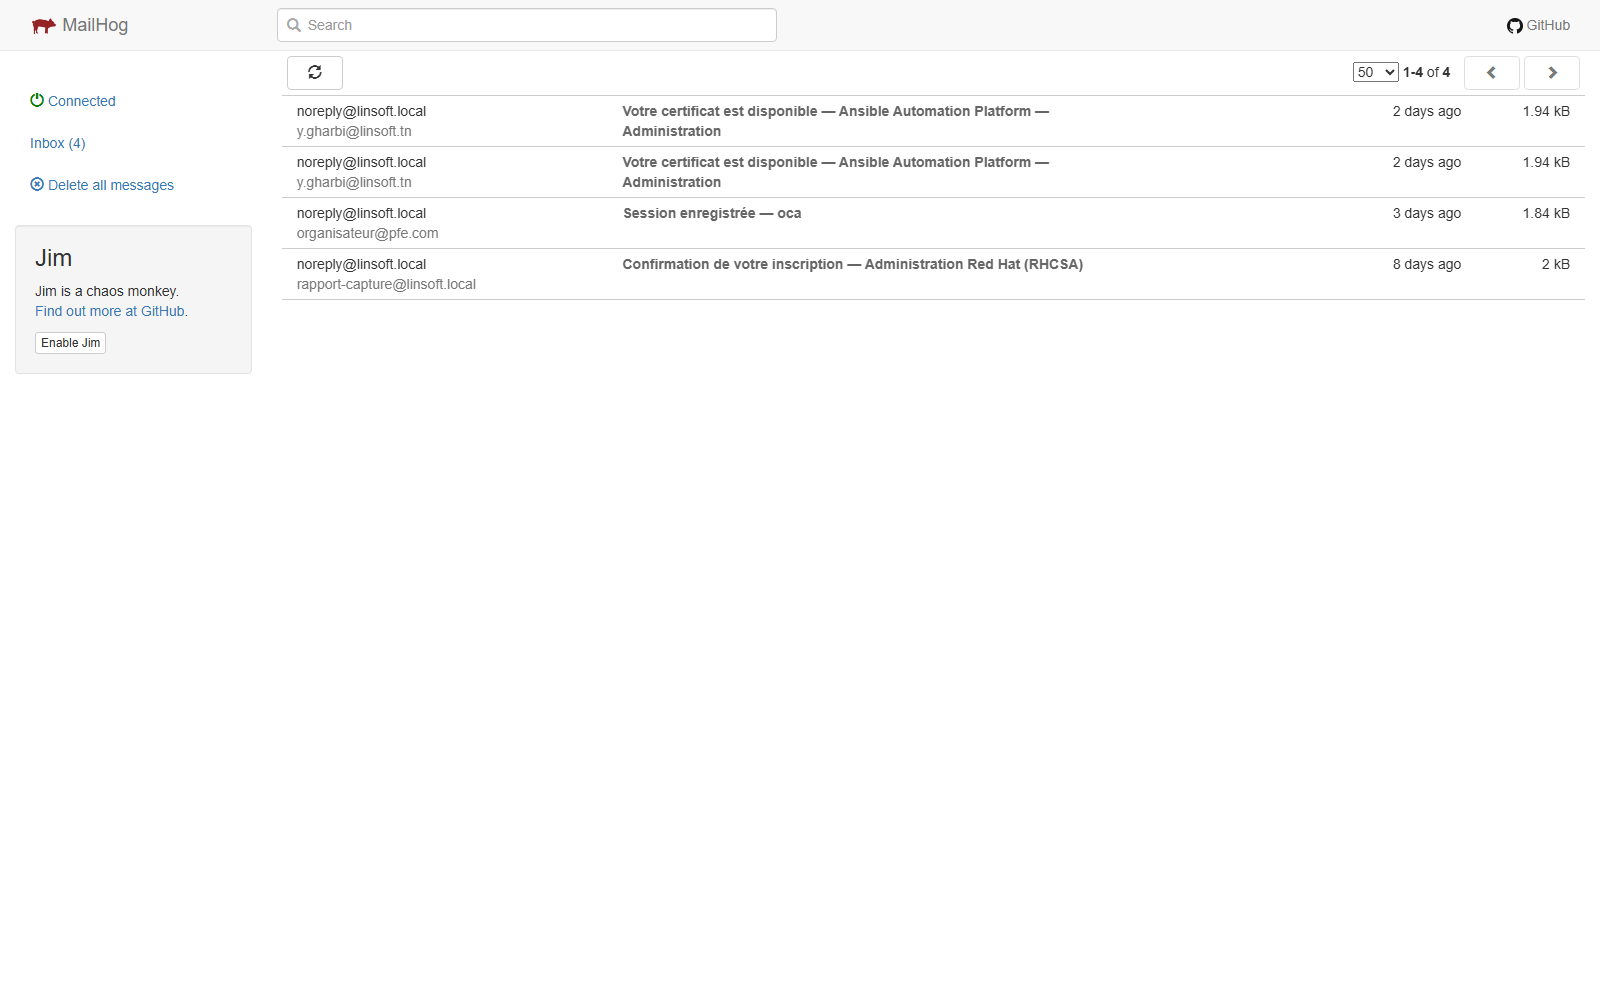
\includegraphics[width=0.92\textwidth]{captures/10-mailhog.png}
  \caption{Courriels émis par la plateforme, interceptés par MailHog en environnement de test}
  \label{fig:mailhog}
\end{figure}

%============================================================================
\section*{Conclusion}
La démarche présentée dans ce chapitre a fait passer le projet de dix-huit tests sans mesure
de couverture à près de trois cents tests répartis sur quatre niveaux, adossés à une chaîne
d'intégration continue de dix-sept tâches et à un dispositif de supervision opérationnel.
Au-delà des chiffres, cette démarche a démontré sa valeur en révélant des défauts réels et
invisibles autrement : des vérifications de santé qui ne vérifiaient rien, une référence
d'action inexistante, un nom d'image refusé par le registre, et une référence de dossier
identique pour toute une promotion de participants.

%  Les captures référencées se trouvent dans rapport-pfe/captures/
%############################################################################
\chapter{Tests, qualité et démarche DevOps}

\section*{Introduction}
Une plateforme composée de dix microservices ne se valide pas en la parcourant à la main :
le nombre de combinaisons de rôles, d'états et de services rend la vérification manuelle
à la fois incomplète et non reproductible. Ce chapitre présente la stratégie de test mise
en place, les outils de mesure de la qualité, la chaîne d'intégration continue et le
dispositif de supervision. Chaque choix y est justifié par le défaut qu'il permet de
détecter, et les résultats présentés sont ceux réellement obtenus sur la plateforme.

%============================================================================
\section{Stratégie de test}

\subsection{Pyramide de test retenue}
Quatre niveaux de test se répondent, chacun apportant une garantie que les autres ne
peuvent pas fournir.

\begin{table}[H]\centering\renewcommand{\arraystretch}{1.3}
\begin{tabular}{|p{3.2cm}|p{5cm}|p{6cm}|}\hline
\rowcolor{gray!15}\textbf{Niveau} & \textbf{Outils} & \textbf{Question à laquelle il répond} \\ \hline
Unitaire & JUnit 5, Mockito & La règle métier est-elle juste ? \\ \hline
API / Sécurité & MockMvc, spring-security-test & L'API applique-t-elle réellement les droits ? \\ \hline
Intégration & Testcontainers (MongoDB) & Le code dialogue-t-il correctement avec une base réelle ? \\ \hline
Bout en bout & Playwright, Chromium & Le parcours utilisateur fonctionne-t-il entièrement ? \\ \hline
\end{tabular}
\caption{Niveaux de test et rôle de chacun}\label{tab:pyramide}
\end{table}

\subsection{Séparation des tests rapides et des tests d'infrastructure}
La convention de nommage pilote l'exécution, configurée une seule fois dans le POM parent :
les classes \texttt{*Test} sont exécutées par Surefire pendant la phase \texttt{test}, les
classes \texttt{*IT} par Failsafe pendant la phase \texttt{verify}. Le développeur dispose
ainsi d'une boucle de retour courte (\texttt{mvn test}, sans infrastructure), tandis que
l'intégration continue exécute la chaîne complète (\texttt{mvn verify}).

\subsection{Répartition obtenue}
\begin{table}[H]\centering\renewcommand{\arraystretch}{1.25}
\begin{tabular}{|p{5cm}|p{2.6cm}|p{2.6cm}|}\hline
\rowcolor{gray!15}\textbf{Périmètre} & \textbf{Avant} & \textbf{Après} \\ \hline
Tests backend & 18 & \textbf{195} \\ \hline
Tests frontend & 53 (dont 1 en échec) & \textbf{82} \\ \hline
Tests de bout en bout & 0 & \textbf{14} \\ \hline
Mesure de couverture & aucune & JaCoCo, seuil à 40~\% \\ \hline
\end{tabular}
\caption{Évolution de la couverture de test du projet}\label{tab:devops-tests}
\end{table}

\subsection{Exemples de règles protégées}
Les tests ne visent pas le taux de couverture pour lui-même, mais les règles dont la
défaillance produirait un défaut visible :

\begin{itemize}
  \item l'annulation d'une \emph{demande en attente} ne doit pas libérer une place qui
        n'avait jamais été réservée, sous peine de créer des places fantômes ;
  \item un second scan du même QR code renvoie \texttt{ALREADY} plutôt que d'autoriser
        une seconde entrée ;
  \item l'envoi d'un certificat est idempotent : un double clic de l'administrateur ne
        déclenche pas un second courriel ;
  \item un message RabbitMQ malformé ne doit pas remonter en exception, sans quoi le
        courtier le redistribuerait en boucle et bloquerait la file pour tous les
        destinataires ;
  \item une session dont la durée est illisible n'est jamais clôturée par anticipation :
        le calcul retombe sur une journée type.
\end{itemize}

\subsection{Tests de sécurité}
Les tests de contrôleur chargent la \textbf{configuration de sécurité de production}
(\texttt{@Import(SecurityConfig.class)}) et non une sécurité désactivée : ce qui est
vérifié est donc bien ce qui s'appliquera en exploitation. Des jetons JWT sont simulés
avec les rôles Keycloak correspondants.

\begin{table}[H]\centering\renewcommand{\arraystretch}{1.25}
\begin{tabular}{|p{8.5cm}|p{4cm}|}\hline
\rowcolor{gray!15}\textbf{Scénario} & \textbf{Réponse attendue} \\ \hline
Appel sans jeton & \texttt{401} \\ \hline
Vérification publique d'un billet & \texttt{200} sans authentification \\ \hline
File des certificats — participant ou formateur & \texttt{403} \\ \hline
Certificat personnel, déjà envoyé & \texttt{200} + \texttt{application/pdf} \\ \hline
Certificat personnel, en préparation & \texttt{409} \\ \hline
Certificat d'un autre participant & \texttt{403} \\ \hline
\end{tabular}
\caption{Contrôle d'accès vérifié par les tests}\label{tab:securite}
\end{table}

La distinction entre \texttt{403} et \texttt{409} est délibérée : elle permet à l'interface
d'afficher « vous n'avez pas le droit » ou « votre certificat n'est pas encore délivré »,
deux messages très différents pour l'utilisateur.

\subsection{Tests d'intégration avec Testcontainers}
Les tests d'intégration démarrent un conteneur \textbf{MongoDB} éphémère, créé et détruit
par le test lui-même : aucune base locale n'est requise, et le résultat ne dépend pas du
poste du développeur. Ils valident ce que des simulacres ne peuvent pas prouver — les
requêtes réellement exécutées, et la persistance complète de l'entité, horodatages compris.

%============================================================================
\section{Tests de bout en bout}

Quatorze scénarios sont exécutés dans un navigateur Chromium réel, contre la plateforme
entièrement démarrée. C'est le seul niveau capable de prouver que la chaîne complète — clic,
redirection Keycloak, jeton, passerelle, microservice, rendu Angular — fonctionne ensemble.

\begin{figure}[H]\centering
  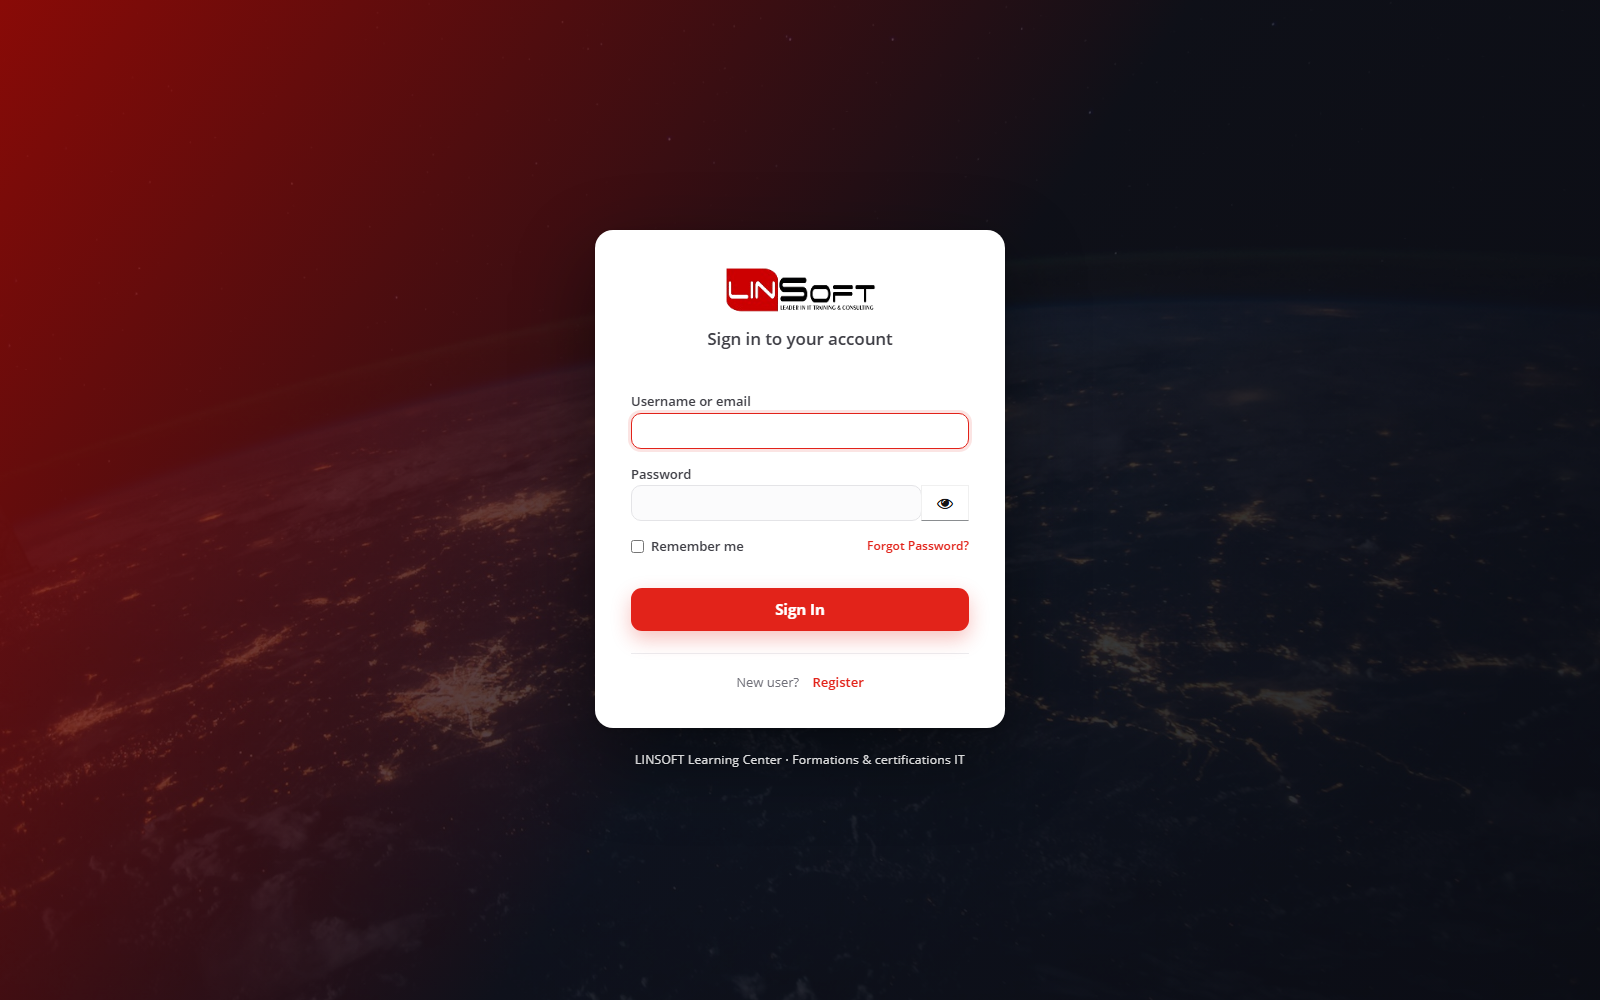
\includegraphics[width=0.92\textwidth]{captures/02-connexion-keycloak.png}
  \caption{Authentification déléguée à Keycloak, traversée automatiquement par les tests}
  \label{fig:e2e-login}
\end{figure}

Les scénarios couvrent l'authentification de chaque rôle, le rejet d'identifiants
invalides, et surtout le \textbf{cloisonnement} : un participant qui saisit l'adresse de
la console d'administration est détourné, un formateur ne peut pas atteindre la gestion des
certificats.

\begin{figure}[H]\centering
  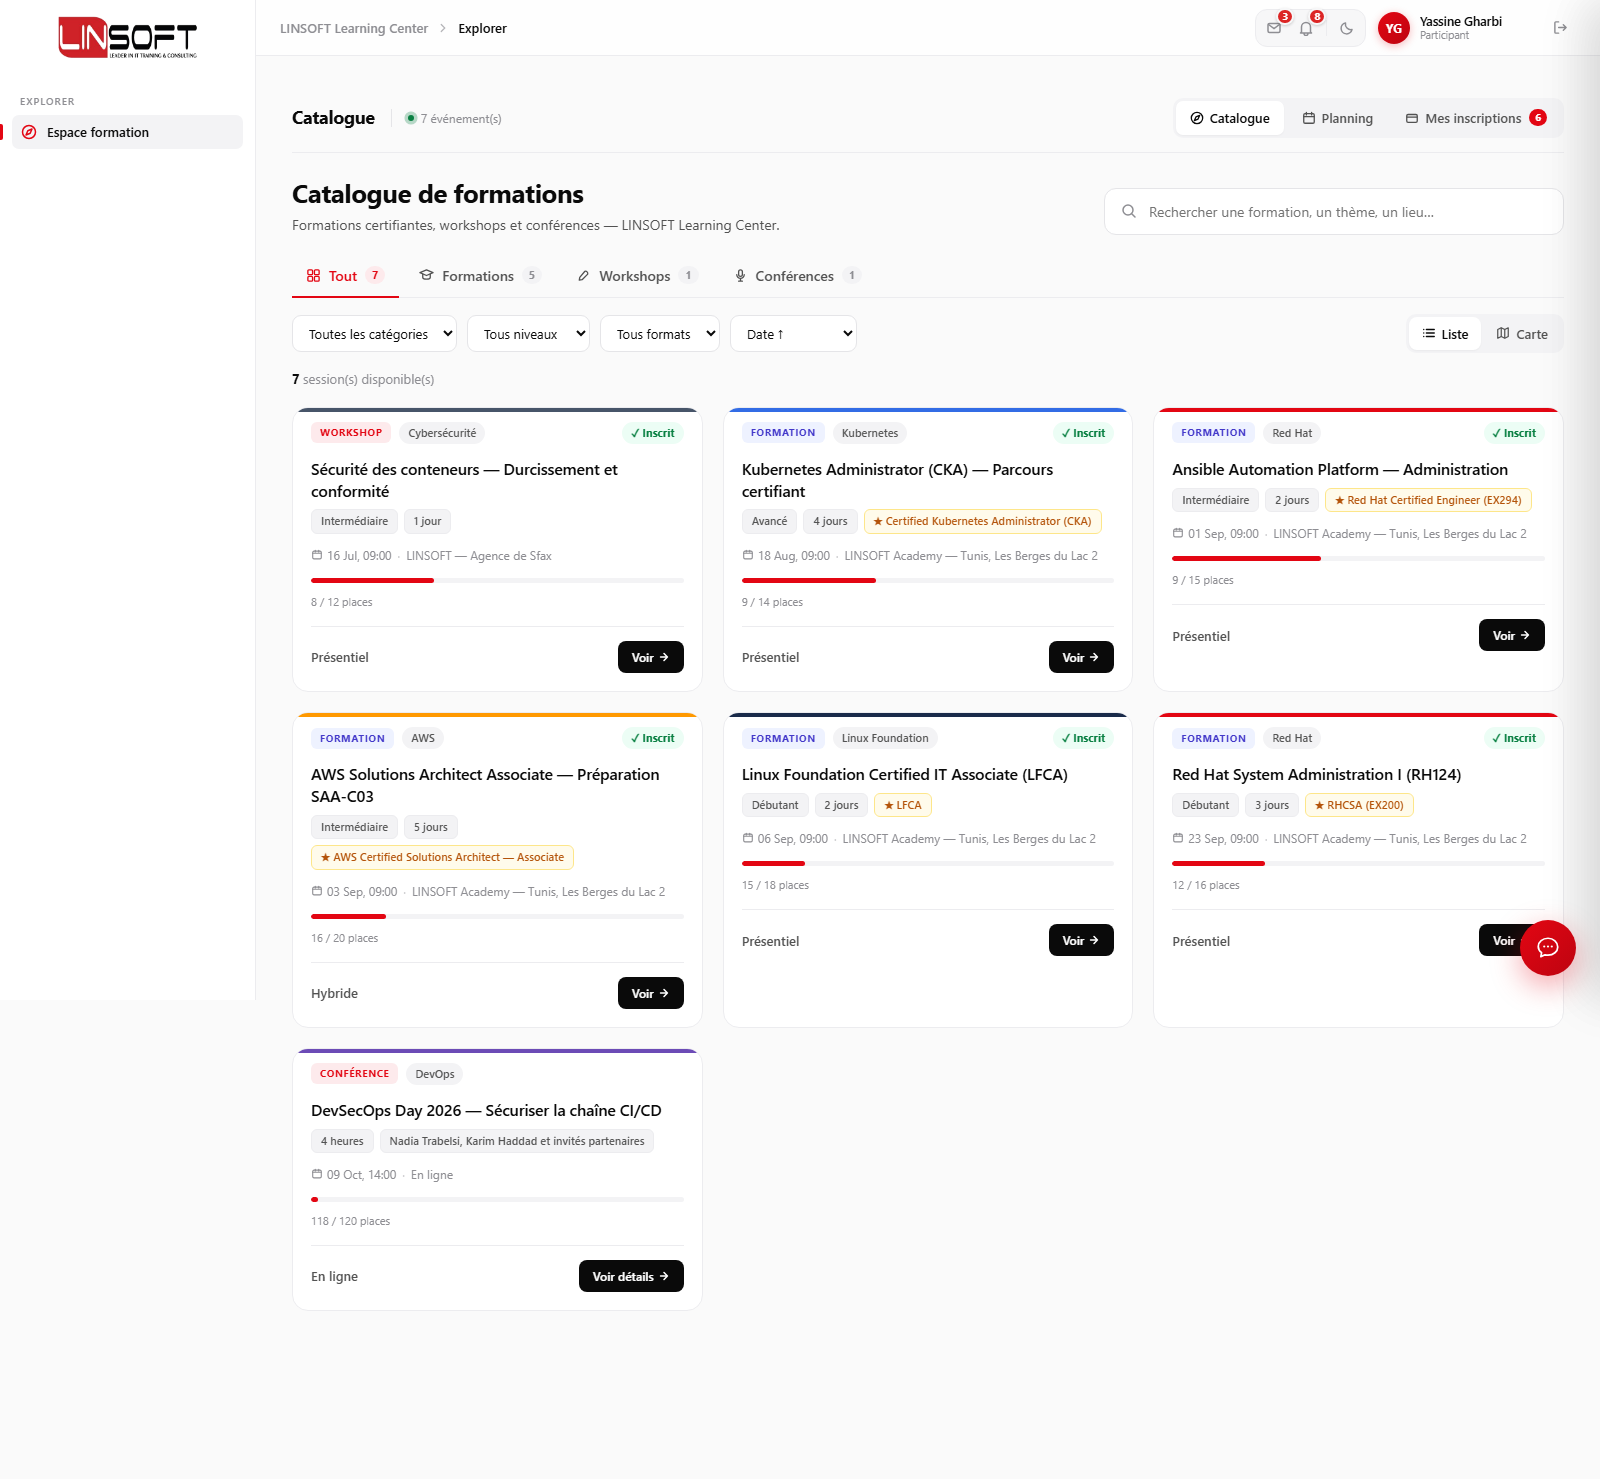
\includegraphics[width=0.92\textwidth]{captures/03-catalogue.png}
  \caption{Catalogue de formations — vue participant}
  \label{fig:devops-catalogue}
\end{figure}

%============================================================================
\section{Qualité du code et couverture}

\subsection{Outils d'analyse}
L'analyse statique (\textbf{Checkstyle} et \textbf{SpotBugs}) est regroupée dans un profil
Maven \texttt{quality}, activé à la demande et en intégration continue. Le jeu de règles
Checkstyle cible délibérément les défauts réels — comparaison de chaînes par
\texttt{==}, \texttt{equals} sans \texttt{hashCode}, blocs \texttt{catch} vides,
\texttt{switch} sans \texttt{default} — plutôt que la mise en forme : un jeu de règles trop
bavard finit systématiquement désactivé.

\subsection{Couverture mesurée}
\textbf{JaCoCo} produit des rapports HTML et XML par module. Le seuil est vérifié à chaque
\texttt{mvn verify} et fait échouer le build s'il n'est pas atteint.

\begin{table}[H]\centering\renewcommand{\arraystretch}{1.25}
\begin{tabular}{|p{5.5cm}|p{3cm}|}\hline
\rowcolor{gray!15}\textbf{Module} & \textbf{Couverture} \\ \hline
\texttt{feedback-service} & 78~\% \\ \hline
\texttt{notification-service} & 74~\% \\ \hline
\texttt{ticket-service} & 71~\% \\ \hline
\texttt{registration-service} & 61~\% \\ \hline
\texttt{event-service} & 53~\% \\ \hline
\texttt{ai-service} & 42~\% \\ \hline
\texttt{user-service} & 41~\% \\ \hline
\end{tabular}
\caption{Couverture des instructions, hors configuration, entités et DTO}\label{tab:couverture}
\end{table}

Le seuil a été relevé progressivement (0~\%, puis 25~\%, 30~\% et enfin 40~\%) au fur et à
mesure de l'écriture des tests. Ce choix est délibéré : un seuil ambitieux fixé d'emblée
aurait été inatteignable et n'aurait produit qu'une chose, sa propre désactivation. Le
seuil joue ainsi le rôle d'un \emph{cliquet anti-régression} plutôt que d'un objectif
décoratif. Son caractère réellement bloquant a été vérifié en le forçant temporairement à
90~\%, ce qui provoque bien l'échec du build.

%============================================================================
\section{Conteneurisation}

Chacun des onze composants dispose de son image. Les images backend reposent sur
\texttt{eclipse-temurin:17-jre-alpine} et appliquent \texttt{chgrp -R 0 /app}, condition
nécessaire sur OpenShift, qui exécute les conteneurs avec un identifiant utilisateur
aléatoire appartenant au groupe~0. Le frontend est construit en deux étapes
(\texttt{node:20-alpine} puis \texttt{nginx-unprivileged}) et s'exécute sans privilèges.

\subsection{Un défaut de conception corrigé}
Les images déclaraient déjà une directive \texttt{HEALTHCHECK} interrogeant
\texttt{/actuator/health}, \textbf{mais sept services sur dix n'embarquaient pas Actuator} :
la sonde recevait une réponse 404. Le fichier \texttt{docker-compose.yml} contournait le
problème par un \texttt{curl -s -o /dev/null || exit 1}, qui \emph{réussit même sur un 404
ou un 401}. Aucune vérification de santé du projet ne prouvait donc quoi que ce soit.
Actuator a été ajouté à tous les services via le POM parent, et les contournements
remplacés par de véritables vérifications.

%============================================================================
\section{Intégration et livraison continues}

\subsection{Architecture du pipeline}
La chaîne est décrite dans \texttt{.github/workflows/ci.yml} et s'exécute sur
\textbf{GitHub Actions} à chaque poussée et à chaque \emph{pull request}.

\begin{table}[H]\centering\renewcommand{\arraystretch}{1.25}
\begin{tabular}{|p{4cm}|p{9.5cm}|}\hline
\rowcolor{gray!15}\textbf{Étape} & \textbf{Contenu} \\ \hline
Tests backend & \texttt{mvn verify} : unitaires, API/sécurité, intégration, couverture \\ \hline
Analyse statique & Checkstyle et SpotBugs \\ \hline
Tests frontend & Vitest puis build de production \\ \hline
Images Docker & Onze images construites en parallèle \\ \hline
Analyse de sécurité & Trivy, vulnérabilités critiques et élevées \\ \hline
Publication & Registre GHCR, branche principale uniquement \\ \hline
Tests E2E & Plateforme complète démarrée, jeu de données semé, Playwright \\ \hline
\end{tabular}
\caption{Étapes de la chaîne d'intégration continue}\label{tab:pipeline}
\end{table}

\subsection{Choix : ne pas compiler dans les images}
Les fichiers \texttt{Dockerfile} du backend copient une archive JAR déjà construite plutôt
que de la compiler. Une construction multi-étapes par service recompilerait dix fois le même
réacteur Maven, pour un résultat identique. Le réacteur est donc construit \textbf{une
seule fois}, les archives circulent en artefact entre les étapes, et chaque image est
assemblée à partir du binaire validé : l'artefact testé et l'artefact publié sont ainsi le
même objet.

\subsection{Garde-fou contre les faux positifs}
Une étape vérifie explicitement qu'\textbf{aucun test d'intégration n'a été ignoré} alors
que Docker était disponible. Sans ce contrôle, un environnement dépourvu de Docker
produirait un pipeline vert trompeur, puisque les tests Testcontainers s'ignorent
automatiquement en l'absence de démon.

\subsection{Deux défauts révélés par les premières exécutions}
Aucun des deux n'était détectable en local, ce qui illustre précisément l'apport d'une
chaîne d'intégration continue.

\begin{enumerate}
  \item \textbf{Référence d'action non résolue.} Les onze tâches de construction d'images
        échouaient à l'étape « Set up job », c'est-à-dire \emph{avant} leur première
        instruction. Les étiquettes du dépôt \texttt{trivy-action} sont préfixées par
        \texttt{v} : la référence \texttt{@0.28.0} n'existait pas. GitHub Actions résout les
        actions avant de les exécuter, d'où un échec sans aucune trace dans les étapes.
  \item \textbf{Nom d'image refusé par le registre.} Une fois ce point corrigé, la
        construction, l'analyse Trivy et l'authentification réussissaient, mais la
        publication échouait — symptôme trompeur. Le compte GitHub s'écrit
        \texttt{Medamine009}, avec une majuscule, alors que GHCR n'accepte que des noms
        d'image en minuscules. Le nom est désormais normalisé avant usage.
\end{enumerate}

%============================================================================
\section{Supervision et observabilité}

\subsection{Points de mesure}
Tous les services exposent, via Actuator et Micrometer, un agrégat de santé, des sondes
distinctes de \emph{liveness} et de \emph{readiness}, ainsi que leurs métriques au format
Prometheus. L'exposition est volontairement restreinte aux points réellement utilisés :
\texttt{env}, \texttt{beans} et \texttt{heapdump} restent fermés.

\subsection{Collecte et visualisation}
Prometheus interroge les dix services toutes les quinze secondes ; Grafana en propose la
lecture. L'ensemble est placé derrière un profil Docker Compose afin de ne pas alourdir le
démarrage courant de la plateforme.

\begin{figure}[H]\centering
  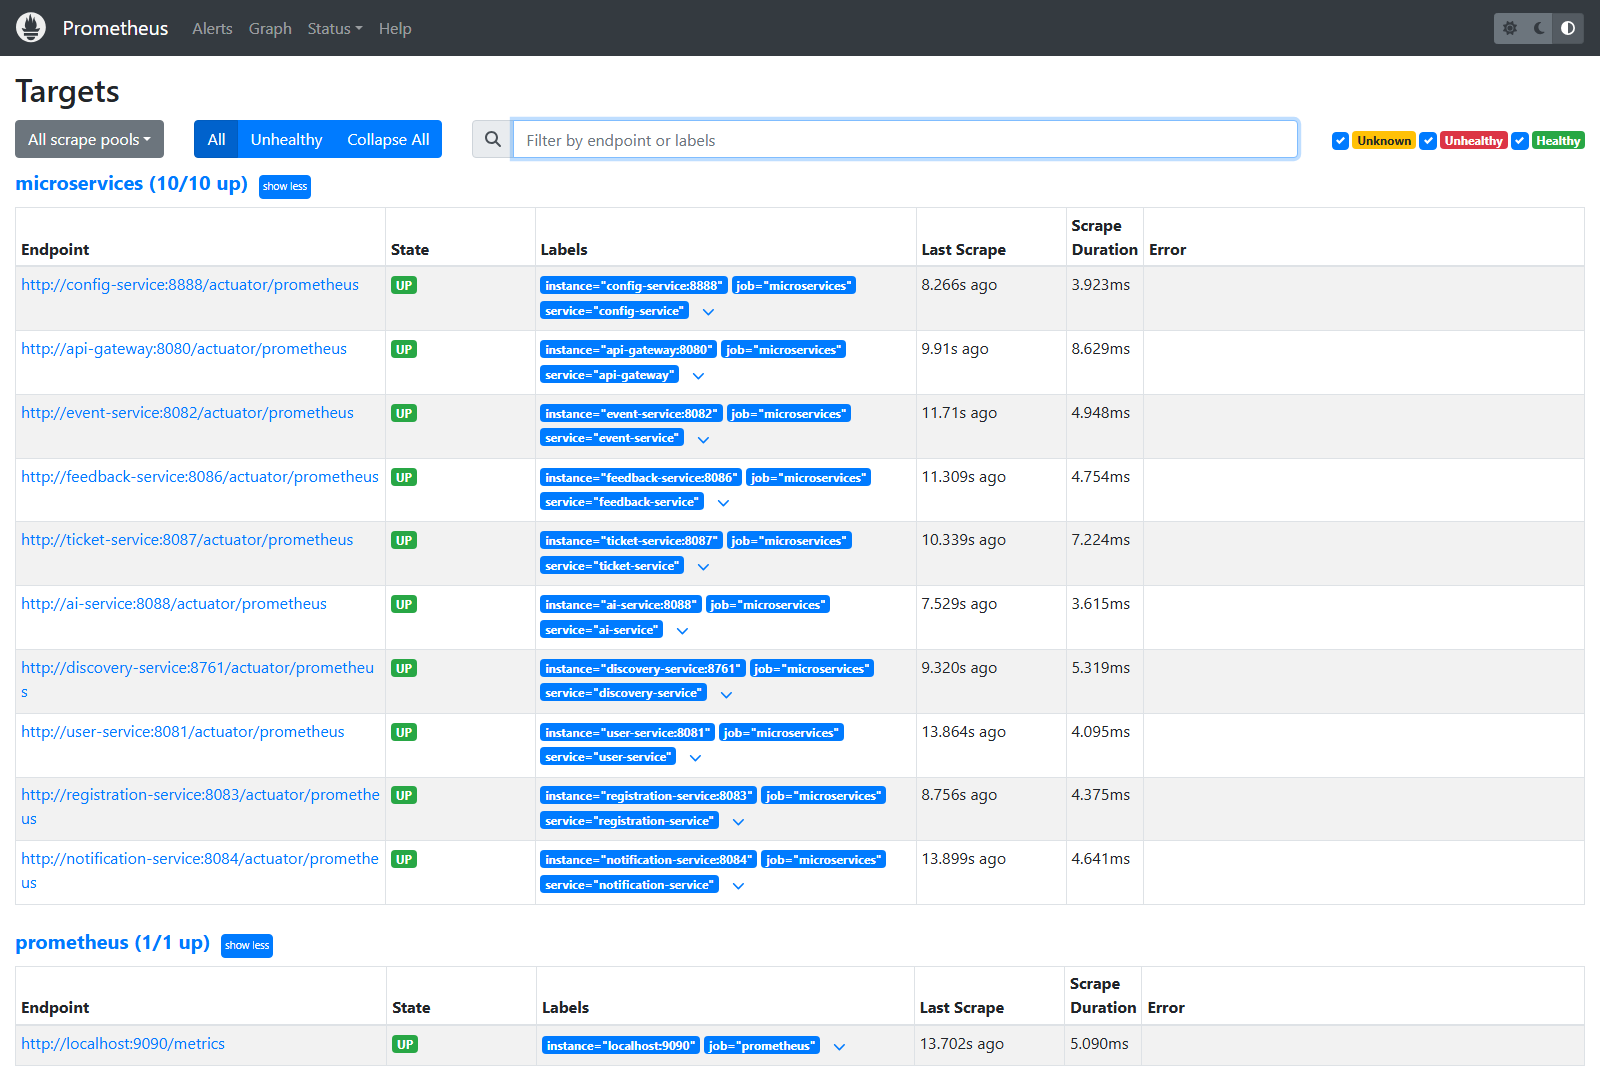
\includegraphics[width=0.92\textwidth]{captures/08-prometheus-cibles.png}
  \caption{Cibles Prometheus : les dix microservices interrogés avec succès}
  \label{fig:prometheus}
\end{figure}

\begin{figure}[H]\centering
  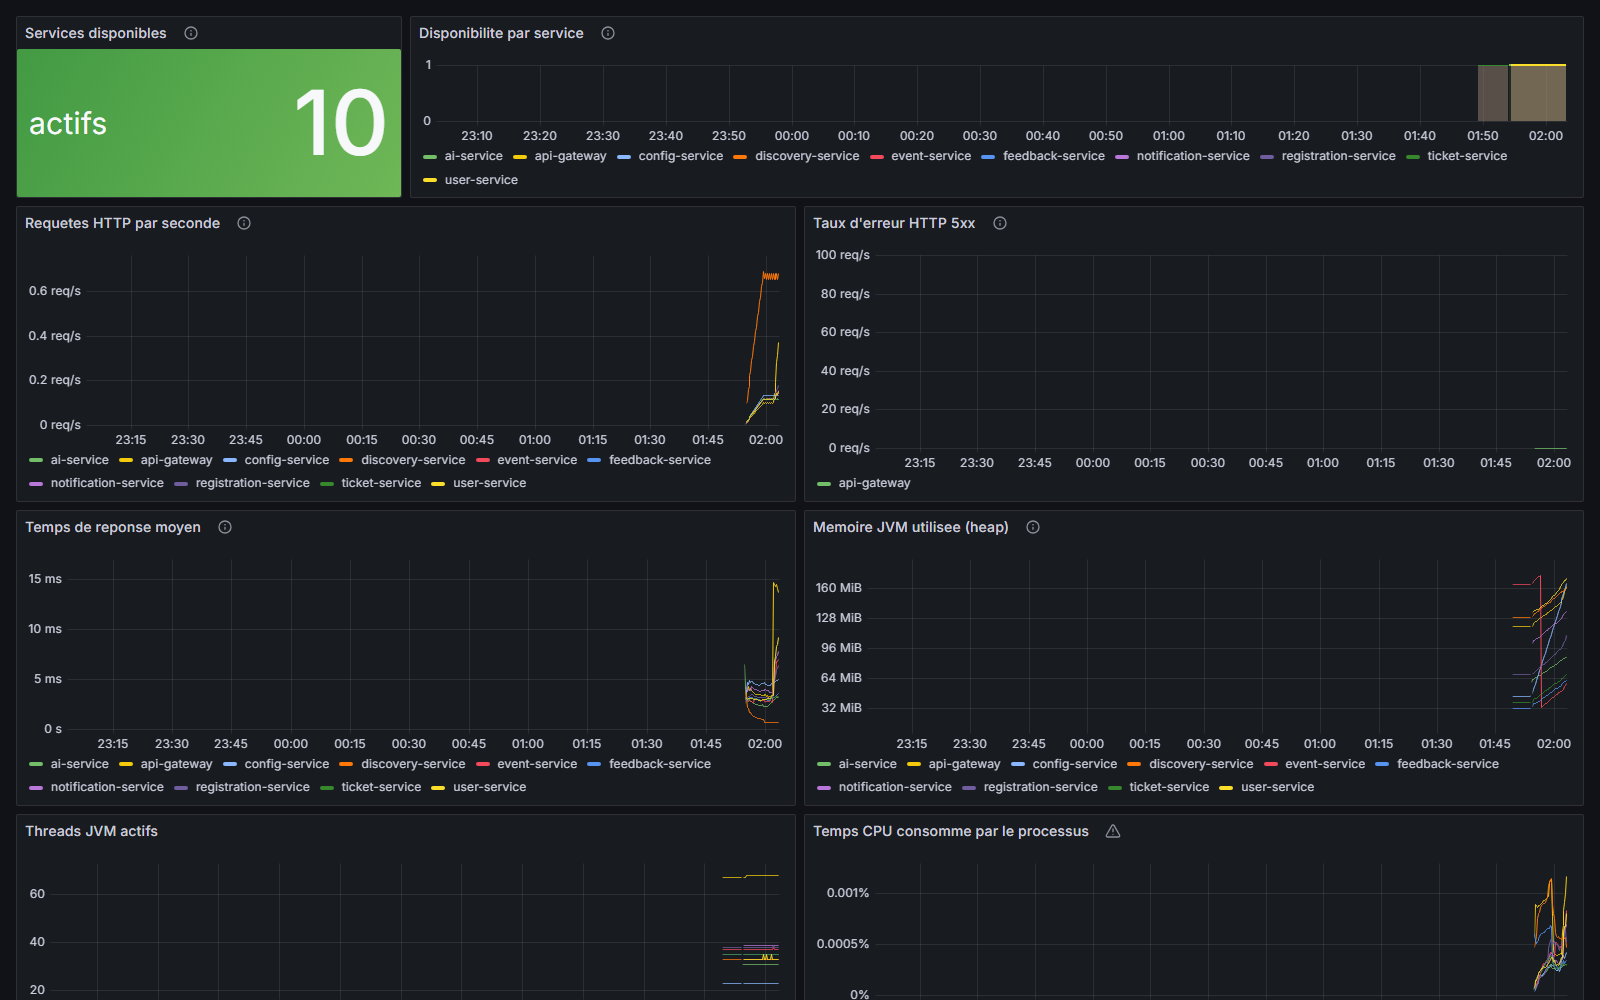
\includegraphics[width=\textwidth]{captures/09-grafana-plateforme.png}
  \caption{Tableau de bord Grafana : disponibilité, charge, temps de réponse et mémoire}
  \label{fig:grafana}
\end{figure}

Chaque série porte une étiquette \texttt{application} apposée par Micrometer ; sans elle,
les séries des dix services seraient indistinguables.

\begin{figure}[H]\centering
  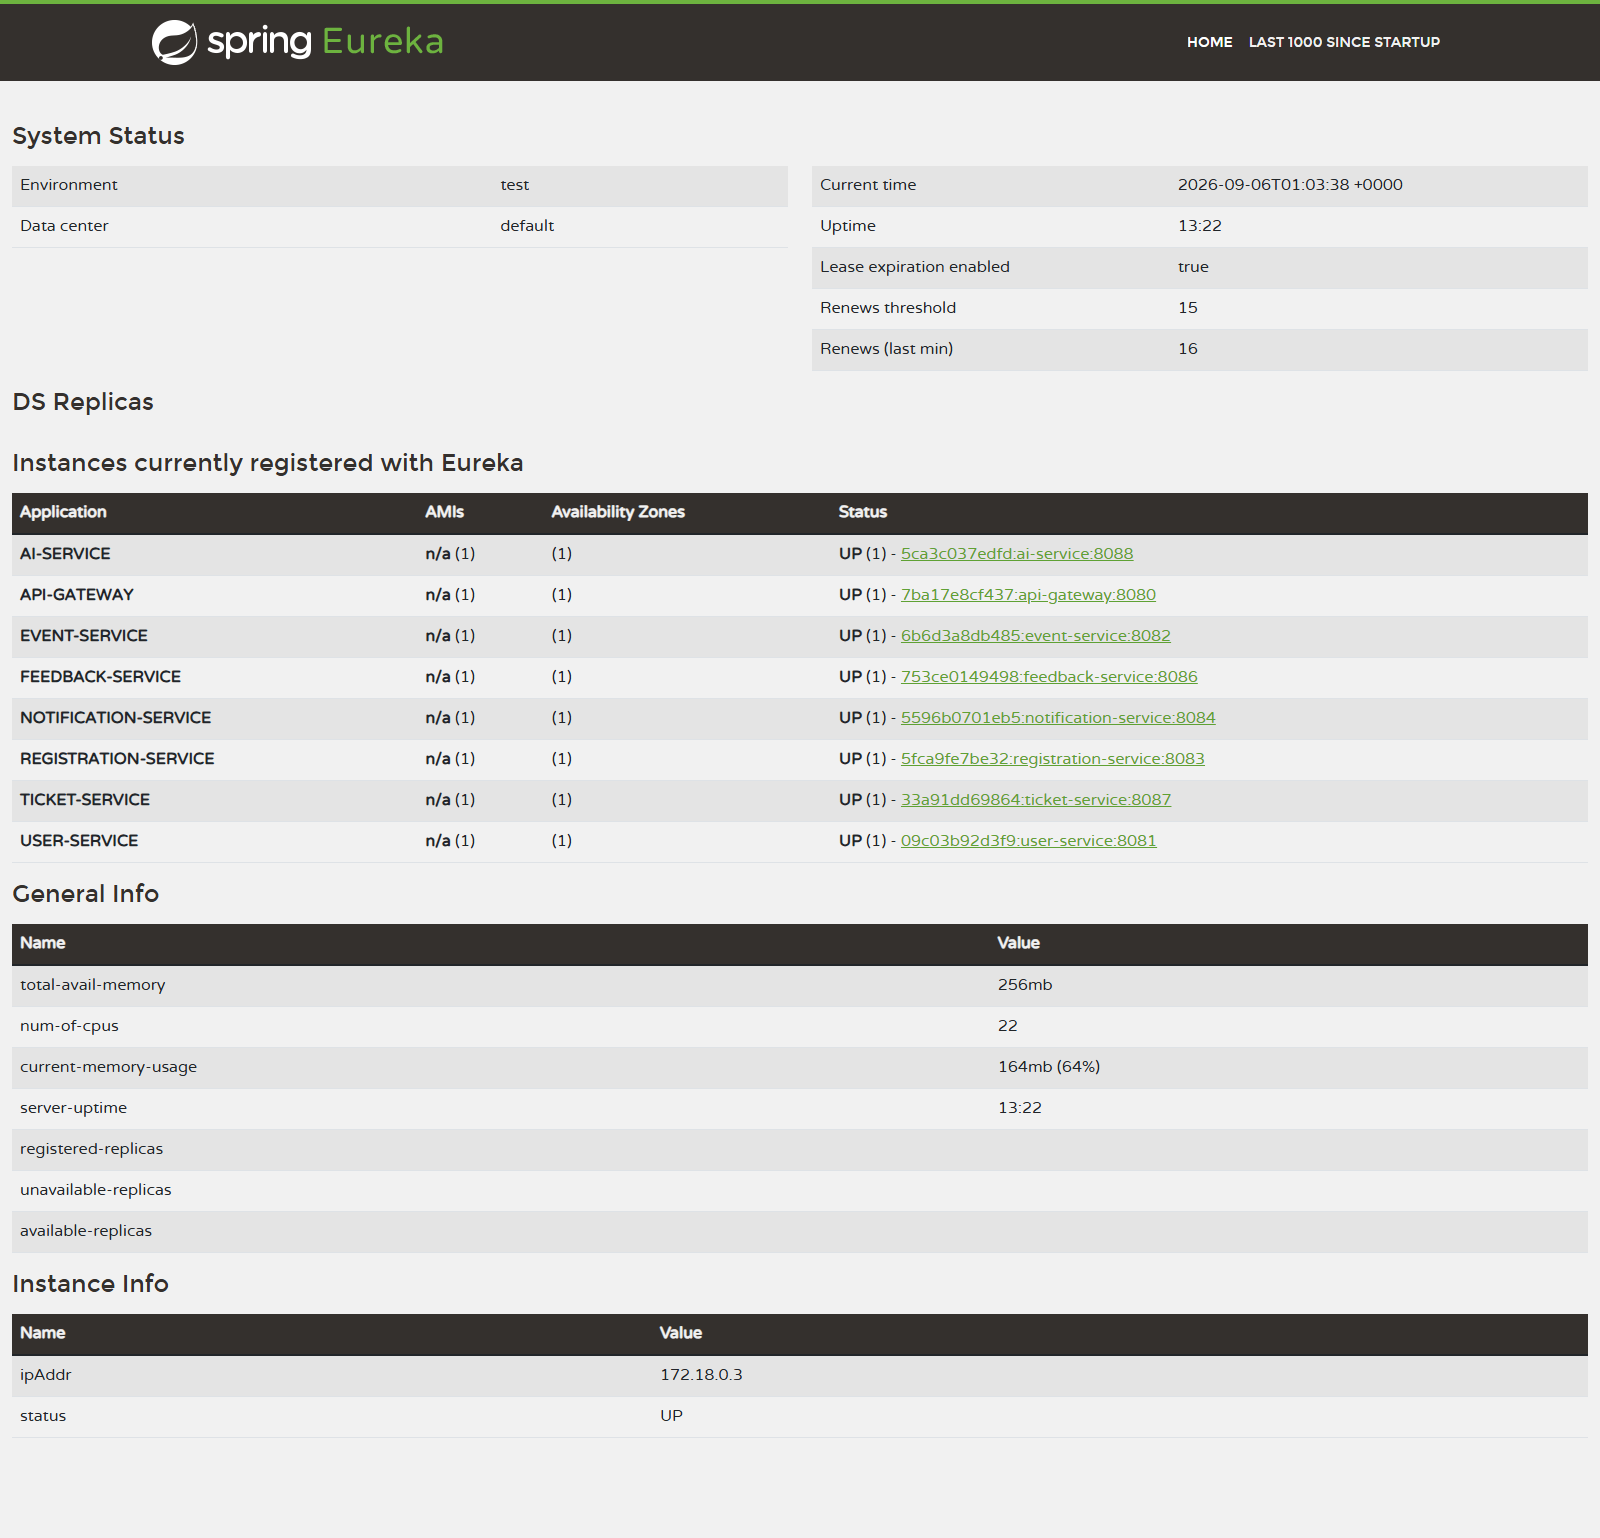
\includegraphics[width=0.92\textwidth]{captures/11-eureka.png}
  \caption{Registre Eureka : services enregistrés et découverte dynamique}
  \label{fig:eureka}
\end{figure}

\begin{figure}[H]\centering
  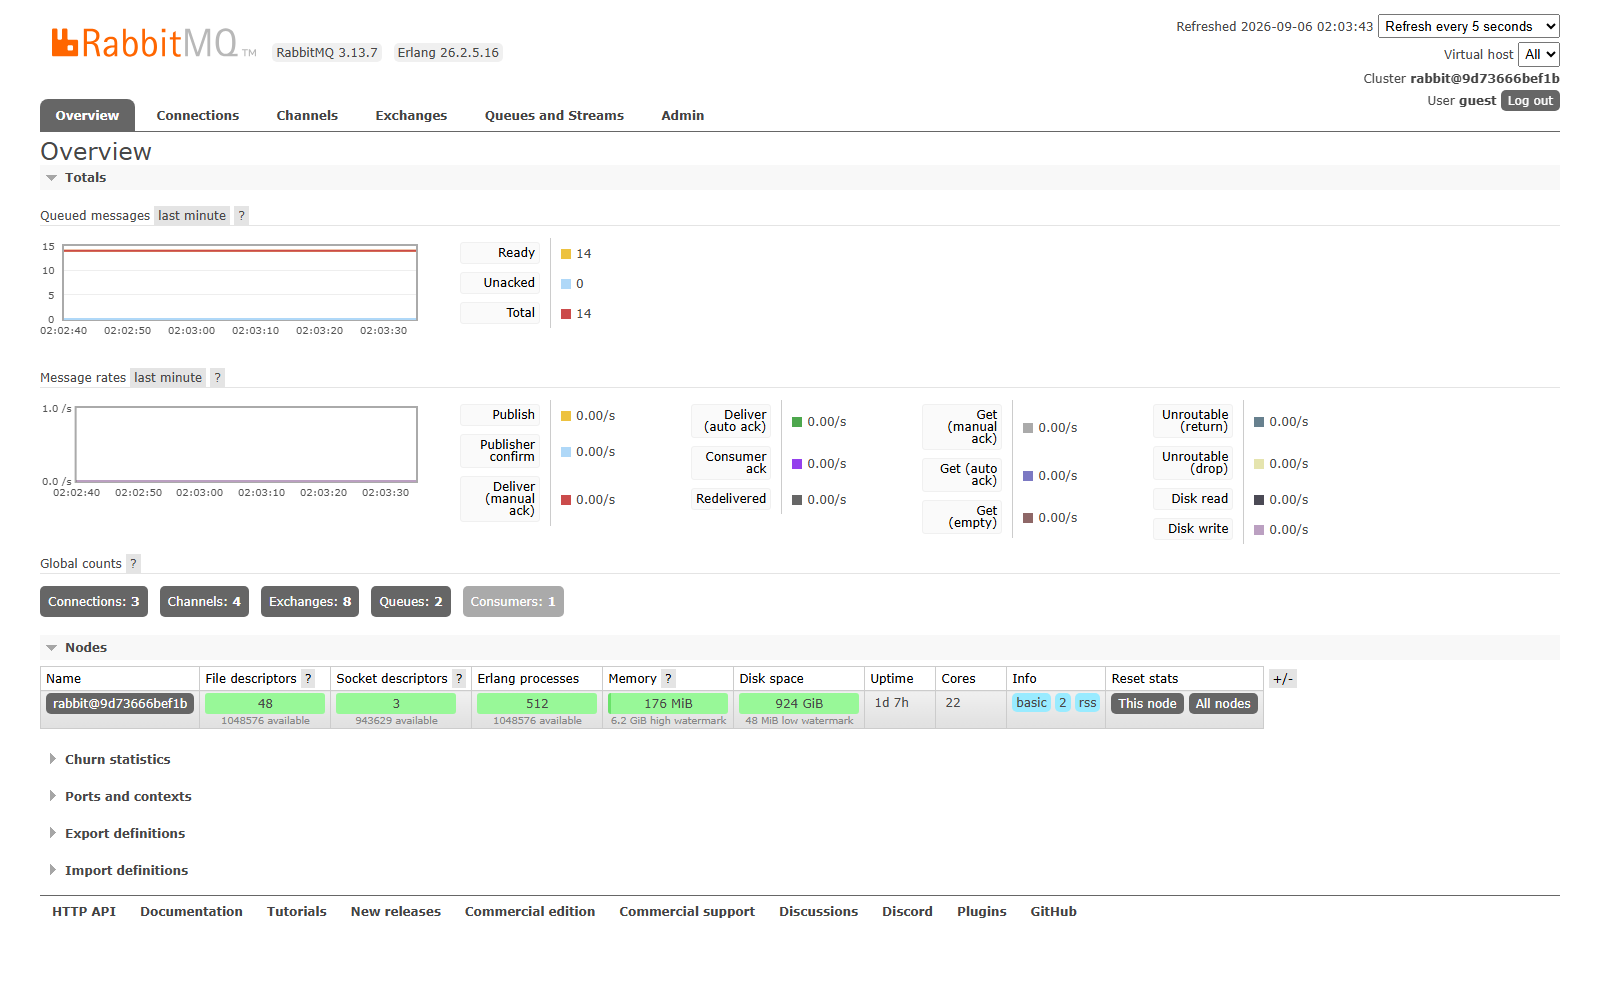
\includegraphics[width=0.92\textwidth]{captures/12-rabbitmq.png}
  \caption{Console RabbitMQ : file de notifications et débit des messages}
  \label{fig:rabbitmq}
\end{figure}

%============================================================================
\section{Sécurité de la chaîne}

\begin{itemize}
  \item \textbf{Analyse des images} : Trivy inspecte chaque image et remonte les
        vulnérabilités critiques et élevées dans l'onglet \emph{Security} du dépôt.
  \item \textbf{Aucun secret versionné} : la publication utilise le jeton fourni par la
        plateforme. Le fichier \texttt{.env} est exclu du dépôt et accompagné d'un modèle
        \texttt{.env.example}.
  \item \textbf{Secrets de déploiement} : un script \texttt{create-secrets.sh} génère des
        mots de passe aléatoires via \texttt{oc create secret}, de sorte qu'aucune valeur
        réelle ne transite par Git.
\end{itemize}

%============================================================================
\section{Illustrations du parcours fonctionnel}

Les captures suivantes montrent le résultat obtenu sur les fonctionnalités les plus
structurantes, avec le jeu de données de démonstration.

\begin{figure}[H]\centering
  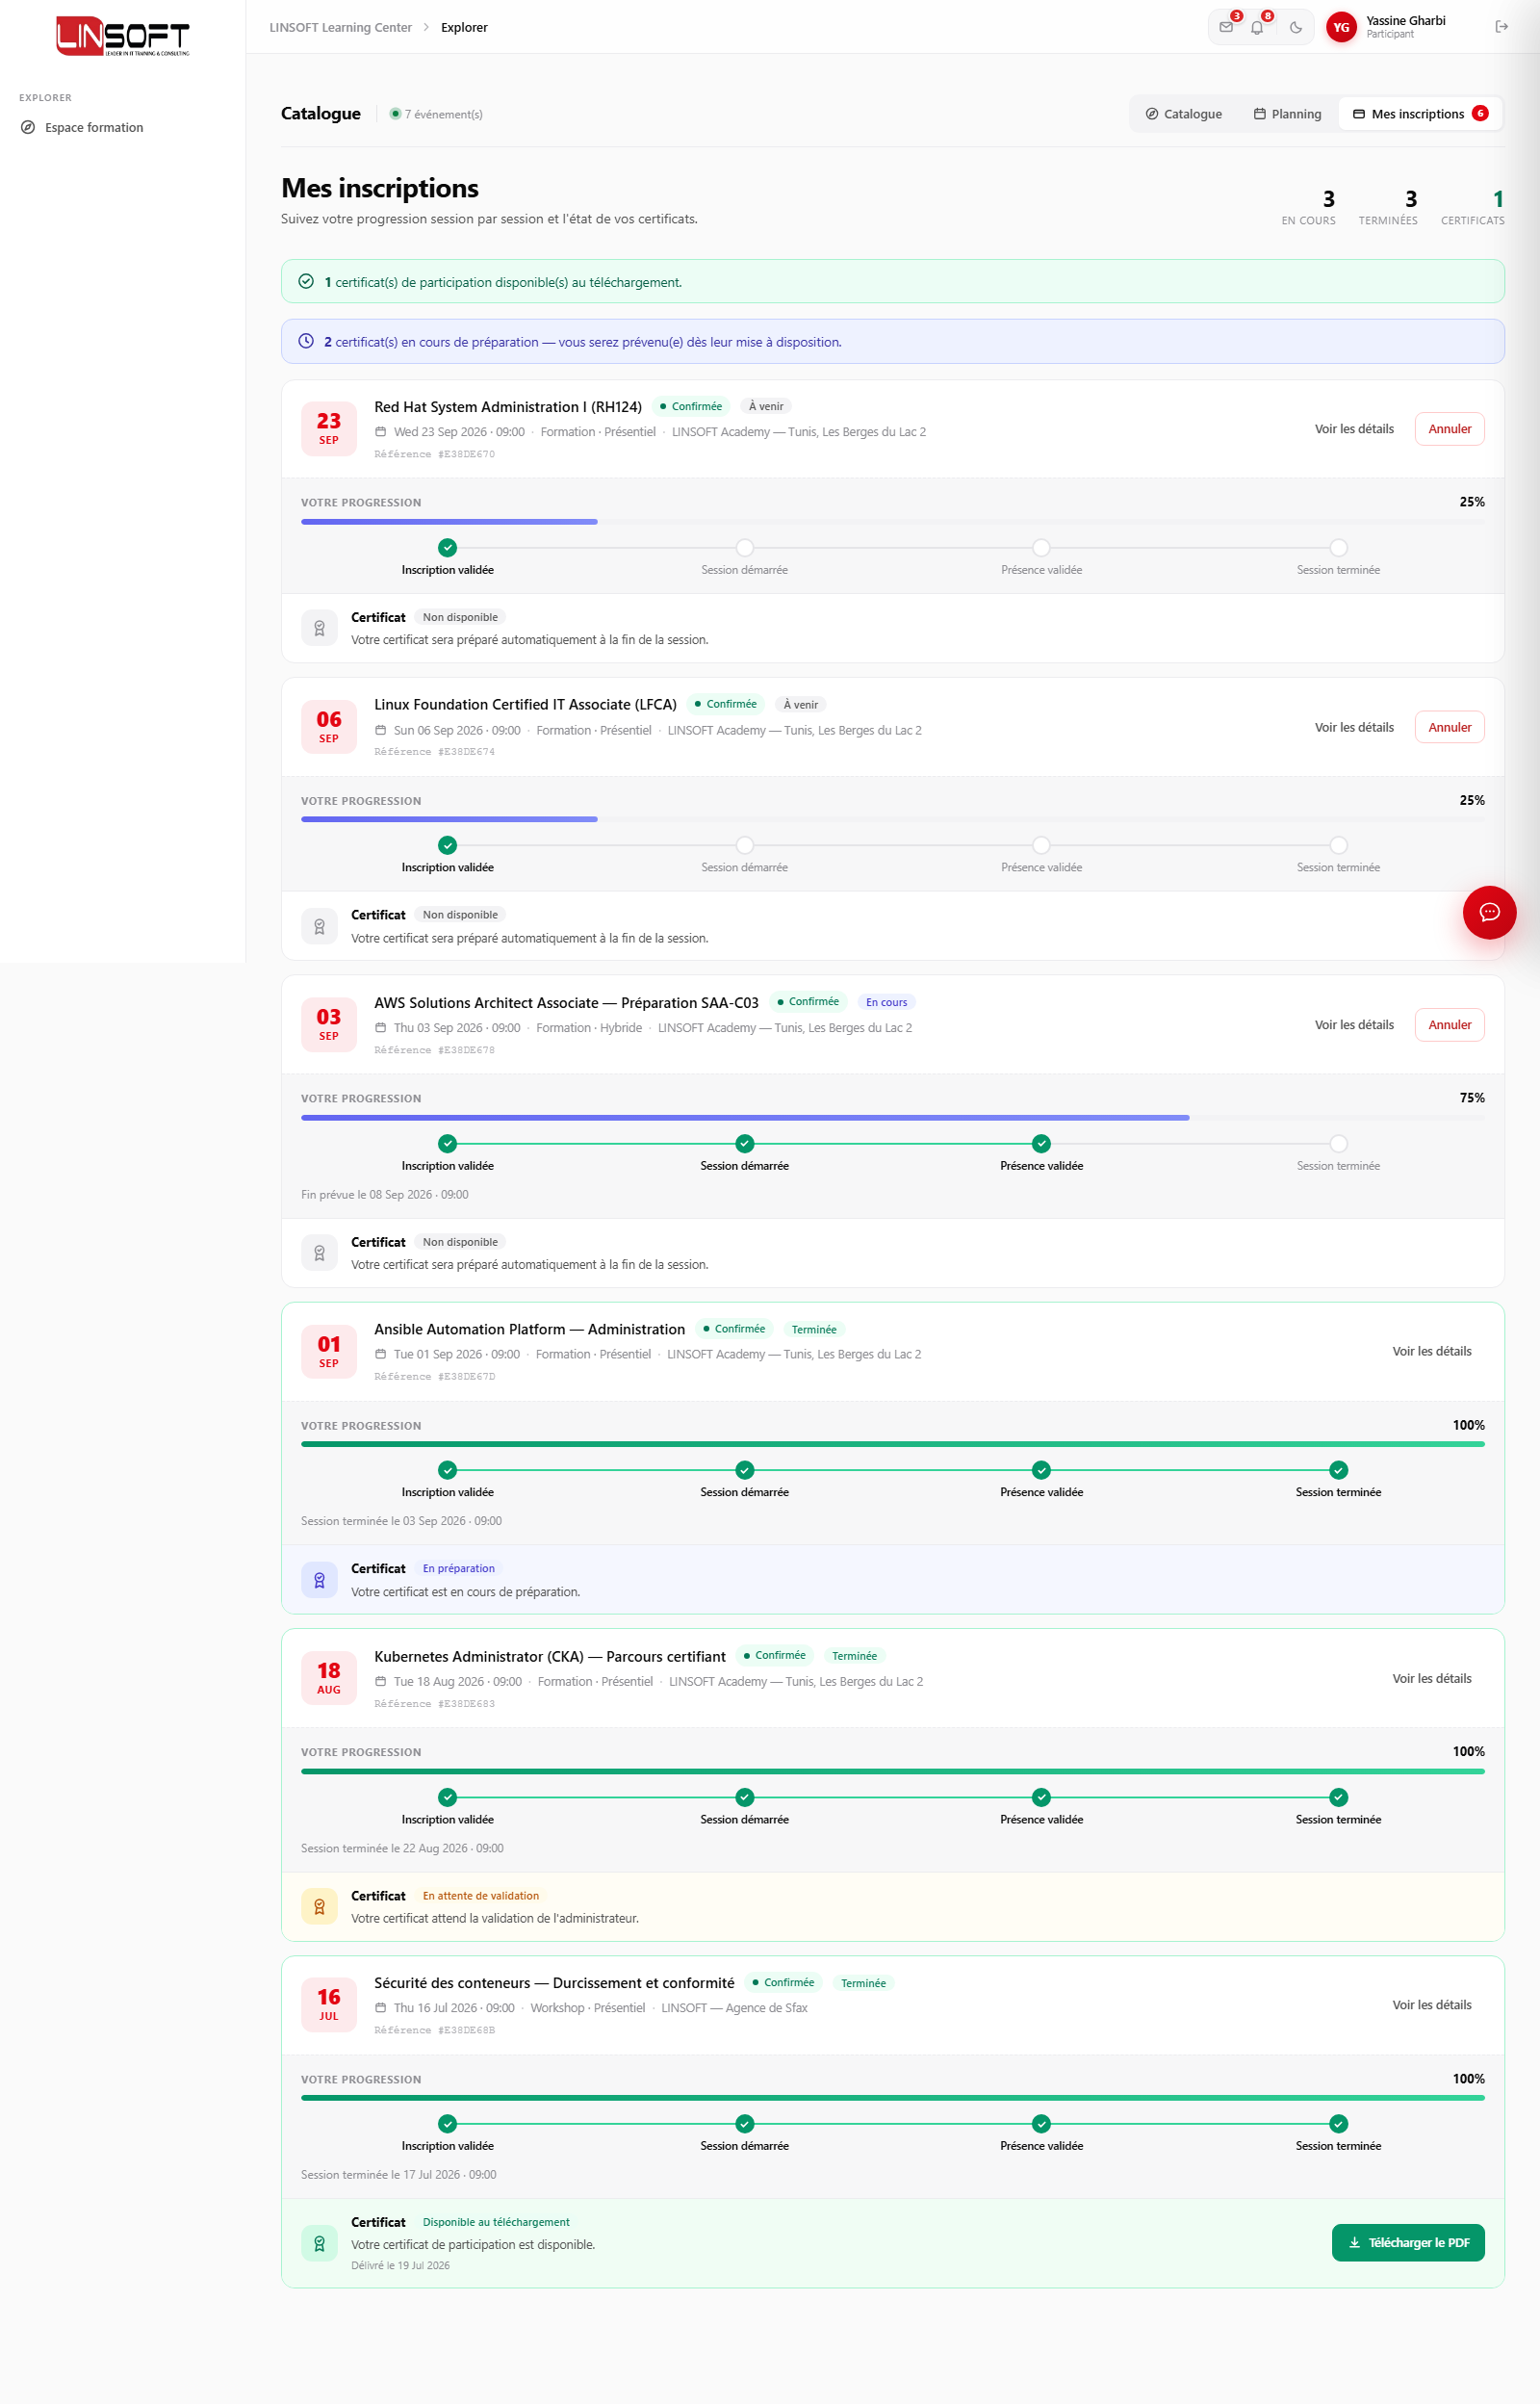
\includegraphics[width=0.85\textwidth]{captures/04-suivi-certificats.png}
  \caption{Suivi de participation : progression par jalons et cycle de vie du certificat}
  \label{fig:suivi}
\end{figure}

Cette vue rassemble les cinq états du parcours : session à venir (certificat non
disponible), session en cours avec progression intermédiaire, puis session terminée avec un
certificat successivement \emph{en préparation}, \emph{en attente de validation} et enfin
\emph{disponible au téléchargement}.

\begin{figure}[H]\centering
  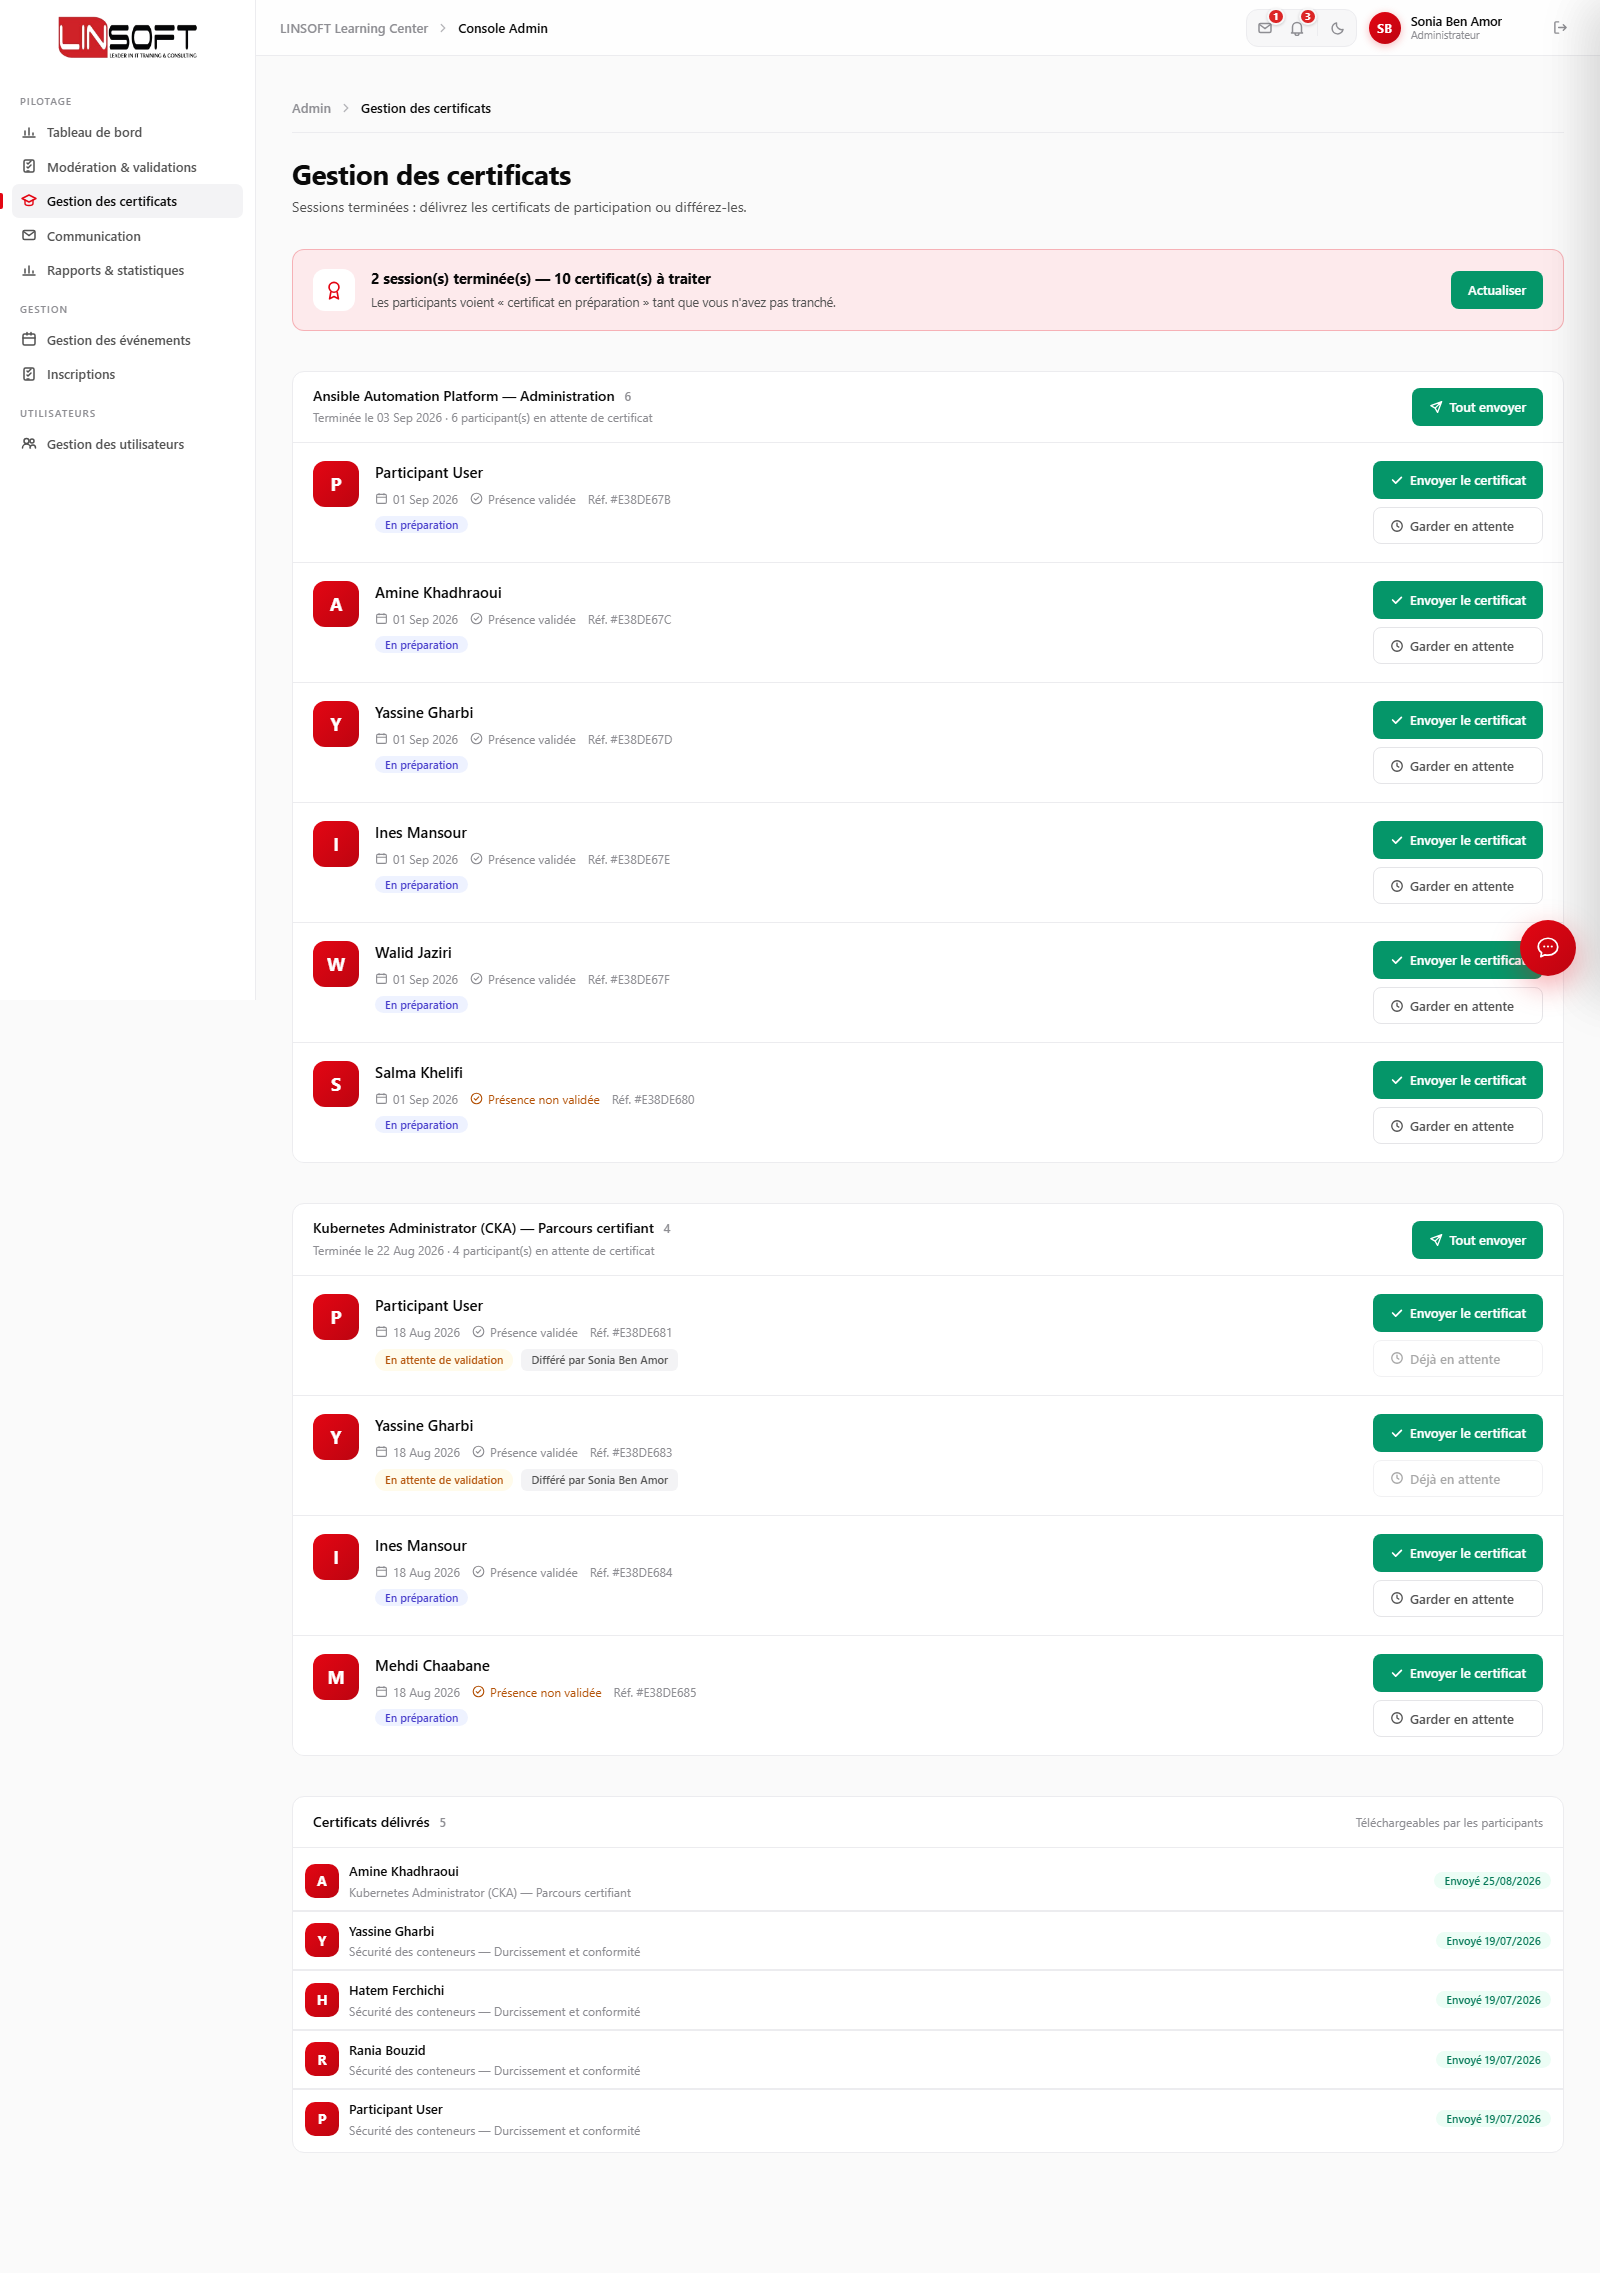
\includegraphics[width=0.85\textwidth]{captures/06-gestion-certificats.png}
  \caption{Console d'administration : file des certificats à délivrer, groupée par session}
  \label{fig:certificats-admin}
\end{figure}

\begin{figure}[H]\centering
  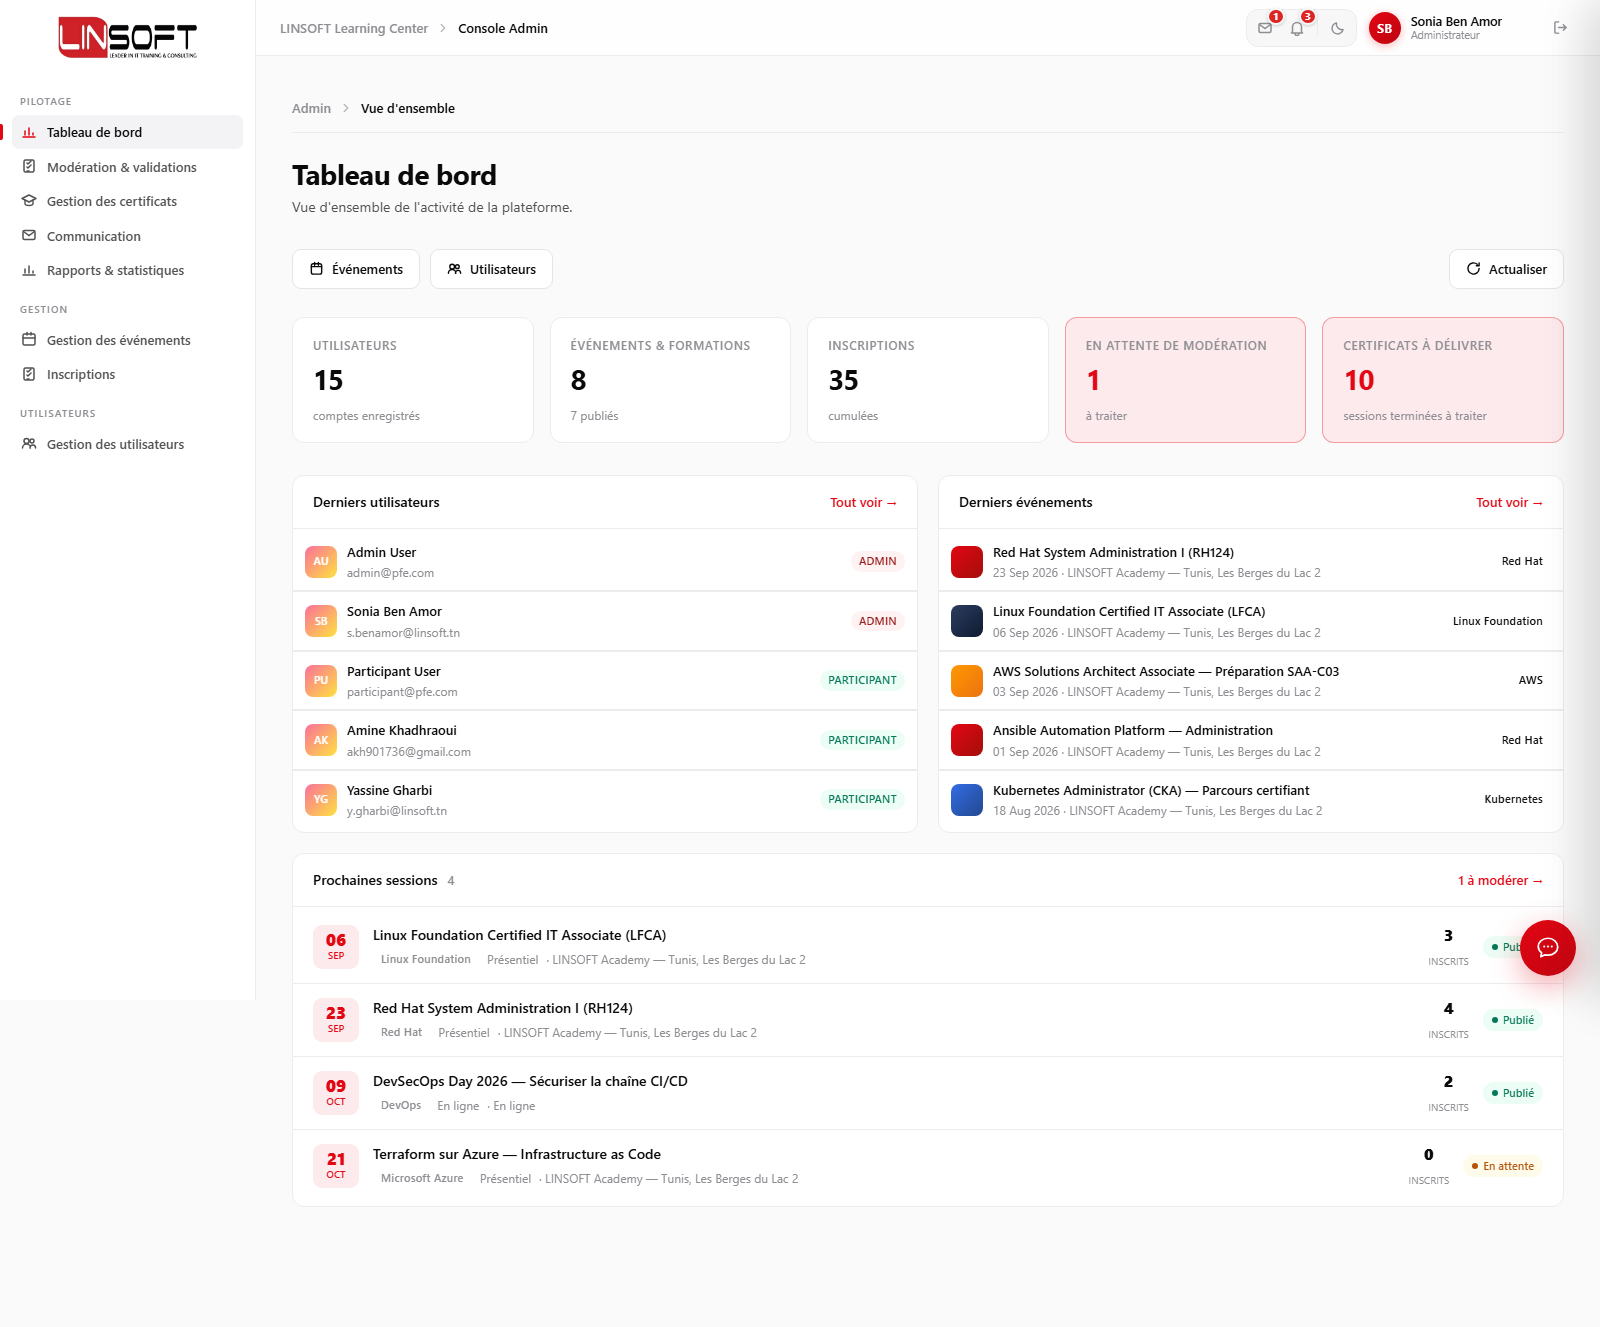
\includegraphics[width=0.92\textwidth]{captures/05-admin-dashboard.png}
  \caption{Tableau de bord administrateur et indicateurs de la plateforme}
  \label{fig:admin}
\end{figure}

\begin{figure}[H]\centering
  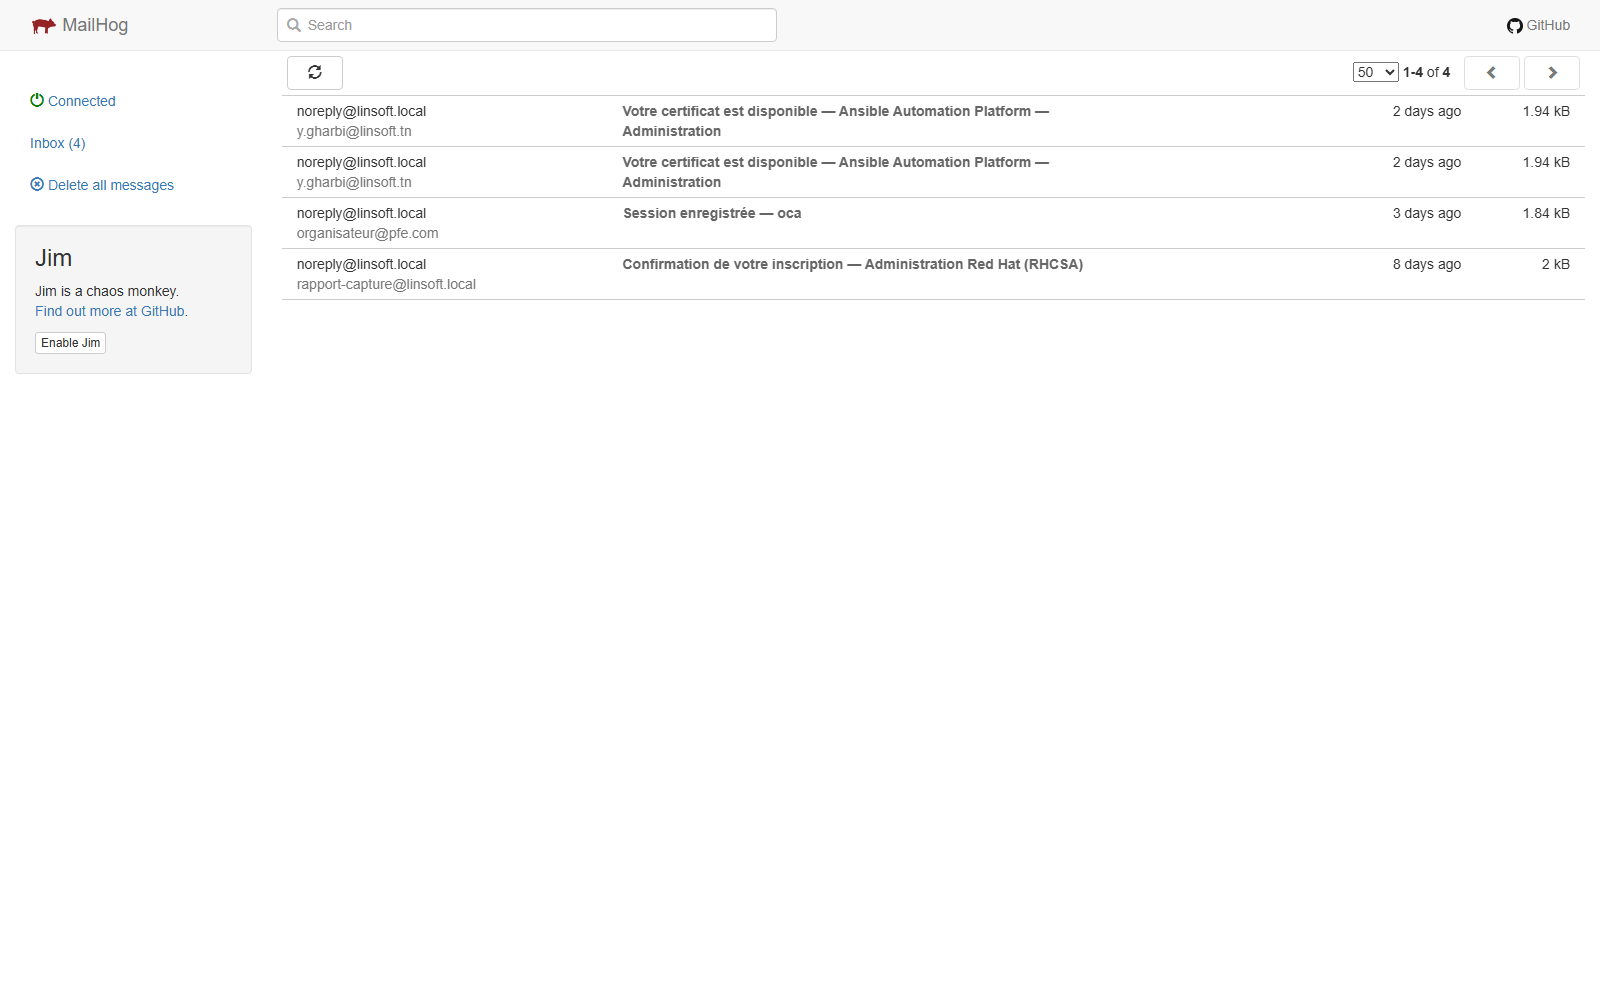
\includegraphics[width=0.92\textwidth]{captures/10-mailhog.png}
  \caption{Courriels émis par la plateforme, interceptés par MailHog en environnement de test}
  \label{fig:mailhog}
\end{figure}

%============================================================================
\section*{Conclusion}
La démarche présentée dans ce chapitre a fait passer le projet de dix-huit tests sans mesure
de couverture à près de trois cents tests répartis sur quatre niveaux, adossés à une chaîne
d'intégration continue de dix-sept tâches et à un dispositif de supervision opérationnel.
Au-delà des chiffres, cette démarche a démontré sa valeur en révélant des défauts réels et
invisibles autrement : des vérifications de santé qui ne vérifiaient rien, une référence
d'action inexistante, un nom d'image refusé par le registre, et une référence de dossier
identique pour toute une promotion de participants.
